%-------------------------------------------------------------------------------
% This file provides a skeleton ATLAS document.
%-------------------------------------------------------------------------------
% \pdfoutput=1
% The \pdfoutput command is needed by arXiv/JHEP/JINST to ensure use of pdflatex.
% It should be included in the first 5 lines of the file.
%-------------------------------------------------------------------------------
% Specify where ATLAS LaTeX style files can be found.
\newcommand*{\ATLASLATEXPATH}{latex/}
% Use this variant if the files are in a central location, e.g. $HOME/texmf.
% \newcommand*{\ATLASLATEXPATH}{}
%-------------------------------------------------------------------------------
\documentclass[UKenglish,texlive=2016]{\ATLASLATEXPATH atlasdoc}
% The language of the document must be set: usually UKenglish or USenglish.
% british and american also work!
% Commonly used options:
%  texlive=YYYY          Specify TeX Live version (2016 is default).
%  atlasstyle=true|false Use ATLAS style for document (default).
%  coverpage             Create ATLAS draft cover page for collaboration circulation.
%                        See atlas-draft-cover.tex for a list of variables that should be defined.
%  cernpreprint          Create front page for a CERN preprint.
%                        See atlas-preprint-cover.tex for a list of variables that should be defined.
%  PAPER                 The document is an ATLAS paper (draft).
%  CONF                  The document is a CONF note (draft).
%  PUB                   The document is a PUB note (draft).
%  BOOK                  The document is of book form, like an LOI or TDR (draft)
%  txfonts=true|false    Use txfonts rather than the default newtx - needed for arXiv submission.
%  paper=a4|letter       Set paper size to A4 (default) or letter.

%-------------------------------------------------------------------------------
% Extra packages:
\usepackage{\ATLASLATEXPATH atlaspackage}
% Commonly used options:
%  biblatex=true|false   Use biblatex (default) or bibtex for the bibliography.
%  backend=biber         Use the biber backend rather than bibtex.
%  subfigure|subfig|subcaption  to use one of these packages for figures in figures.
%  minimal               Minimal set of packages.
%  default               Standard set of packages.
%  full                  Full set of packages.
%-------------------------------------------------------------------------------
% Style file with biblatex options for ATLAS documents.
\usepackage{\ATLASLATEXPATH atlasbiblatex}

% Package for creating list of authors and contributors to the analysis.
\usepackage{\ATLASLATEXPATH atlascontribute}

% Useful macros
\usepackage{\ATLASLATEXPATH atlasphysics}
% See doc/atlas_physics.pdf for a list of the defined symbols.
% Default options are:
%   true:  journal, misc, particle, unit, xref
%   false: BSM, heppparticle, hepprocess, hion, jetetmiss, math, process, other, texmf
% See the package for details on the options.

% Files with references for use with biblatex.
% Note that biber gives an error if it finds empty bib files.
\addbibresource{qgnote.bib}
\addbibresource{bibtex/bib/ATLAS.bib}
\addbibresource{bibtex/bib/CMS.bib}
\addbibresource{bibtex/bib/ConfNotes.bib}
\addbibresource{bibtex/bib/PubNotes.bib}

% Paths for figures - do not forget the / at the end of the directory name.
\graphicspath{{logos/}{figures/}}

% Add you own definitions here (file qgnote-defs.sty).
\usepackage{qgnote-defs}

%-------------------------------------------------------------------------------
% Generic document information
%-------------------------------------------------------------------------------

% Title, abstract and document 
%-------------------------------------------------------------------------------
% This file contains the title, author and abstract.
% It also contains all relevant document numbers used by the different cover pages.
%-------------------------------------------------------------------------------

% Title
\AtlasTitle{Quark versus Gluon Jet Tagging Using Jet Images with the ATLAS Detector}

% Author - this does not work with revtex (add it after \begin{document})
%\author{The ATLAS Collaboration}

% Authors and list of contributors to the analysis
% \AtlasAuthorContributor also adds the name to the author list
% Include package latex/atlascontribute to use this
% Use authblk package if there are multiple authors, which is included by latex/atlascontribute
% \usepackage{authblk}
% Use the following 3 lines to have all institutes on one line
% \makeatletter
% \renewcommand\AB@affilsepx{, \protect\Affilfont}
% \makeatother
% \renewcommand\Authands{, } % avoid ``. and'' for last author
% \renewcommand\Affilfont{\itshape\small} % affiliation formatting
% \AtlasAuthorContributor{First AtlasAuthorContributor}{a}{Author's contribution.}
% \AtlasAuthorContributor{Second AtlasAuthorContributor}{b}{Author's contribution.}
%\AtlasAuthorContributor{Third AtlasAuthorContributor}{a}{Author's contribution.}
% \AtlasContributor{Fourth AtlasContributor}{Contribution to the analysis.}
 \AtlasAuthorContributor{Zihao Jiang}{a}{Main analyzer.}
 \AtlasAuthorContributor{Benjamin Nachman}{b}{Image plots, LLH studies, editing.}
 \AtlasAuthorContributor{Francesco Rubbo}{c}{Analyzer, editing.}
 \AtlasAuthorContributor{Ariel Schwartzman}{c}{advising}
\AtlasAuthorContributor{Lauren Tompkins}{a}{advising}
\affil[a]{Stanford University}
\affil[b]{LBNL}
 \affil[c]{SLAC}

% If a special author list should be indicated via a link use the following code:
% Include the two lines below if you do not use atlasstyle:
% \usepackage[marginal,hang]{footmisc}
% \setlength{\footnotemargin}{0.5em}
% Use the following lines in all cases:
% \usepackage{authblk}
% \author{The ATLAS Collaboration%
% \thanks{The full author list can be found at:\newline
%   \url{https://atlas.web.cern.ch/Atlas/PUBNOTES/ATL-PHYS-PUB-2016-007/authorlist.pdf}}
% }

% Draft version:
% Should be 1.0 for the first circulation, and 2.0 for the second circulation.
% If given, adds draft version on front page, a 'DRAFT' box on top of each other page, 
% and line numbers.
% Comment or remove in final version.
\AtlasVersion{1.0}

% ATLAS reference code, to help ATLAS members to locate the paper
\AtlasRefCode{PUB-JETM-2017-04}

% ATLAS note number. Can be an COM, INT, PUB or CONF note
% \AtlasNote{ATLAS-CONF-2016-XXX}
% \AtlasNote{ATL-PHYS-PUB-2016-XXX}
% \AtlasNote{ATL-COM-PHYS-2016-XXX}

% CERN preprint number
% \PreprintIdNumber{CERN-PH-2016-XX}

% ATLAS date - arXiv submission; usually filled in by the Physics Office
% \AtlasDate{\today}

% ATLAS heading - heading at top of title page. Set for TDR etc.
% \AtlasHeading{ATLAS ABC TDR}

% arXiv identifier
% \arXivId{14XX.YYYY}

% HepData record
% \HepDataRecord{ZZZZZZZZ}

% Submission journal and final reference
% \AtlasJournal{Phys.\ Lett.\ B.}
% \AtlasJournalRef{\PLB 789 (2014) 123}
% \AtlasDOI{}

% Abstract - % directly after { is important for correct indentation
\AtlasAbstract{%

Distinguishing quark-initiated from gluon-initiated jets is useful for many measurements and searches at the LHC.  
This note presents a jet \'tagger\' for distinguishing quark-initiated from gluon-initiated jets, which uses the full radiation 
pattern inside a jet processed as image in a deep neural network classifier.
The study is conducted using simulated dijet events in $\sqrt{s}=13$ TeV $pp$ collisions with the ATLAS detector.
Across a wide range of quark jet identification efficiencies, the neural network tagger achieves a gluon jet rejection that is comparable to or better than the performance 
of the jet width and track multiplicity observables conventionally used for quark-versus-gluon jet tagging.
}

%-------------------------------------------------------------------------------
% The following information is needed for the cover page. The commands are only defined
% if you use the coverpage option in atlasdoc or use the atlascover package
%-------------------------------------------------------------------------------

% List of supporting notes  (leave as null \AtlasCoverSupportingNote{} if you want to skip this option)
% \AtlasCoverSupportingNote{Short title note 1}{https://cds.cern.ch/record/XXXXXXX}
% \AtlasCoverSupportingNote{Short title note 2}{https://cds.cern.ch/record/YYYYYYY}
%
% OR (the 2nd option is deprecated, especially for CONF and PUB notes)
%
% Supporting material TWiki page  (leave as null \AtlasCoverTwikiURL{} if you want to skip this option)
% \AtlasCoverTwikiURL{https://twiki.cern.ch/twiki/bin/view/Atlas/WebHome}

% Comment deadline
% \AtlasCoverCommentsDeadline{10 July 2017}

% Analysis team members - contact editors should no longer be specified
% as there is a generic email list name for the editors
 %\AtlasCoverAnalysisTeam{Zihao Jiang, Benjamin Nachman, Francesco Rubbo, Ariel Schwartzman, Lauren Tompkins}

% Editorial Board Members - indicate the Chair by a (chair) after his/her name
% Give either all members at once (then they appear on one line), or separately
% \AtlasCoverEdBoardMember{EdBoard~Chair~(chair), EB~Member~1, EB~Member~2, EB~Member~3}
% \AtlasCoverEdBoardMember{EdBoard~Chair~(chair)}
% \AtlasCoverEdBoardMember{EB~Member~1}
% \AtlasCoverEdBoardMember{EB~Member~2}
% \AtlasCoverEdBoardMember{EB~Member~3}

% A PUB note has readers and not an EdBoard -- give their names here (one line or several entries)
% \AtlasCoverReaderMember{Reader~1, Reader~2}
% \AtlasCoverReaderMember{David Rousseau, Andy Buckley}

% Editors egroup
% \AtlasCoverEgroupEditors{atlas-GROUP-2016-XX-editors@cern.ch}

% EdBoard egroup
% \AtlasCoverEgroupEdBoard{atlas-GROUP-2016-XX-editorial-board@cern.ch}


% Author and title for the PDF file
\hypersetup{pdftitle={ATLAS document},pdfauthor={The ATLAS Collaboration}}

%-------------------------------------------------------------------------------
% Content
%-------------------------------------------------------------------------------
\begin{document}

\maketitle

\tableofcontents

% List of contributors - print here or after the Bibliography.
\PrintAtlasContribute{0.30}
\clearpage

%-------------------------------------------------------------------------------
\section{Introduction}
\label{sec:intro}
%-------------------------------------------------------------------------------

As discussed in Chapter \ref{chap:vbf}, the VBF \Hbb measurement requires identification of \bjets for both online and offline. Improvements of \btagging techniques can suppress the light and charm backgrounds and hence increase the sensitivity of \Hbb search. More importantly, improvement for online \btagging can lower the energy threshold for \bjet triggers and hence increase the efficiency of \Hbb event selections. This chapter focuses on improving the \btagging algorithm with Recurrent Neural Network (RNN). 

The most widely used and recommended \btagging algorithm within the ATLAS collaboration during the Run II LHC operation was \textit{MV2}. Briefly, the \textit{MV2} algorithm utilizes the different aspects of the $b$-hadron decay such as large impact parameters for its daughter tracks, existence of secondary vertex and so on. The algorithm is based on three low-level $b$-tagging algorithms: \textit{IP3D} (an impact parameter(IP)-based algorithms), \textit{SV1}(an inclusive secondary vertex-based algorithm), \textit{JetFitter} (a decay chain multi-vertex reconstruction algorithm)~\cite{ref:btagPaper}. The \textit{MV2} algorithm then takes the final and intermediate outputs from these baseline taggers as input and combines them through BDT~\cite{ATL-PHYS-PUB-2016-012}.

Many aspects of the \textit{MV2} algorithm can be improved despite its effectiveness. One could design better baseline algorithms or combination algorithm to improve \textit{MV2}. This thesis investigates particularly the improvement of the baseline algorithm \textit{IP3D}. This IP algorithm has the benefit that $b$-jet identification is possible even if no secondary vertex is explicitly reconstructed. The algorithm assigns per-track probabilities that a track is originated from a jet of a given flavor and take products of the marginal probabilities to estimate the likelihood. The per-track probabilities are estimated by referencing binned likelihood distributions from simulation while ignoring the potential correlations between them. This simplification is driven by a practical concern in the likelihood algorithm: accounting the correlations between tracks or the different track variables would need an estimation of the joint probabilities which have unmanageably large dimensions for binned linkelihood method.

To overcome these difficulties, the Recurrent Neural Network(RNN) is adopted. RNNs are a subclass of neural networks architectures that allow extensions to sequence-based and temporal domains (see~\cite{ref:RNNthesis} and references therein). They are typically used in natural language processing~\cite{languagemodel,DBLP:journals/corr/abs-1303-5778}, machine translation~\cite{MT,MT2}, and time-series analysis~\cite{timeseries,timeseries2}. In the case of $b$-tagging, the tracks in a $b$-jet can be treated as a variable-length sequence to recast $b$-tagging into a domain where RNNs have proven to be useful. This chapter presents the work of designing a new RNN-based \btagging algorithm called \textit{RNNIP}.


%%-------------------------------------------------------------------------------
%\section{ATLAS detector}
%\label{sec:detector}
%-------------------------------------------------------------------------------

%The ATLAS detector~\cite{PERF-2007-01} ...
% \input{atlas-detector}


%-------------------------------------------------------------------------------
\section{Quark and gluon jet images}
\label{sec:images}
%-------------------------------------------------------------------------------

\label{sec:cnn-image}
\subsection{Image Constituents}
For this study, jets clustered the anti-$k_t$ jet algorithm~\cite{Cacciari:2008gp}
are used and are required to have $|\eta|<2.1$ such that they remain fully within the
tracker coverage.
For reconstruction study, three types of constituents for jet image formations
are considered: tracks, calorimeter clusters and calorimeter towers. The truth level images
based on truth particles are also considered as performance benchmark as they have
higher qualities than images based on reconstructed quatities which are degraded by
finite detector resolution and noise. 

\subsubsection{tracks}
Track reconstructions follow the same procedure as described in Chapter\ref{chap:reconstruction}. Tight quality
criteria~\cite{ATL-PHYS-PUB-2015-051} on the track properties are used to mitigate the impact of pile-up as well as
to reject spurious (fake) tracks that result from multiple charged particles or noise.
Tracks used for this study are required to have $p_\text{T} > 0.5~\GeV$ and to originate from the hard-scatter primary vertex. 
Tracks are assigned to primary vertices based on the track-to-vertex matching resulting from the vertex reconstruction.
Tracks not included in vertex reconstruction are assigned to the nearest vertex based on the
distance $|\Delta z \times \sin\theta|$, up to a maximum distance of 3 mm.
The track to jet association scheme is ghost-association same as documented in Sec.\ref{sec:vbf-objsel}.


\subsubsection{calorimeter clusters}
The first type of energy information considered is topological calorimeter-cell 
clusters (topo-clusters)~\cite{PERF-2014-07}.
The algorithm uses as seeds calorimeter cells
with energy significance $|E_\text{cell}|/\sigma_\text{noise}>4$,
iteratively combines all neighbouring cells with
$|E_\text{cell}|/\sigma_\text{noise}>2$ and finally adds neighbouring cells
without any significance requirement.
%Topo-clusters at the EM scale are used as input for jet reconstruction with 
%with distance parameter $R=0.4$, as provided by FastJet~\cite{Cacciari:2011ma}.  

\subsubsection{calorimeter towers}
An alternative energy organization scheme, calorimeter towers,
is used to associate calorimeter information with the jets
reconstructed from topo-clusters.
Calorimeter towers are fixed-size objects ($\Delta\eta\times\Delta\phi=0.1\times0.1$)~\cite{cscbook}
that ensure a uniform segmentation of the calorimeter information.
Instead of building clusters, the cells are projected onto a fixed grid in $\eta$ and $\phi$ corresponding to 6400 towers
for the full calorimeter coverage $|\eta|<5$.
Calorimeter cells which completely fit within a tower contribute their total energy
to the single tower.
Cells which extend beyond the tower boundary contribute to multiple
towers, depending on the overlap fraction of the cell area with the towers.
In the following, towers are matched geometrically to jets built from topo-clusters, by considering all the towers within
the jet radius $R=0.4$.

%An overall jet calibration corrects the detector-level jet $p_\text{T}$ to the particle-level jet $p_\text{T}$ on average~\cite{Aad:2014bia}.   
\subsubsection{truth particles}
Truth-particle jets in Monte Carlo (MC) simulation are built from generated stable particles with a mean lifetime $\tau>30$~ps, 
excluding muons and neutrinos.
As with the detector-level jets, truth-particle jets are clustered with the anti-$k_t$ $R=0.4$ algorithm.
The $p_\text{T}$ of the truth-particle jet is used to select the jets.
Two $p_\text{T}$ ranges are considered for this study: $150~\GeV<p_\text{T}<200~\GeV$ and $400~\GeV<p_\text{T}<500~\GeV$.


\subsection{Image Formation}

There is an extensive literature on formation of jet images images. In line with the work such as~\cite{Cogan:2014oua,Almeida:2015jua}, the first step in constructing a jet image rotates and Lorentz boost all of the constituents inside a jet so that $\phi_\text{jet}=\eta_\text{jet}=0$. Then, the jet is cropped into a grid of size $16\times 16$ in $\eta$ and $\phi$ with pixel sizes $0.05\times 0.05$ and centered.  The intensity of each pixel is the total $p_\text{T}$ within the pixel, using a particular type of constituents (calorimeter-cell clusters, towers, tracks, or truth particles). Each image is then normalized so that $\sum_i I_i=1$, where $I_i$ is the intensity of the $i^\text{th}$ pixel. Normalization is performed for the tagger to learn only the information orthogonal to the jet transverse momentum.  %Normalization is known to remove useful discrimination information, but studies suggest the impact is small and it is useful for training. For an extensive description of the impact of image preprocessing on the information content of a jet image, see Ref.~\cite{deOliveira:2015xxd}.

One representative set of gluon jet images using different inputs is shown in Figure~\ref{fig:cnn-oneimage} and the average quark and gluon jet images and their differences are shown in Figure~\ref{fig:cnn-avg:truthtrack} and Figure~\ref{fig:cnn-avg:clustertower}. As clearly show, Jet images are extremely sparse. Only when shown in average form would one see a difference between quark and gluon jets in ensemble level. As expected, the radiation pattern around the core is broader for gluon jets relative to quark jets.
The slightly reduced central activity in track images shown in Figure~\ref{fig:cnn-avg:truthtrack} is compatible with the lower track reconstruction efficiency at the core of the jet~\cite{Aaboud:2017all}.
Topo-cluster images are found to be more collimated than tower images (Figure~\ref{fig:cnn-avg:clustertower}) as a result of the built-in noise suppression mechanism that removes some of the soft large-angle radiation.

\begin{figure}[htpb]
\begin{center}
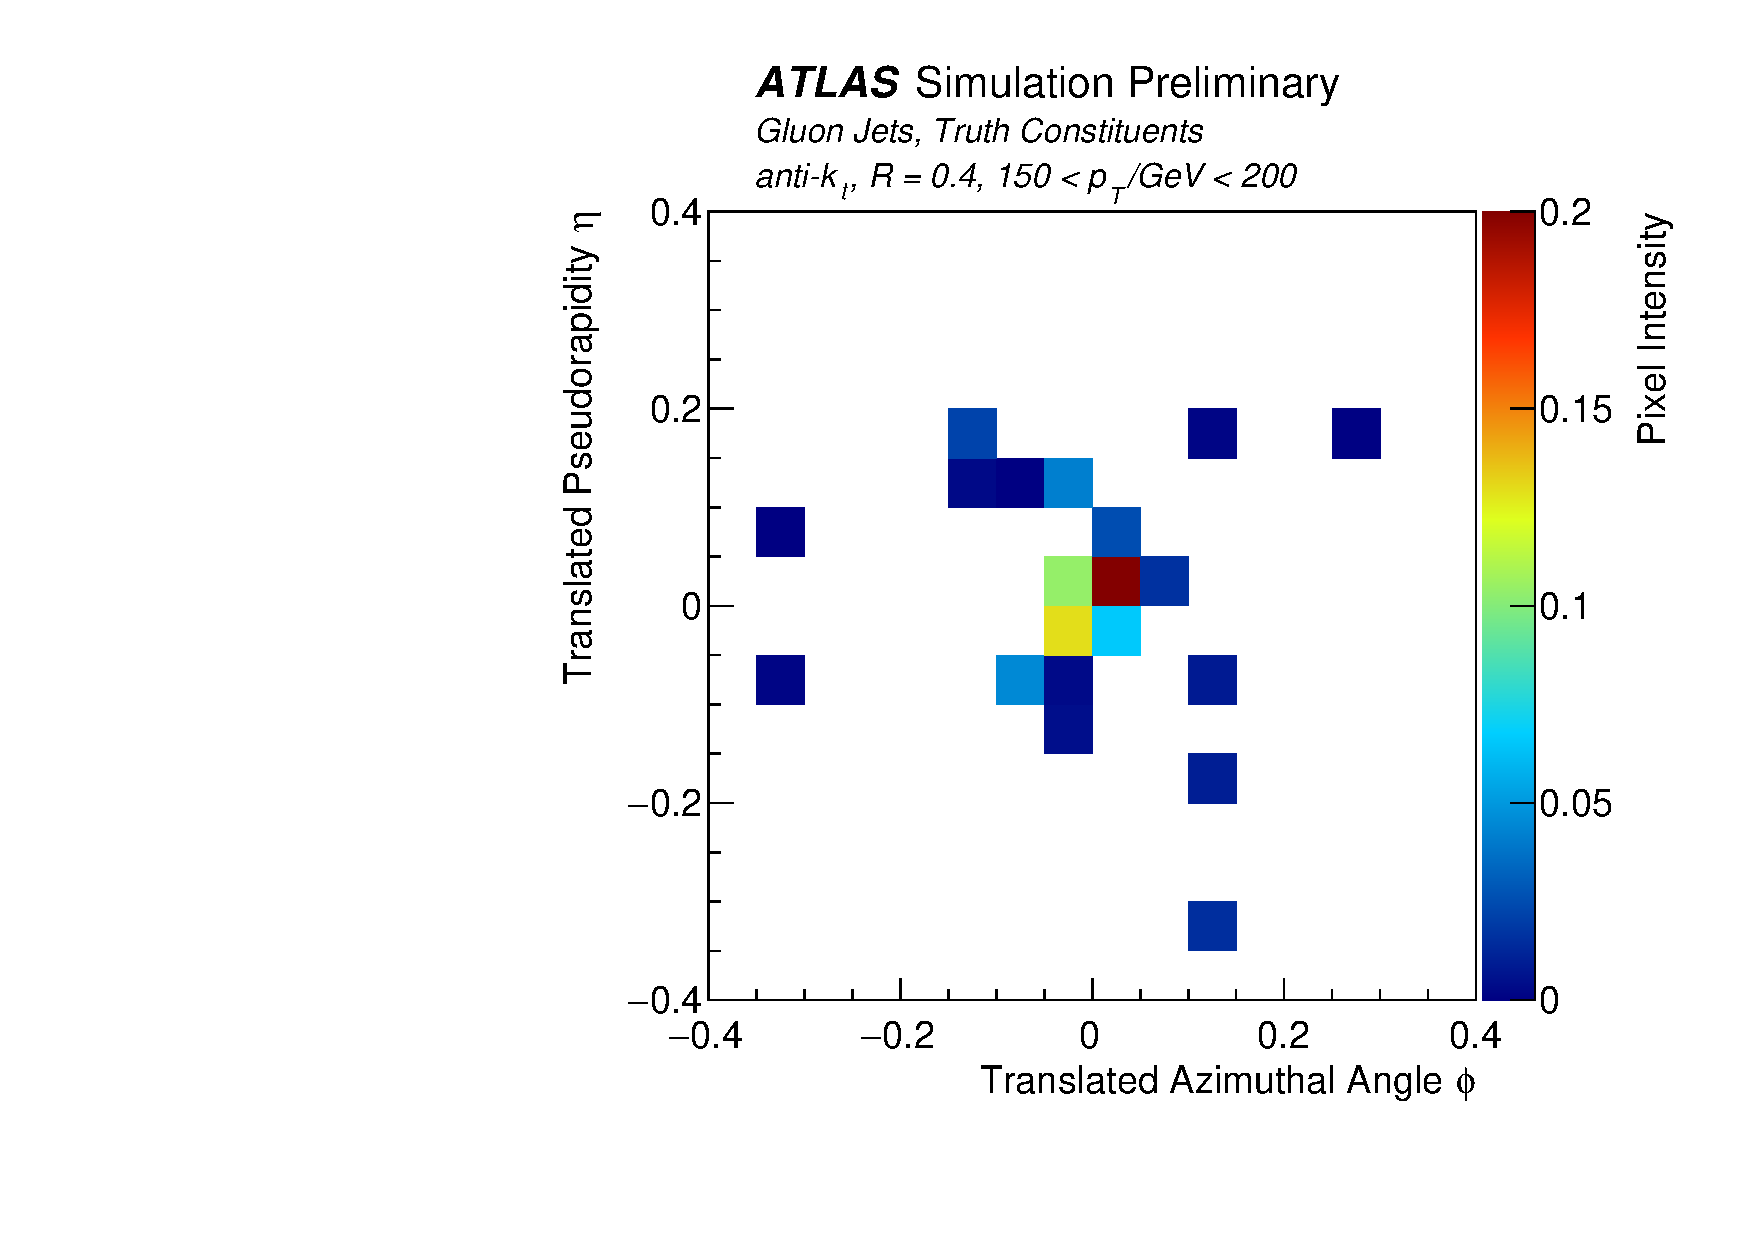
\includegraphics[width=0.45\textwidth]{figures/CNN/gluon_truth_one.pdf}
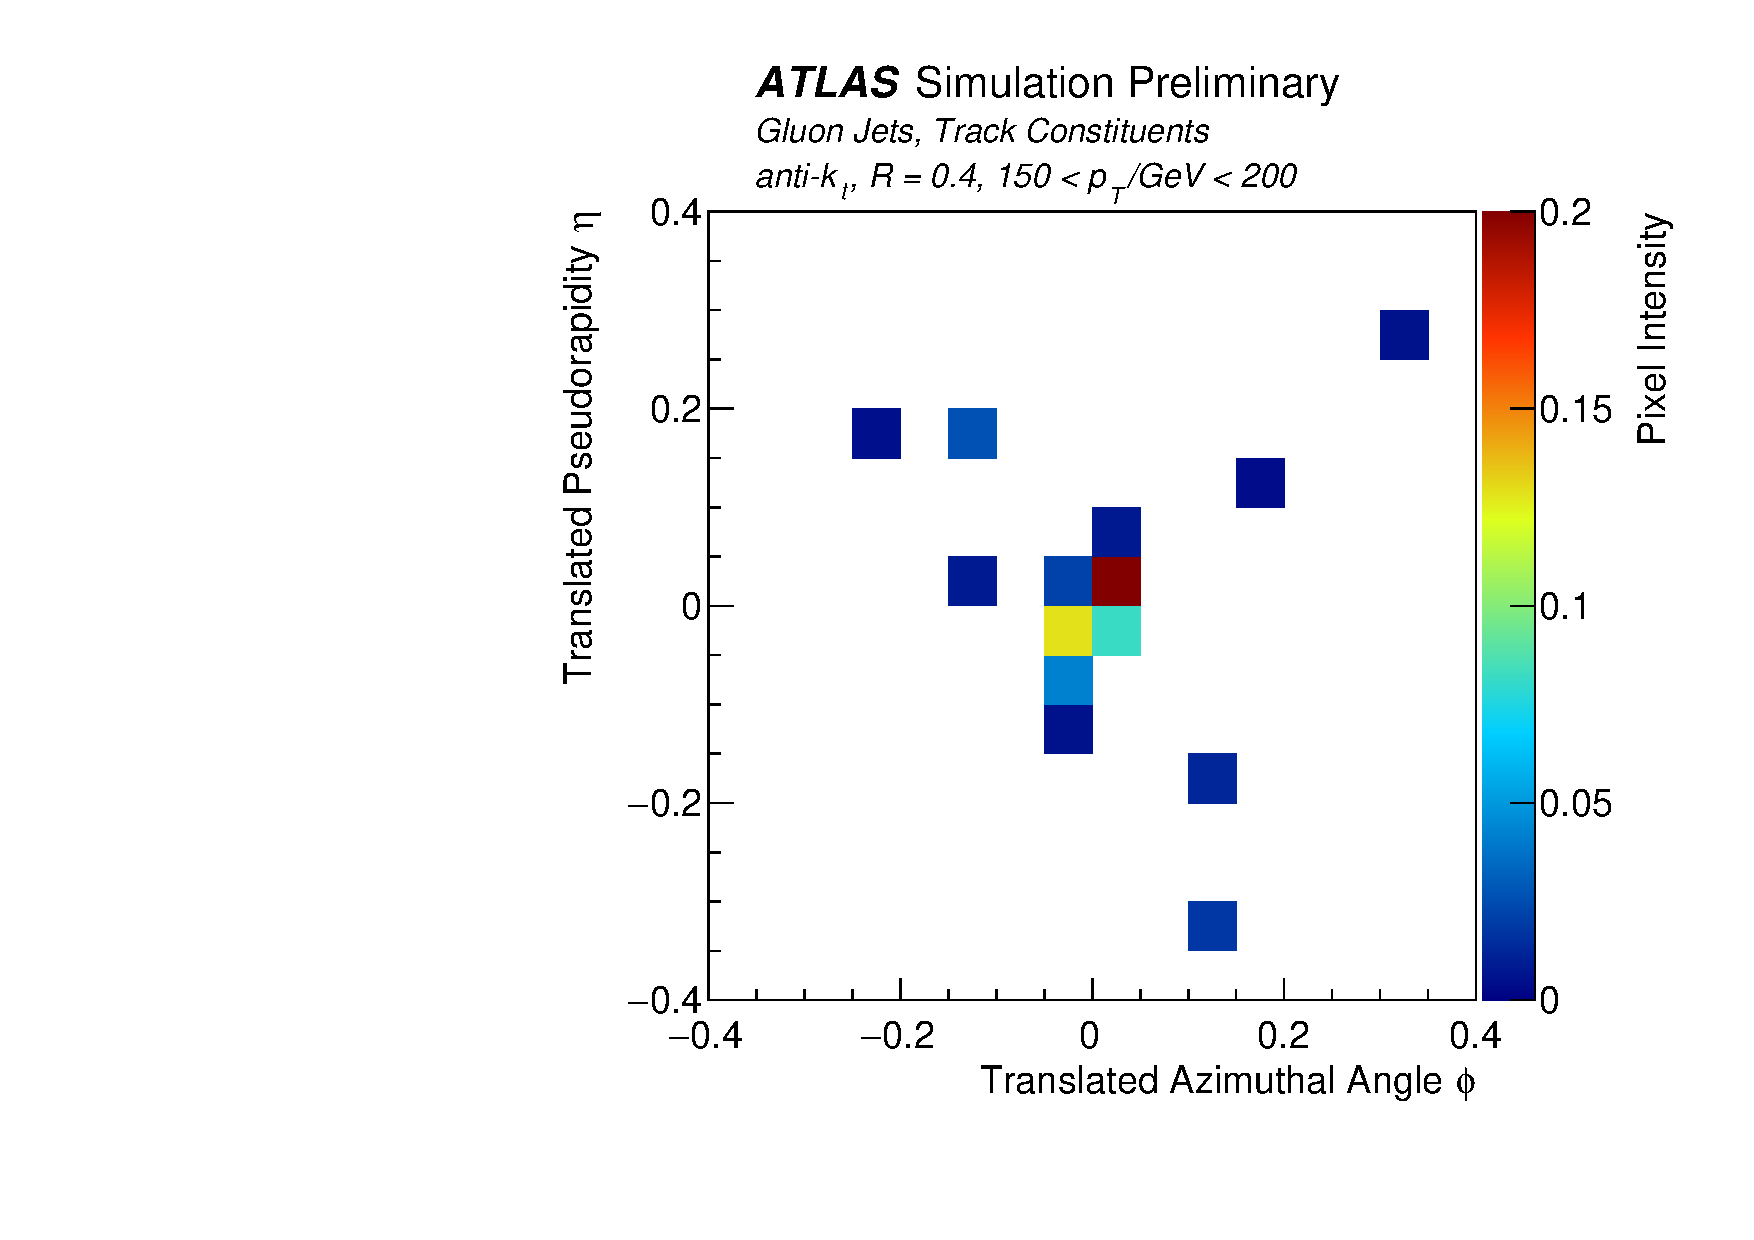
\includegraphics[width=0.45\textwidth]{figures/CNN/gluon_track_one.pdf}\\
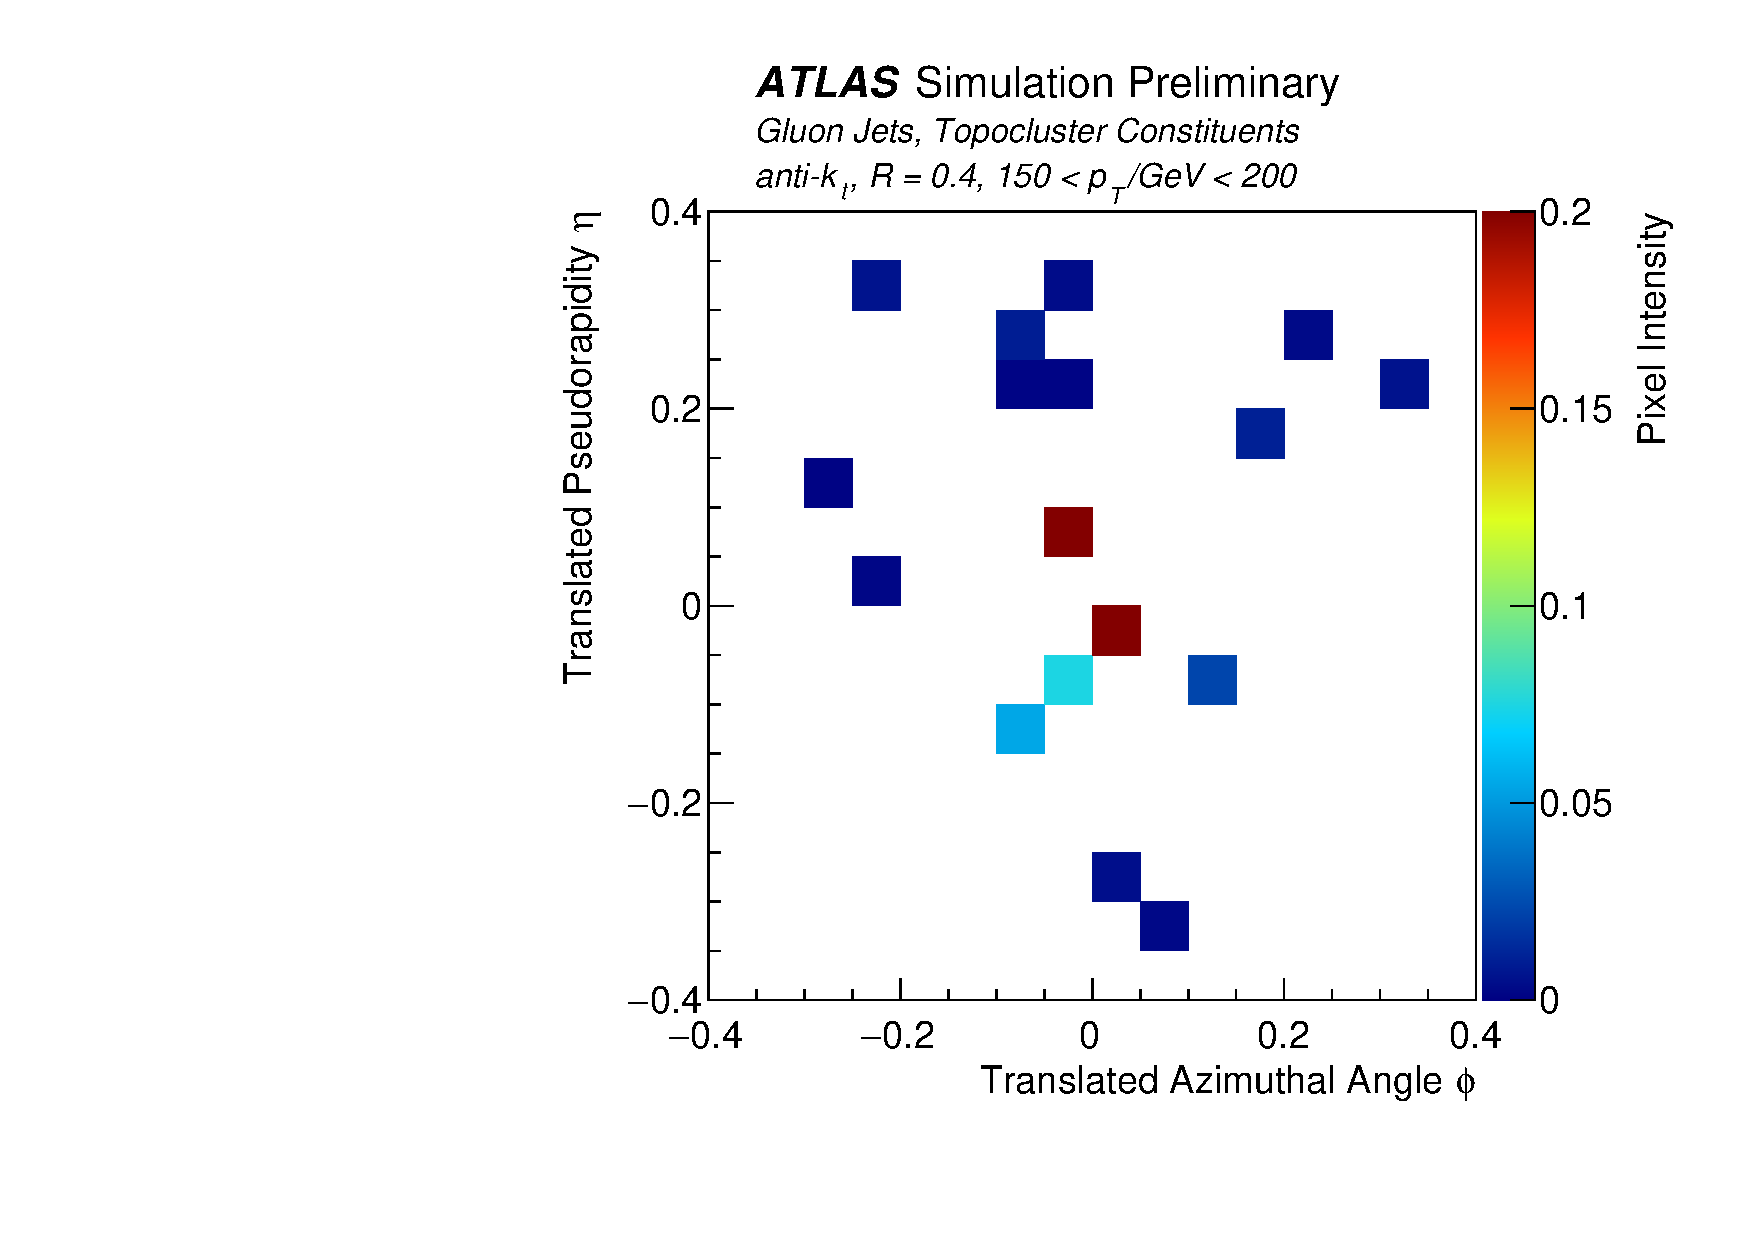
\includegraphics[width=0.45\textwidth]{figures/CNN/gluon_cluster_one.pdf}
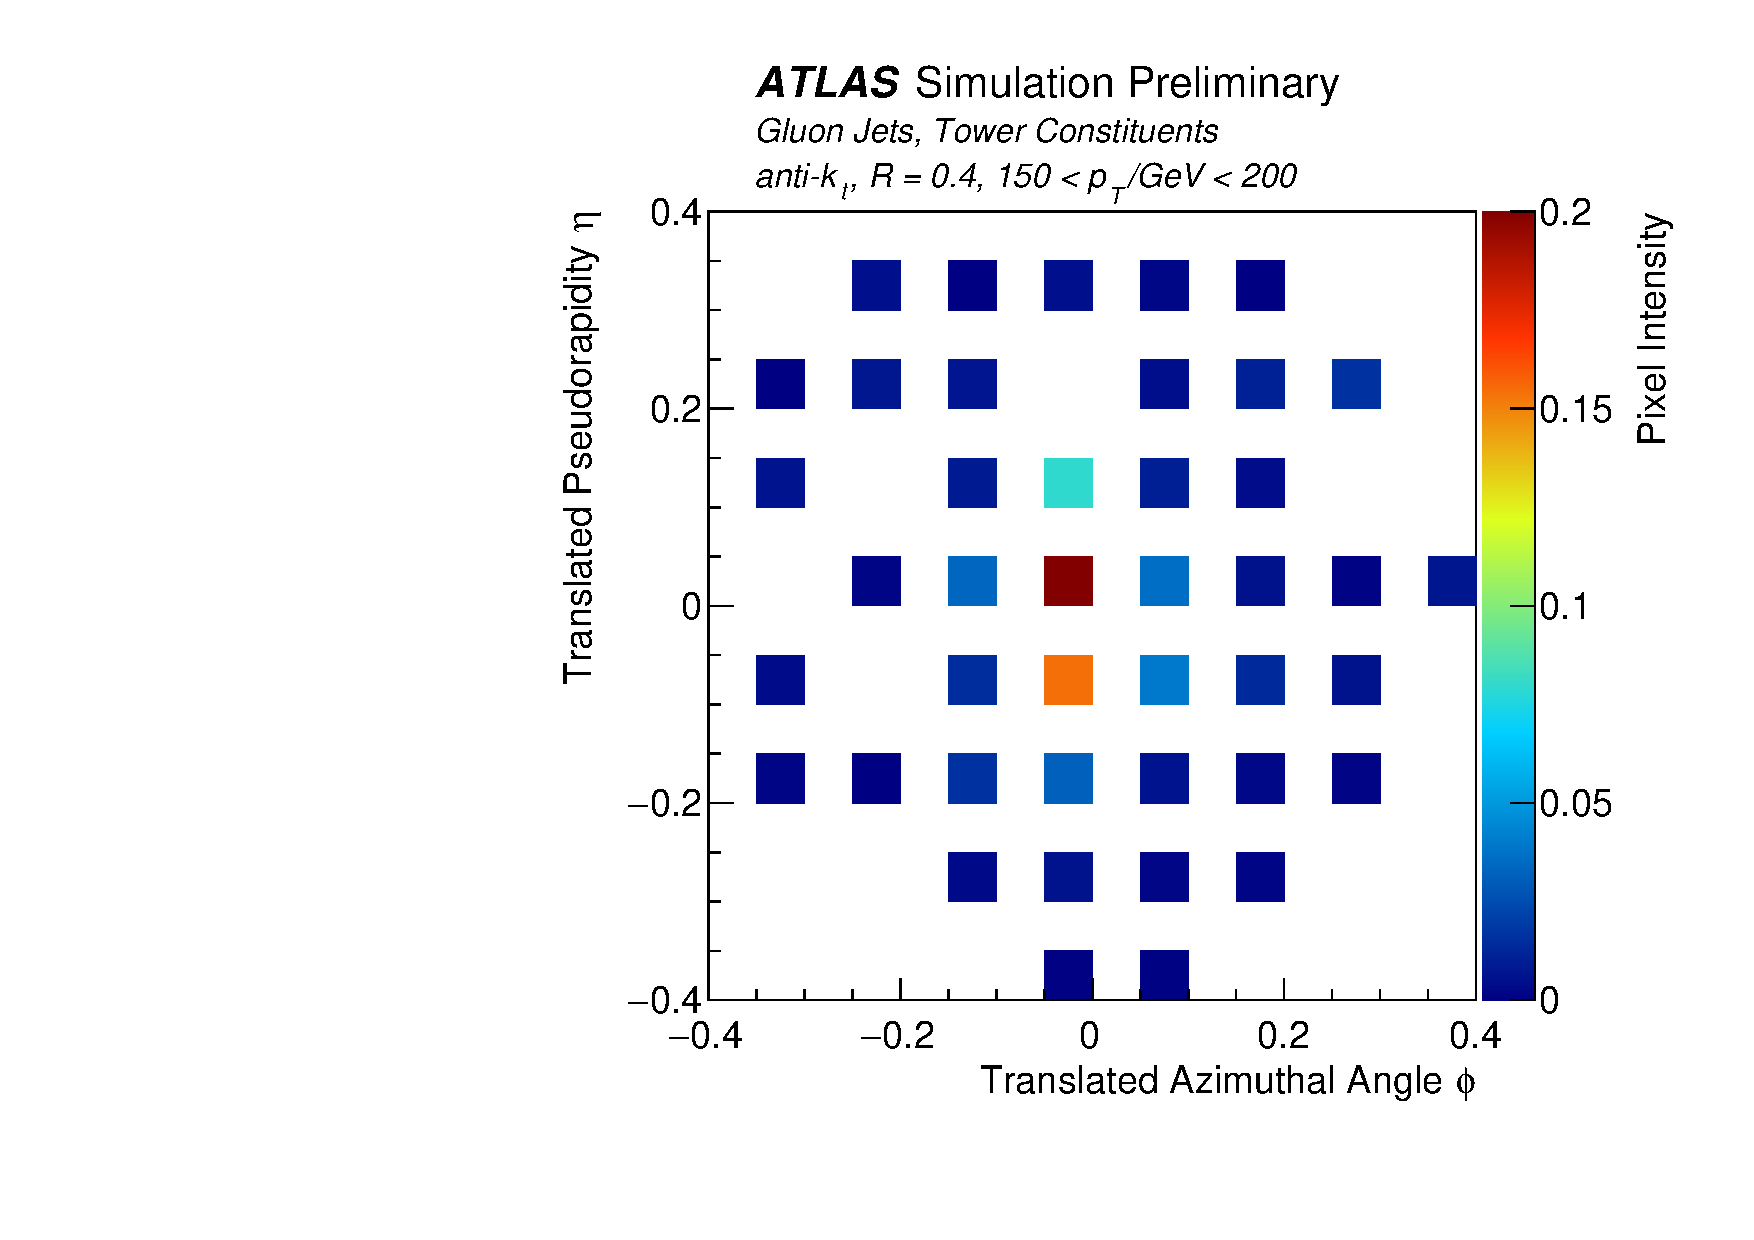
\includegraphics[width=0.45\textwidth]{figures/CNN/gluon_tower_one.pdf}
\caption{The stable particles (top left), track (top right), topocluster (bottom left), and tower (bottom right) images 
for an example gluon jet image.  
The tower image has gaps between hit pixels because the $0.1\times 0.1$ towers are projected onto a $0.05\times 0.05$ jet image.}
\label{fig:cnn-oneimage}
\end{center}
\end{figure}

\begin{figure}[htpb]
\begin{center}
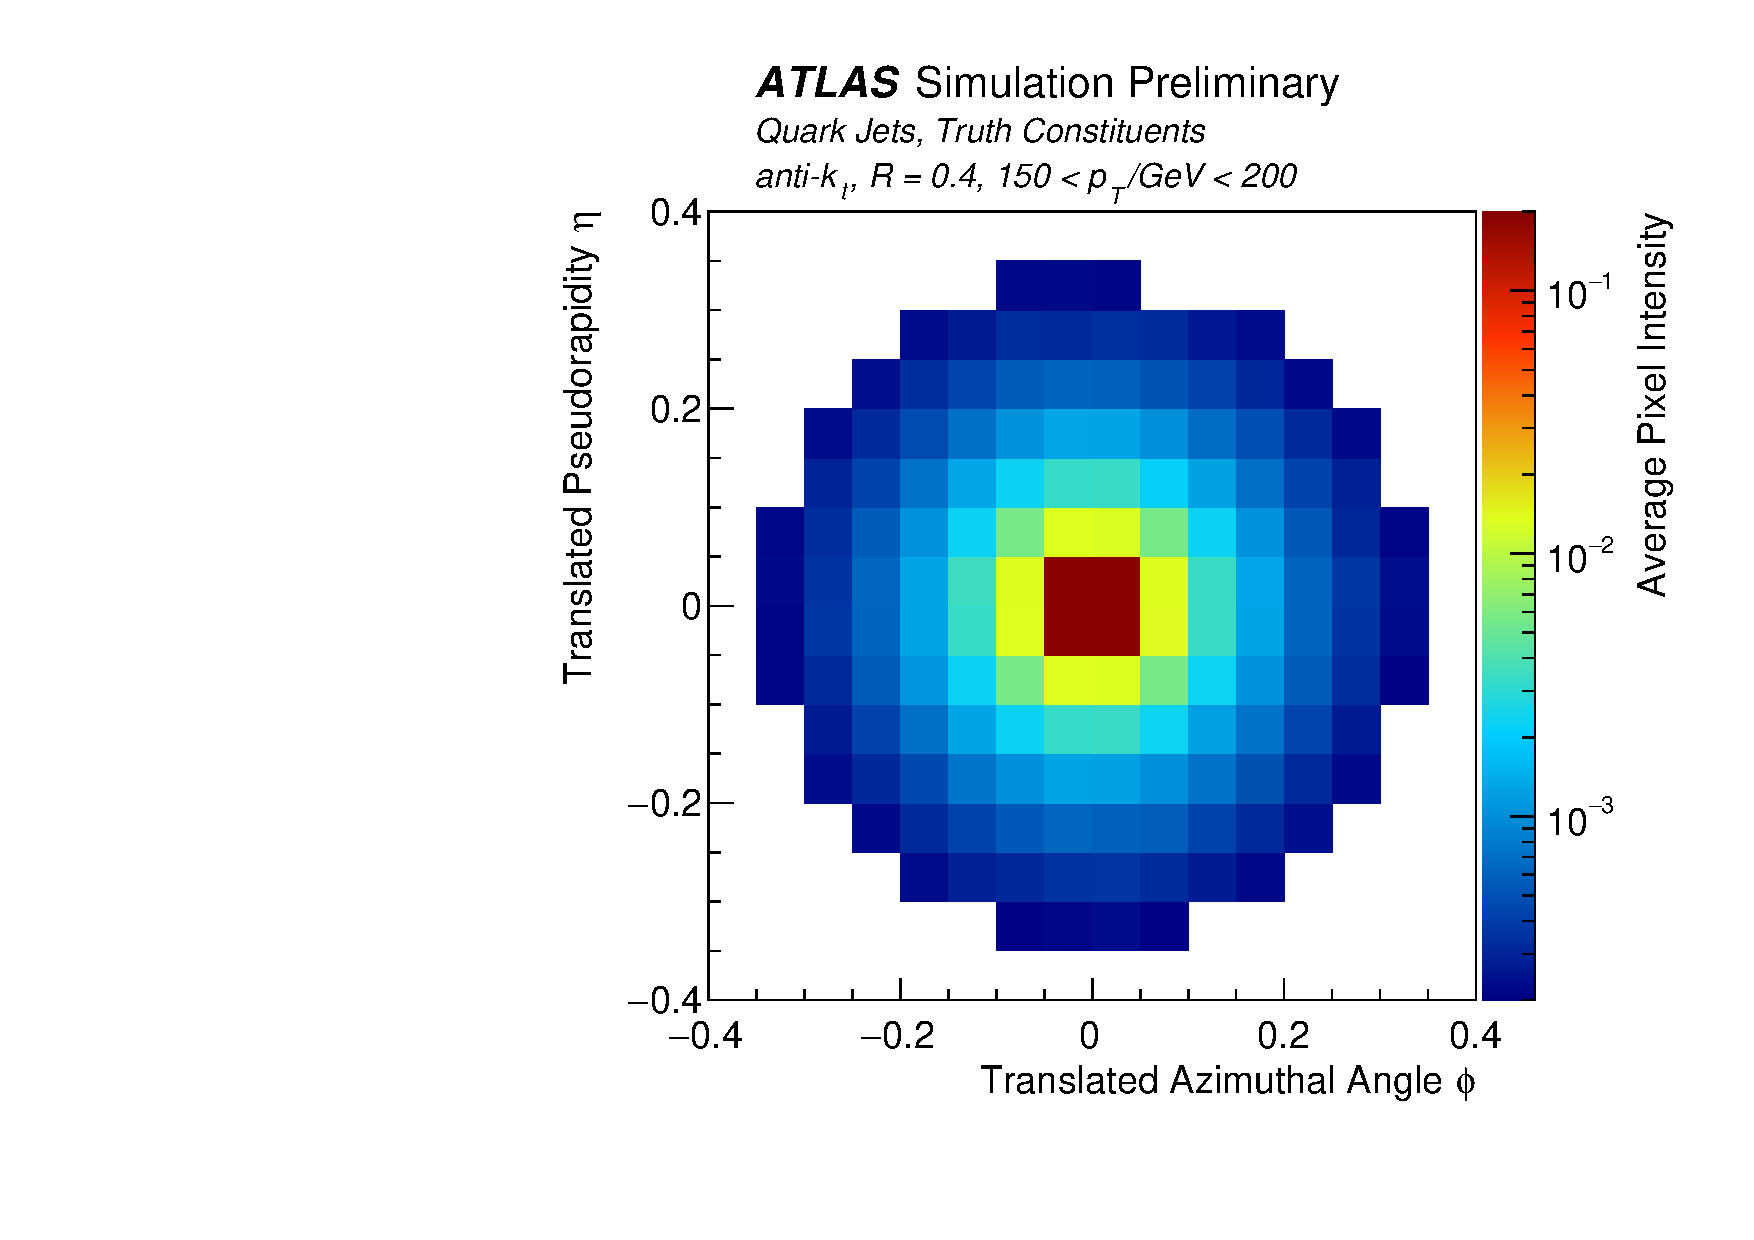
\includegraphics[width=0.31\textwidth]{figures/CNN/quark_truth.pdf}
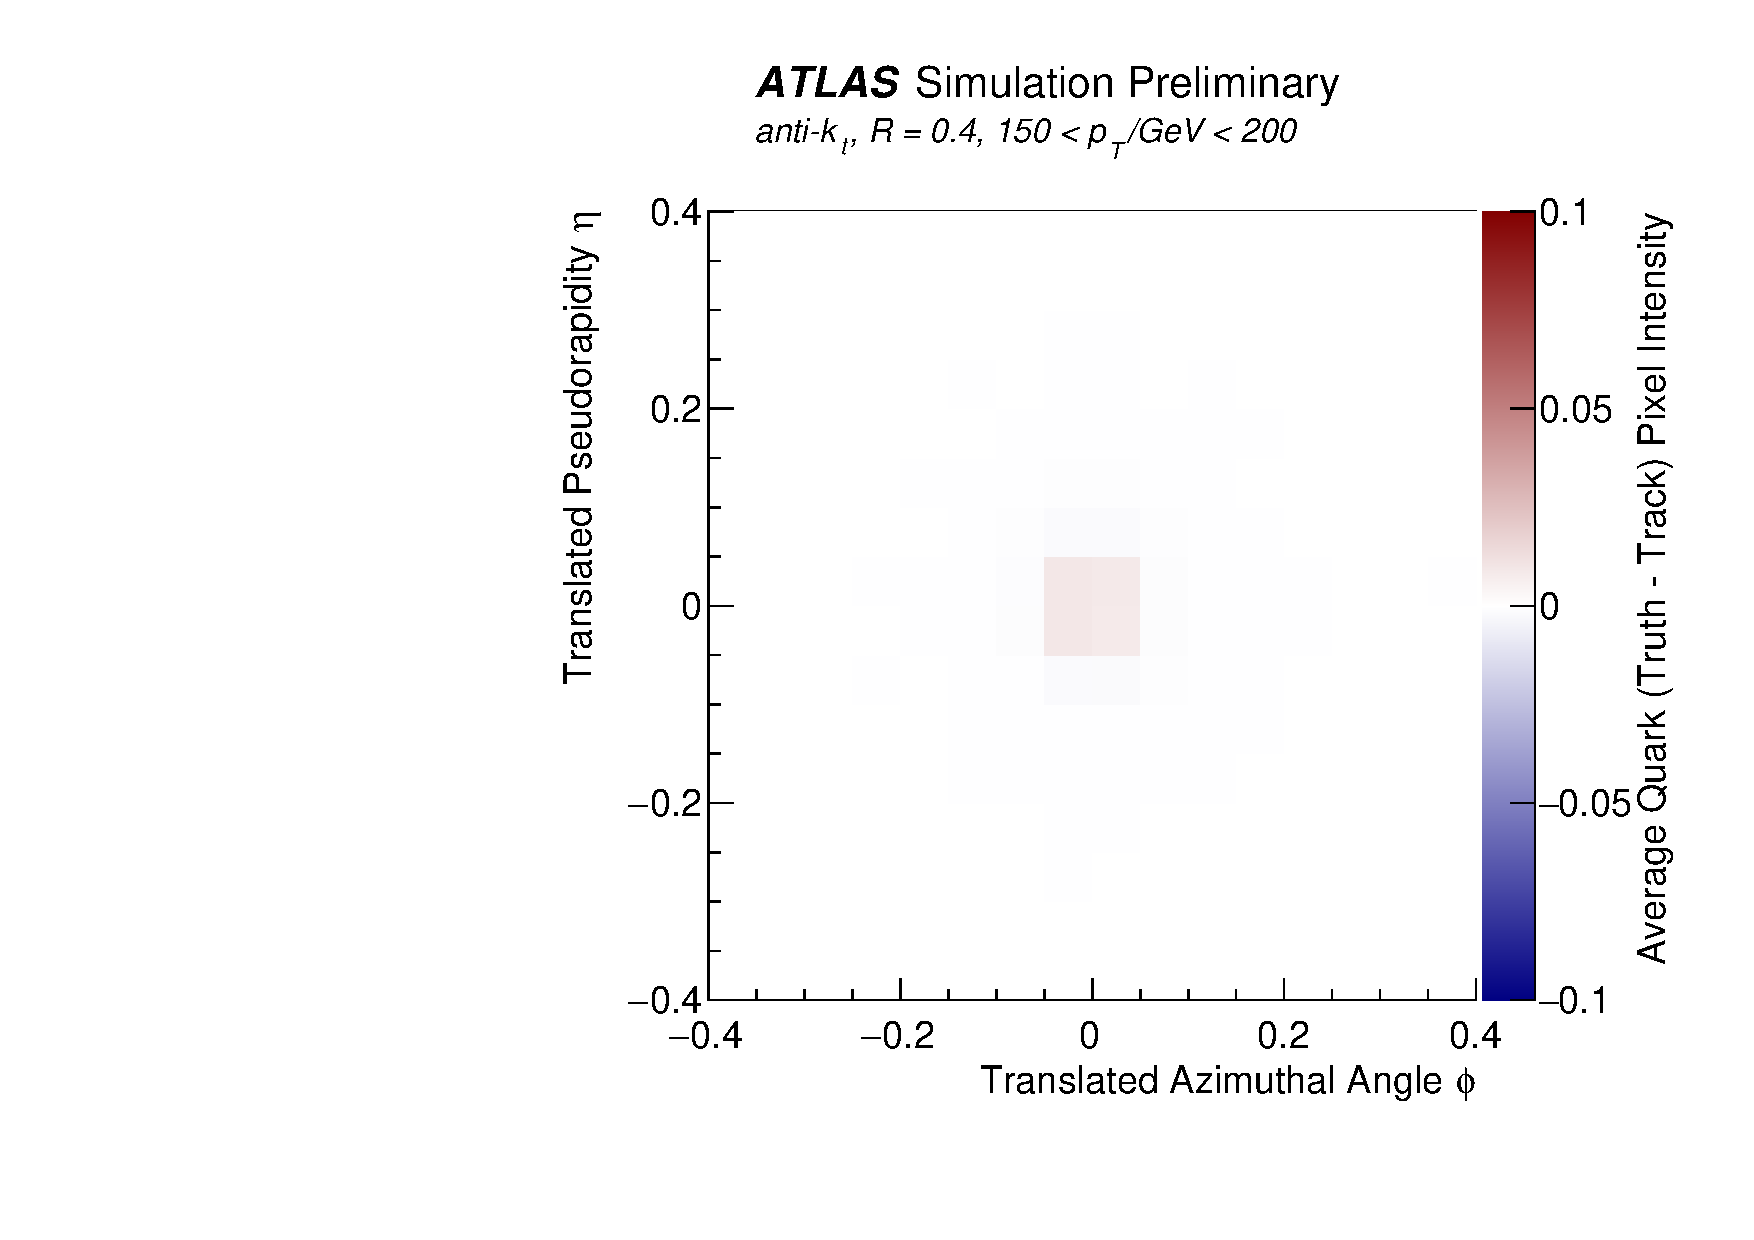
\includegraphics[width=0.31\textwidth]{figures/CNN/diff_quark_truth_track.pdf}
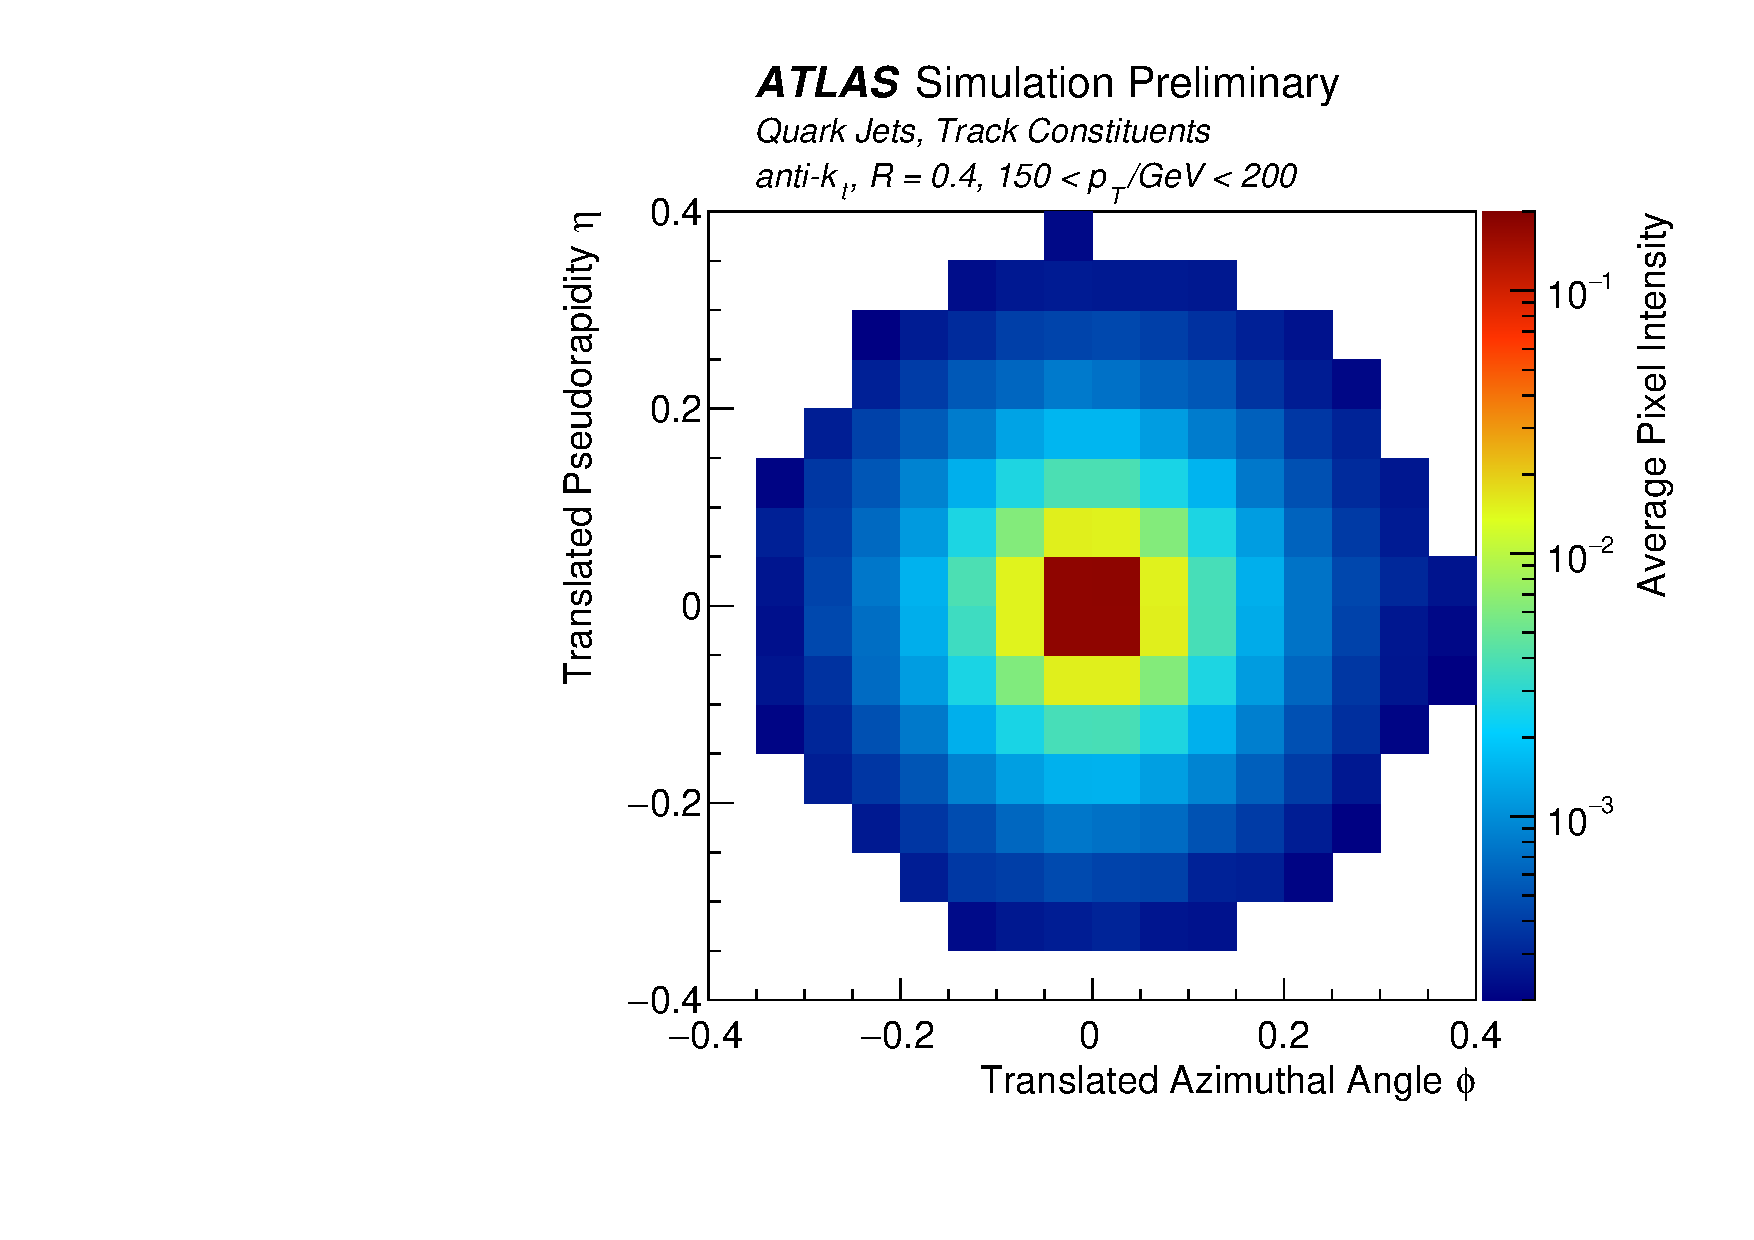
\includegraphics[width=0.31\textwidth]{figures/CNN/quark_track.pdf}\\
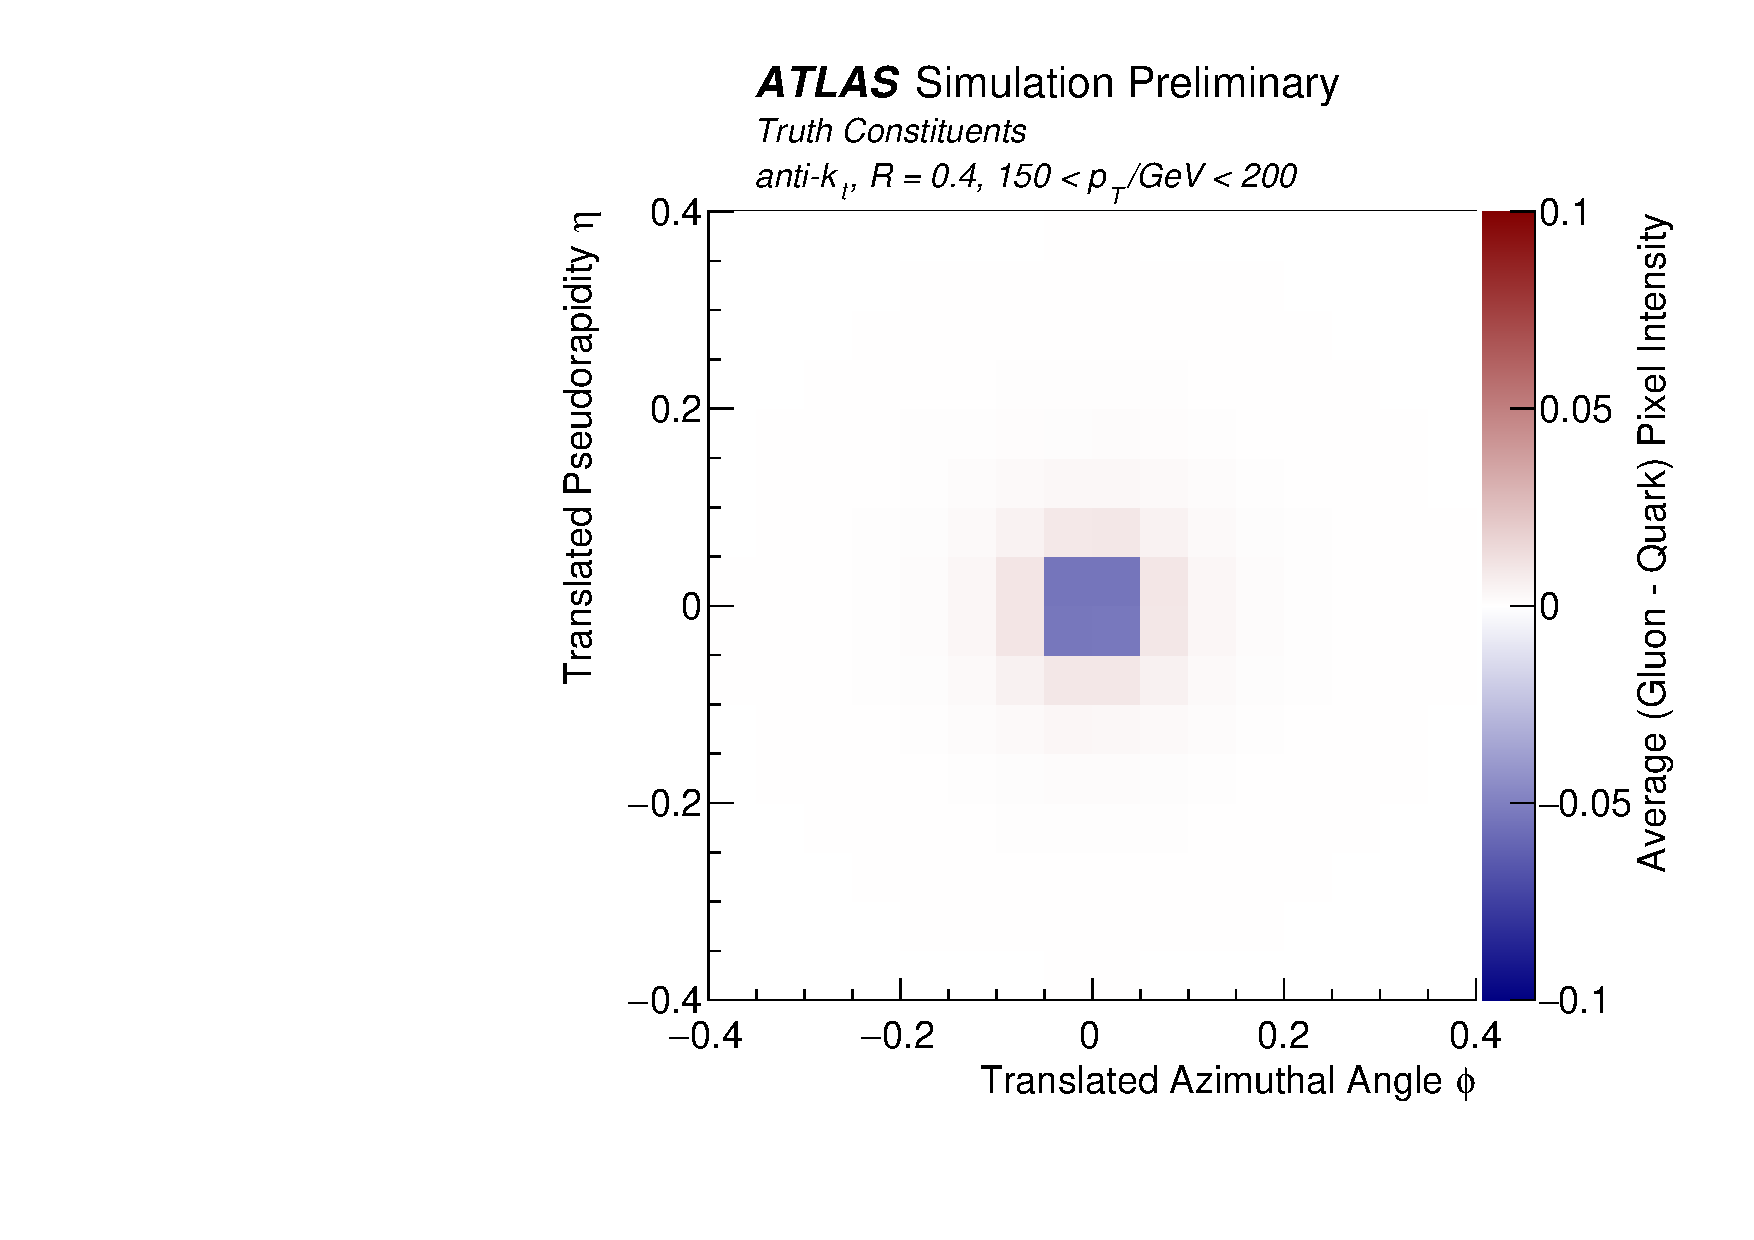
\includegraphics[width=0.31\textwidth]{figures/CNN/diff_truth.pdf}\hspace{54mm}
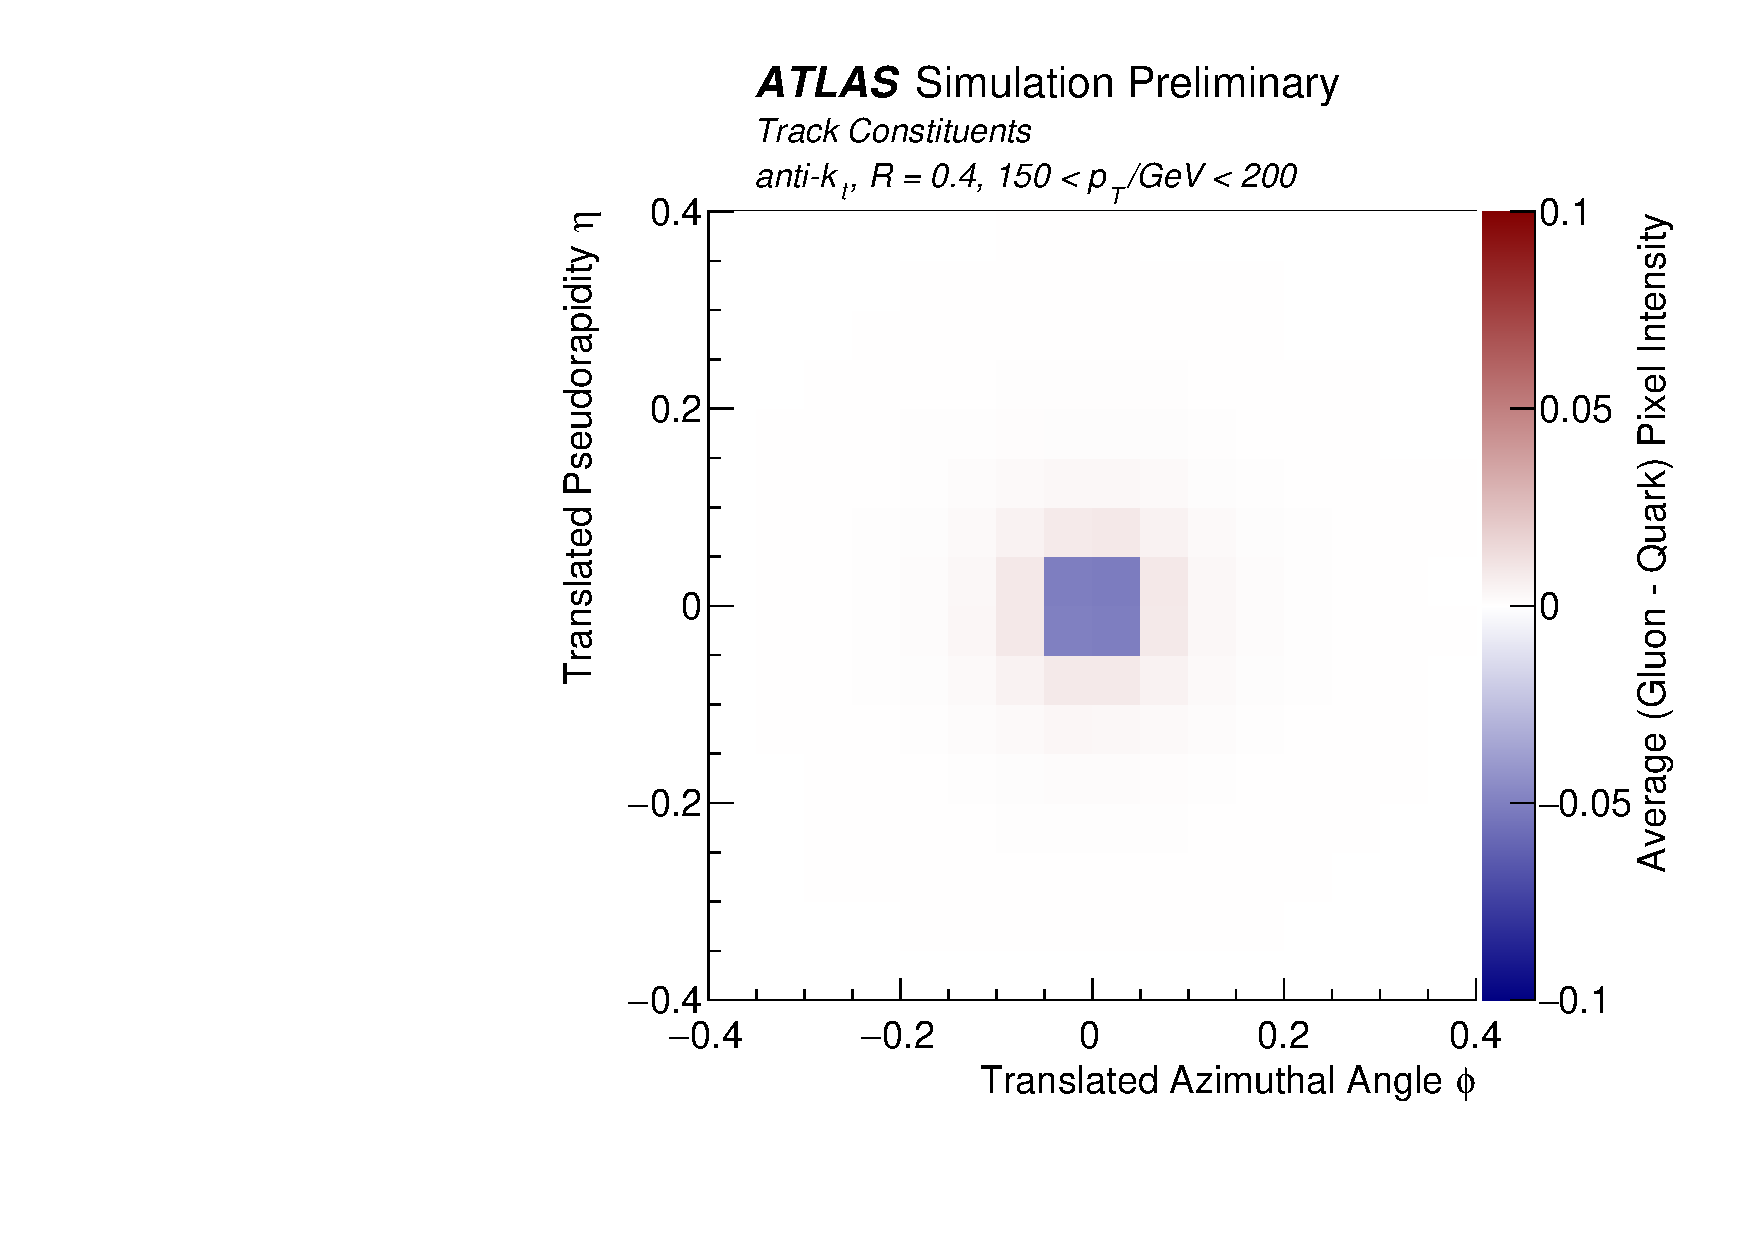
\includegraphics[width=0.31\textwidth]{figures/CNN/diff_track.pdf}\\
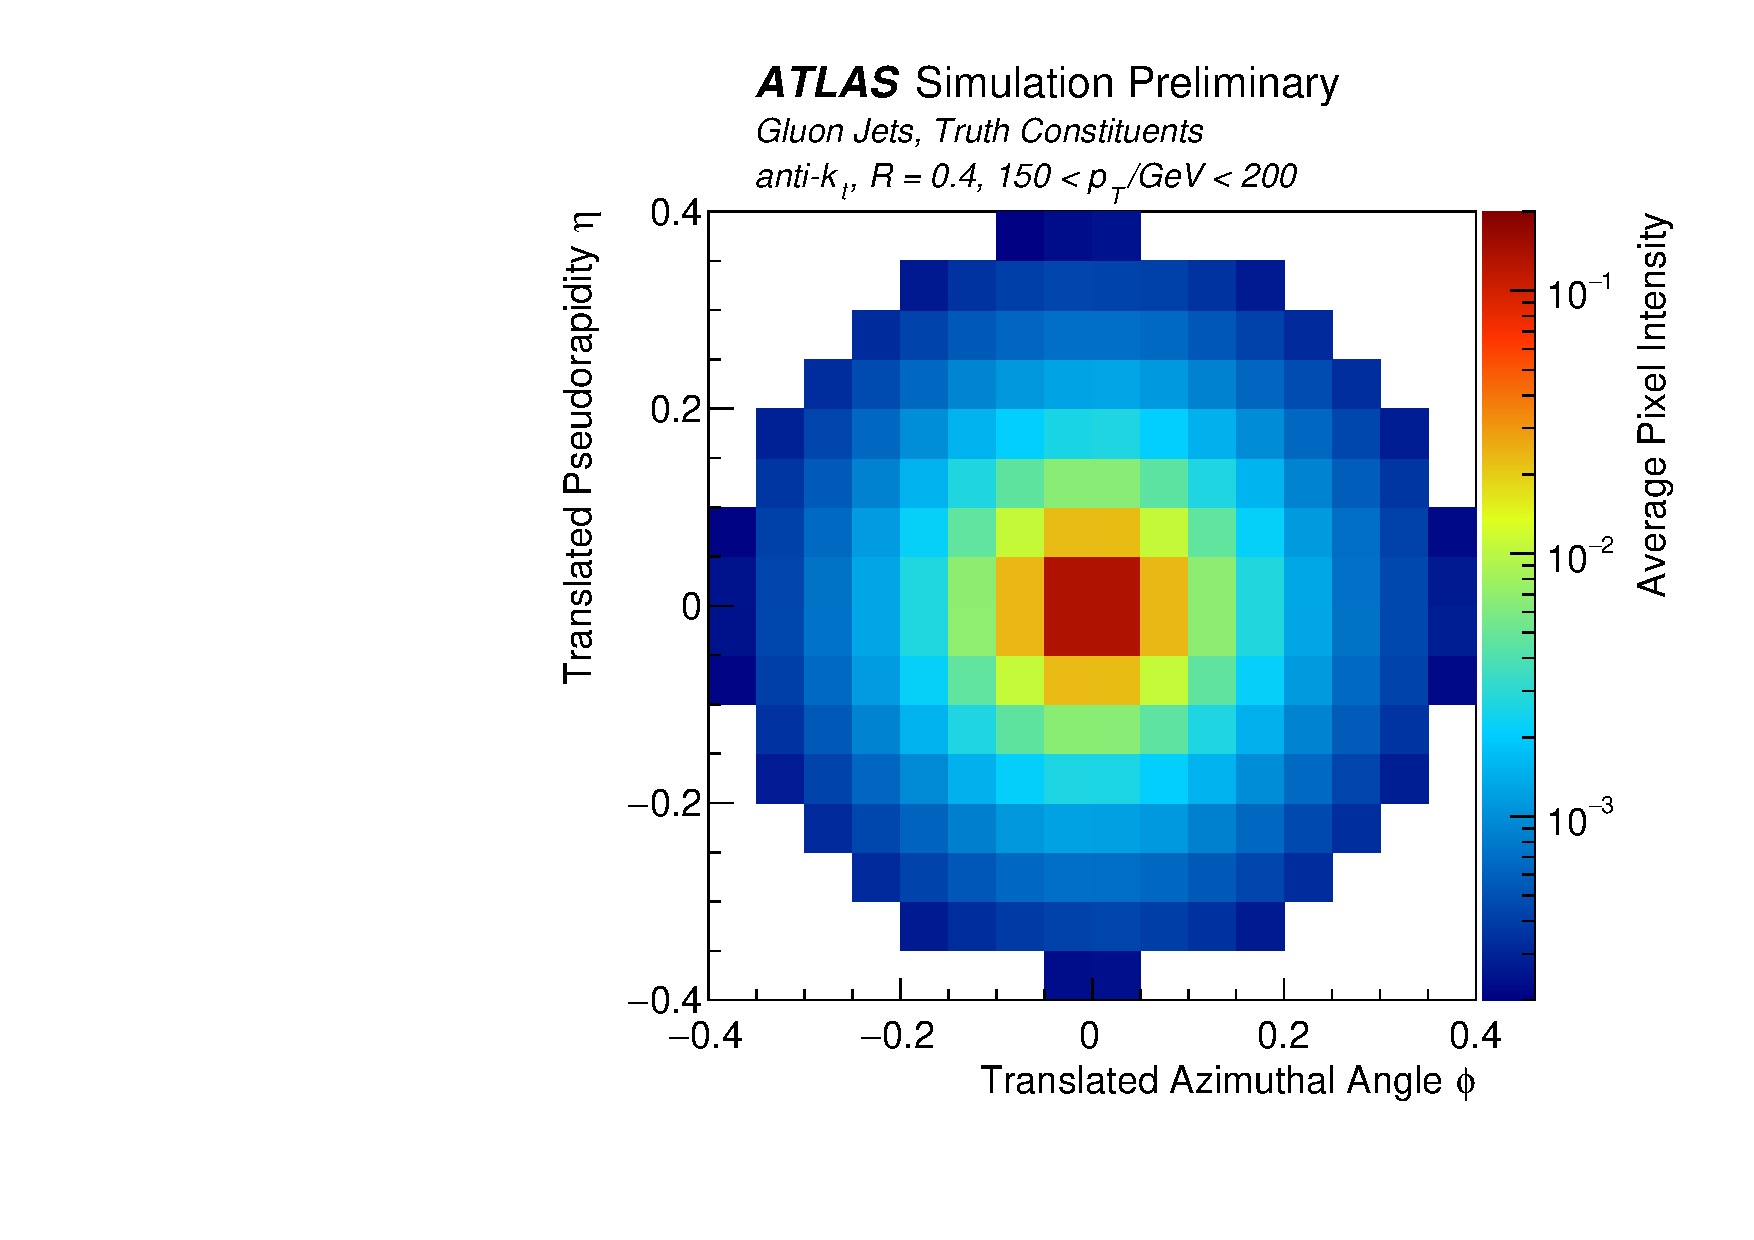
\includegraphics[width=0.31\textwidth]{figures/CNN/gluon_truth.pdf}
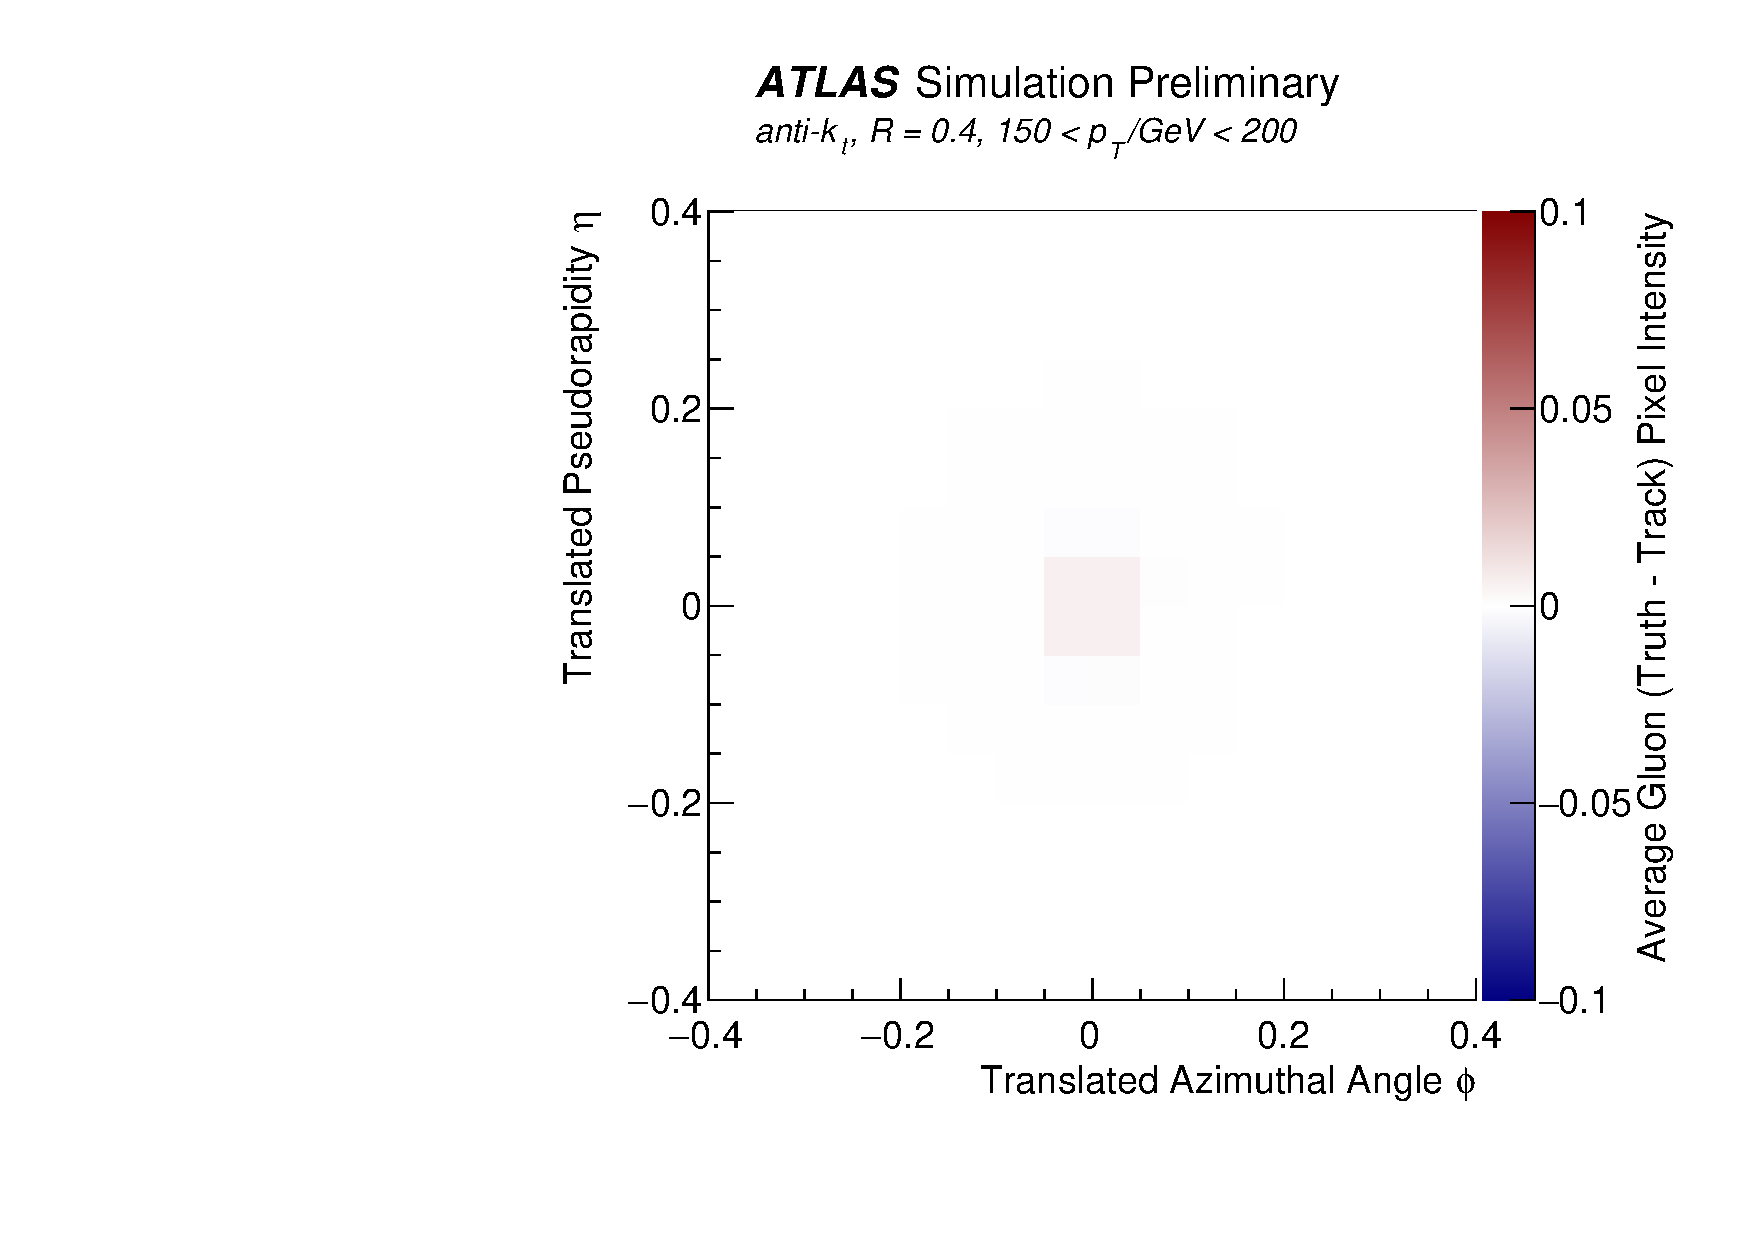
\includegraphics[width=0.31\textwidth]{figures/CNN/diff_gluon_truth_track.pdf}
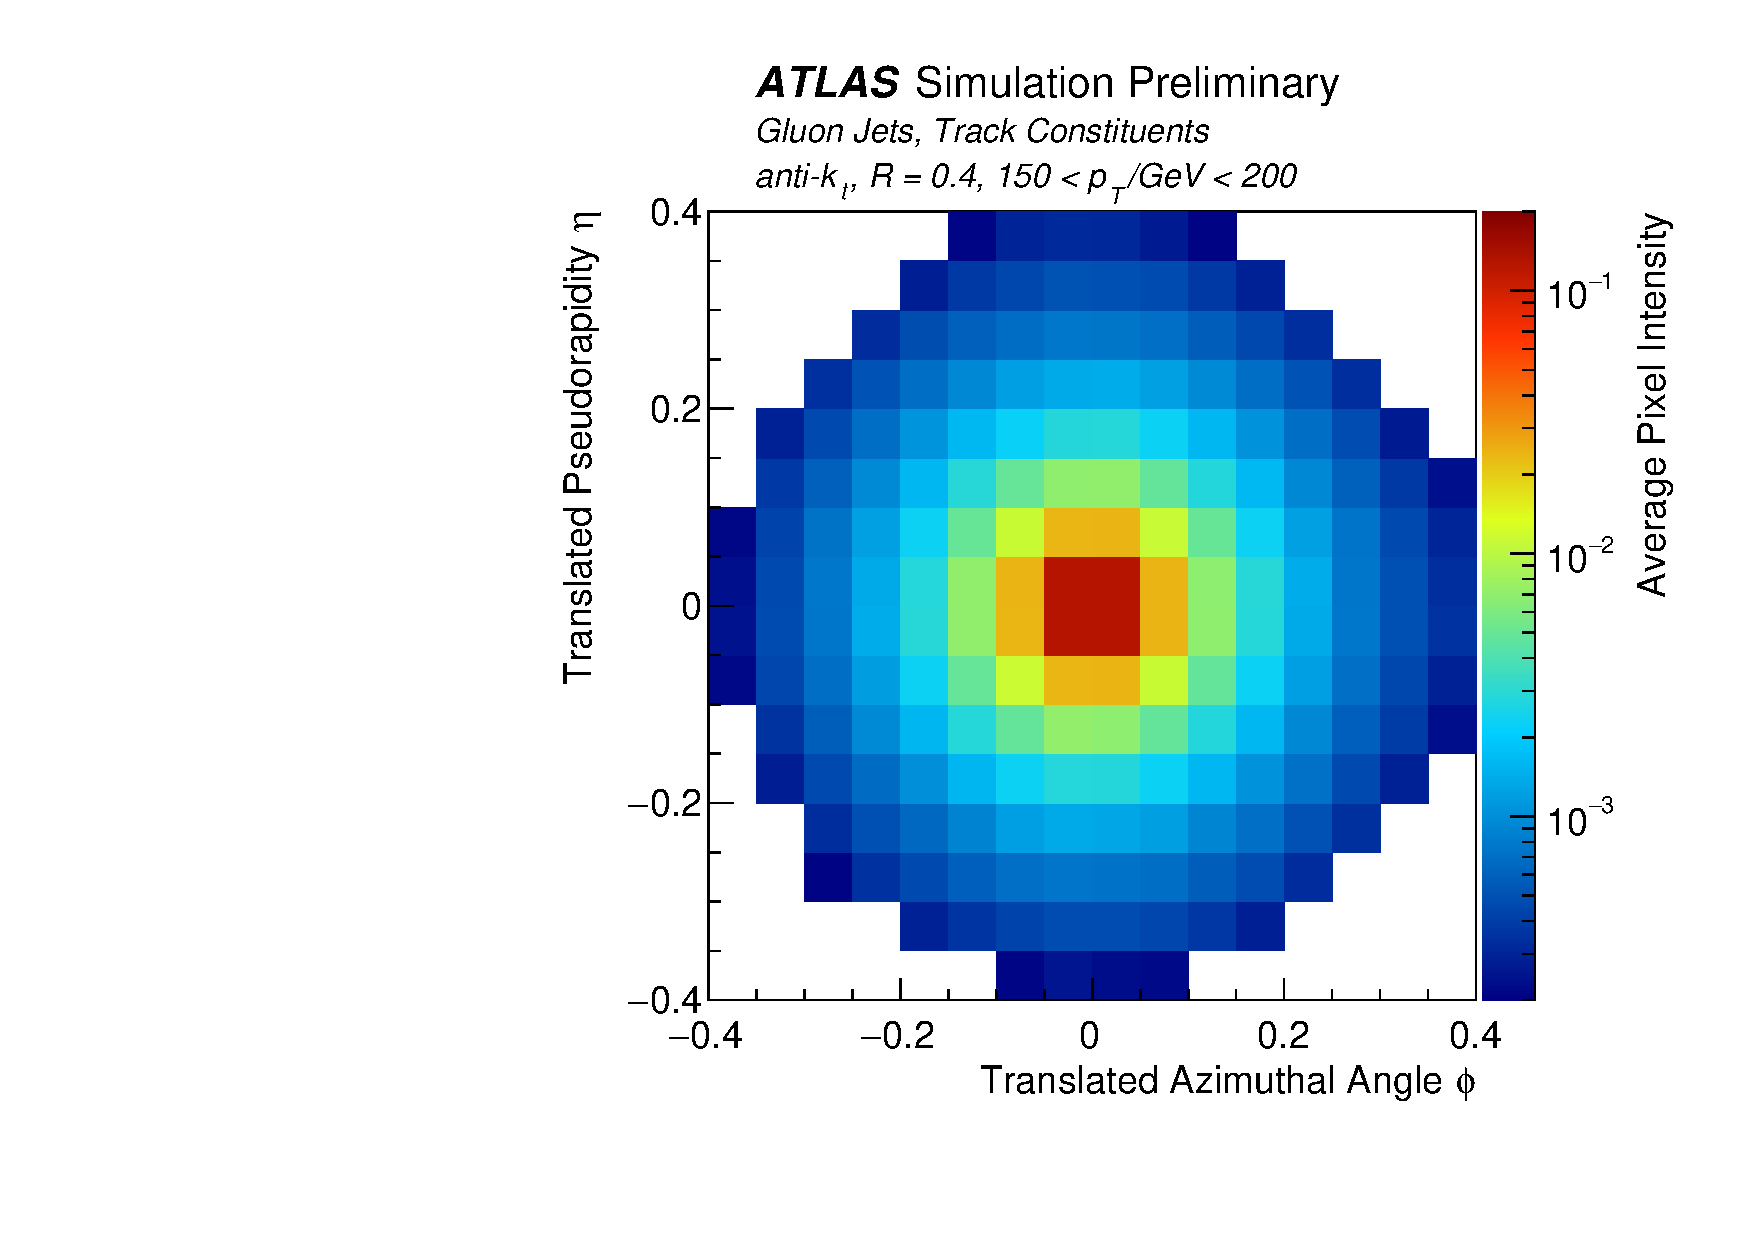
\includegraphics[width=0.31\textwidth]{figures/CNN/gluon_track.pdf}
\caption{The four corners show the average quark (upper) and gluon (lower) jet images, from true constituents, both charged and neutral, (left) and reconstructed tracks (right); the four plots on the edges show the difference between the adjacent plots, for example the top plot shows the difference between the average quark jet for stable particles and reconstructed tracks. Quark-jets are more collimated than gluon ones, and track images show slightly less central activity than in the true jet.}
\label{fig:cnn-avg:truthtrack}
\end{center}
\end{figure}

\begin{figure}[h!]
\begin{center}
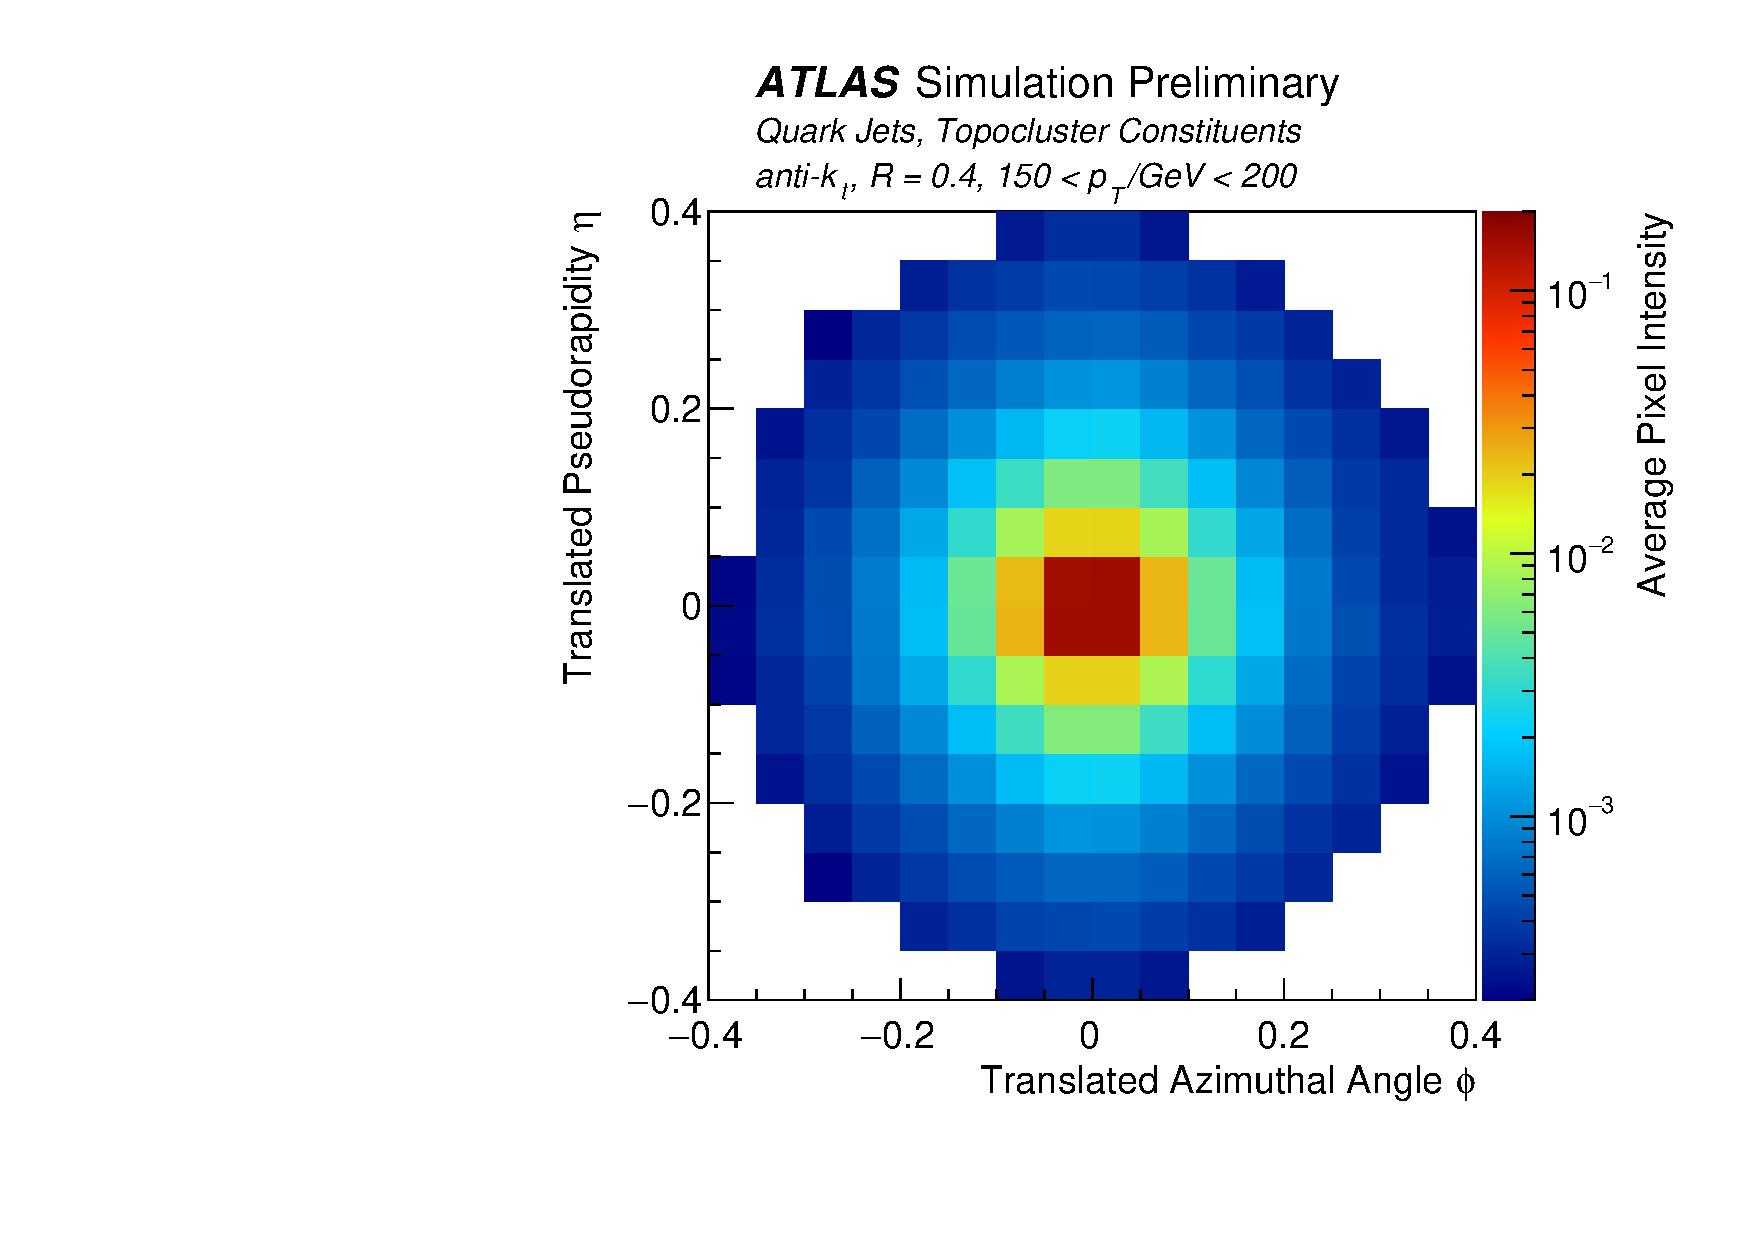
\includegraphics[width=0.31\textwidth]{figures/CNN/quark_cluster.pdf}
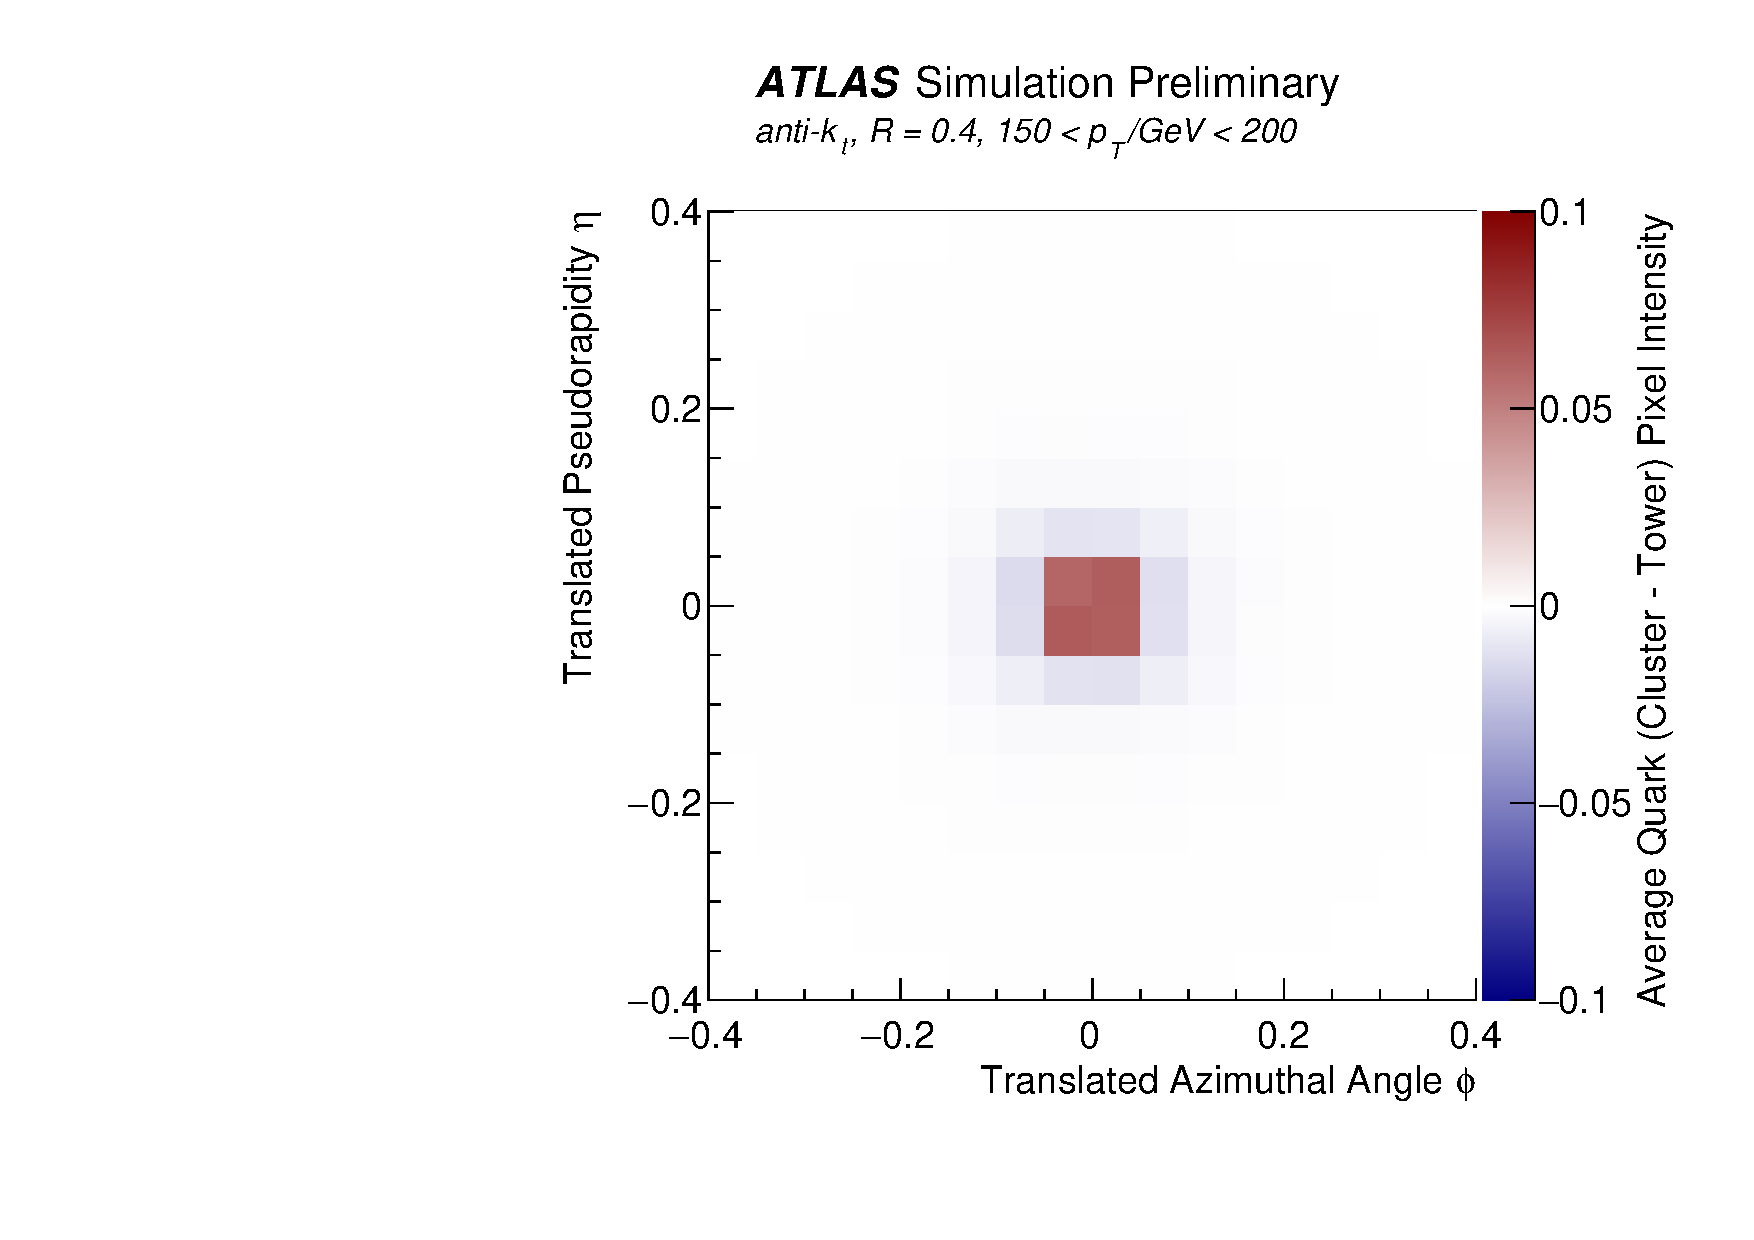
\includegraphics[width=0.31\textwidth]{figures/CNN/diff_quark_cluster_tower.pdf}
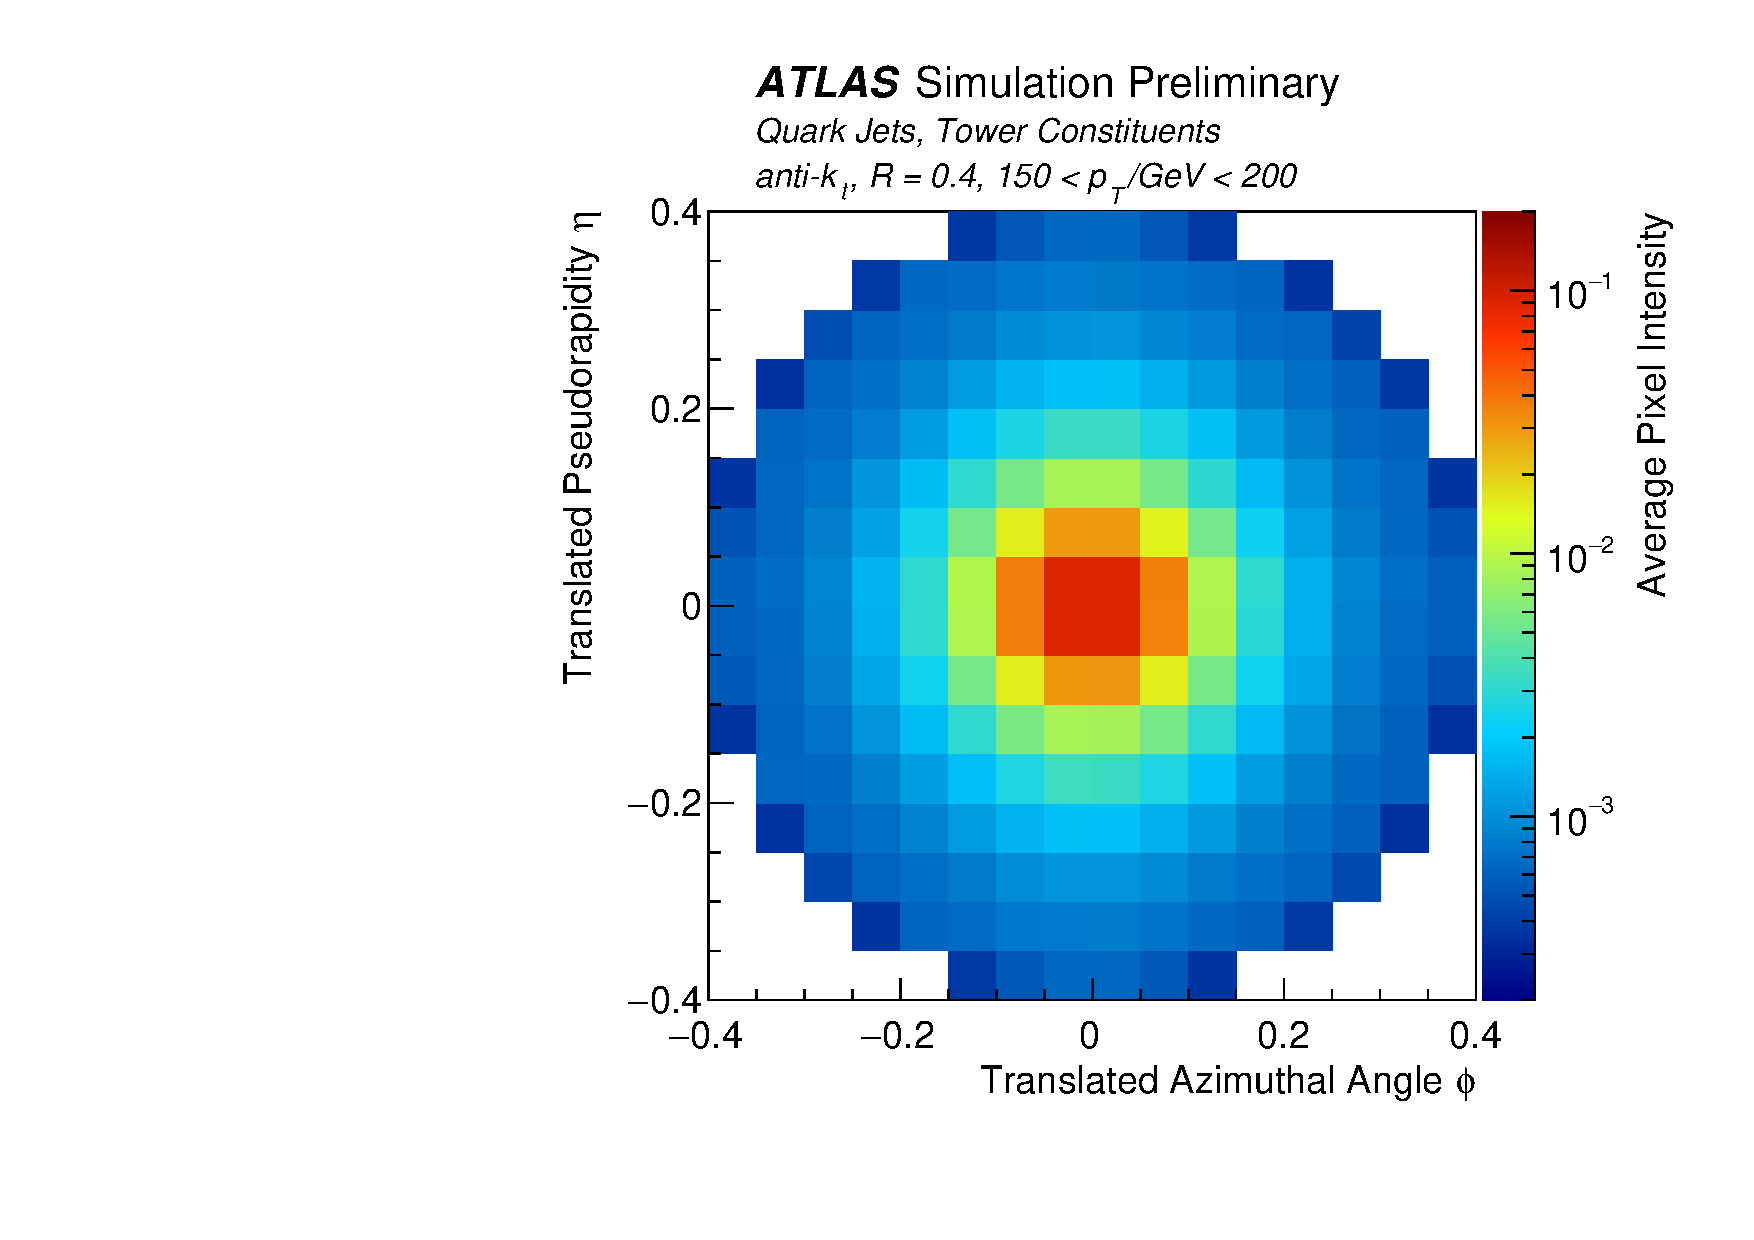
\includegraphics[width=0.31\textwidth]{figures/CNN/quark_tower.pdf}\\
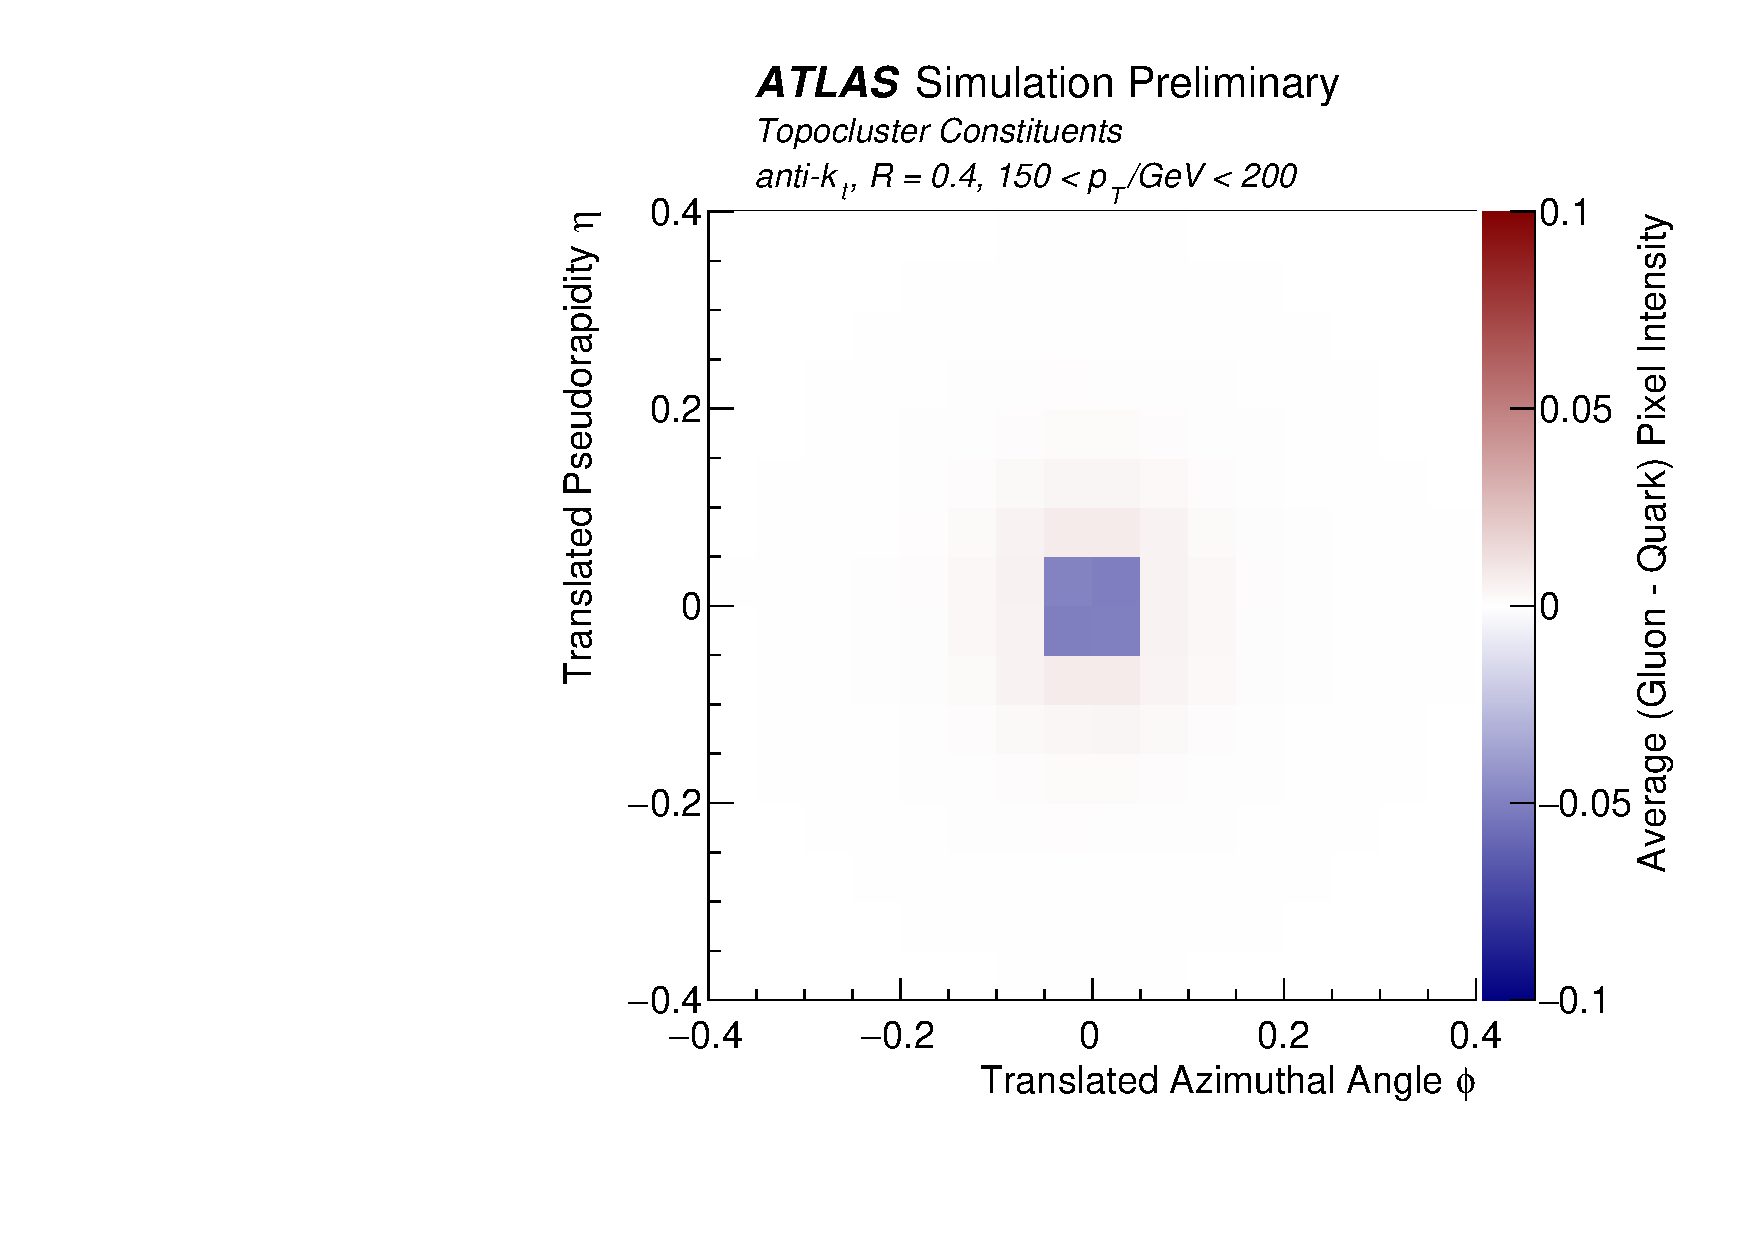
\includegraphics[width=0.31\textwidth]{figures/CNN/diff_cluster.pdf}\hspace{54mm}
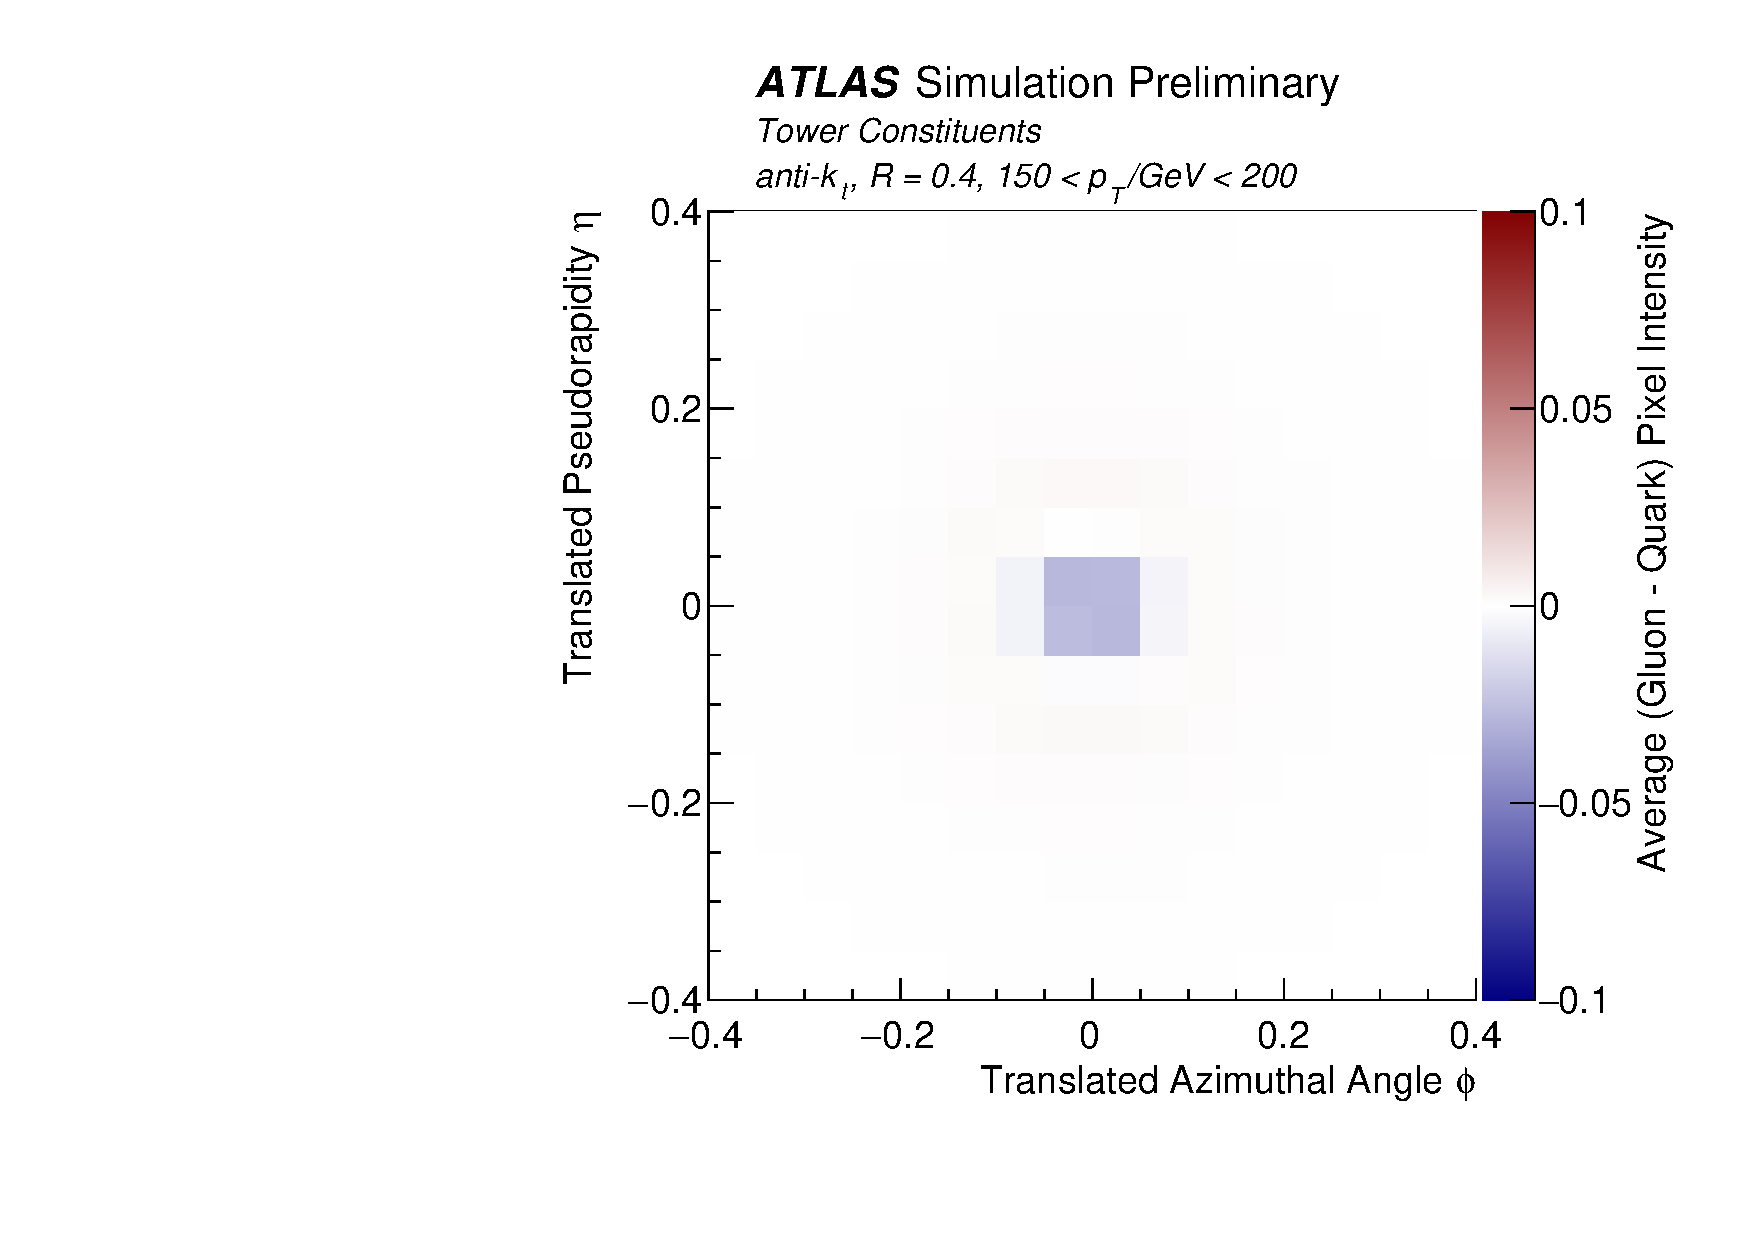
\includegraphics[width=0.31\textwidth]{figures/CNN/diff_tower.pdf}\\
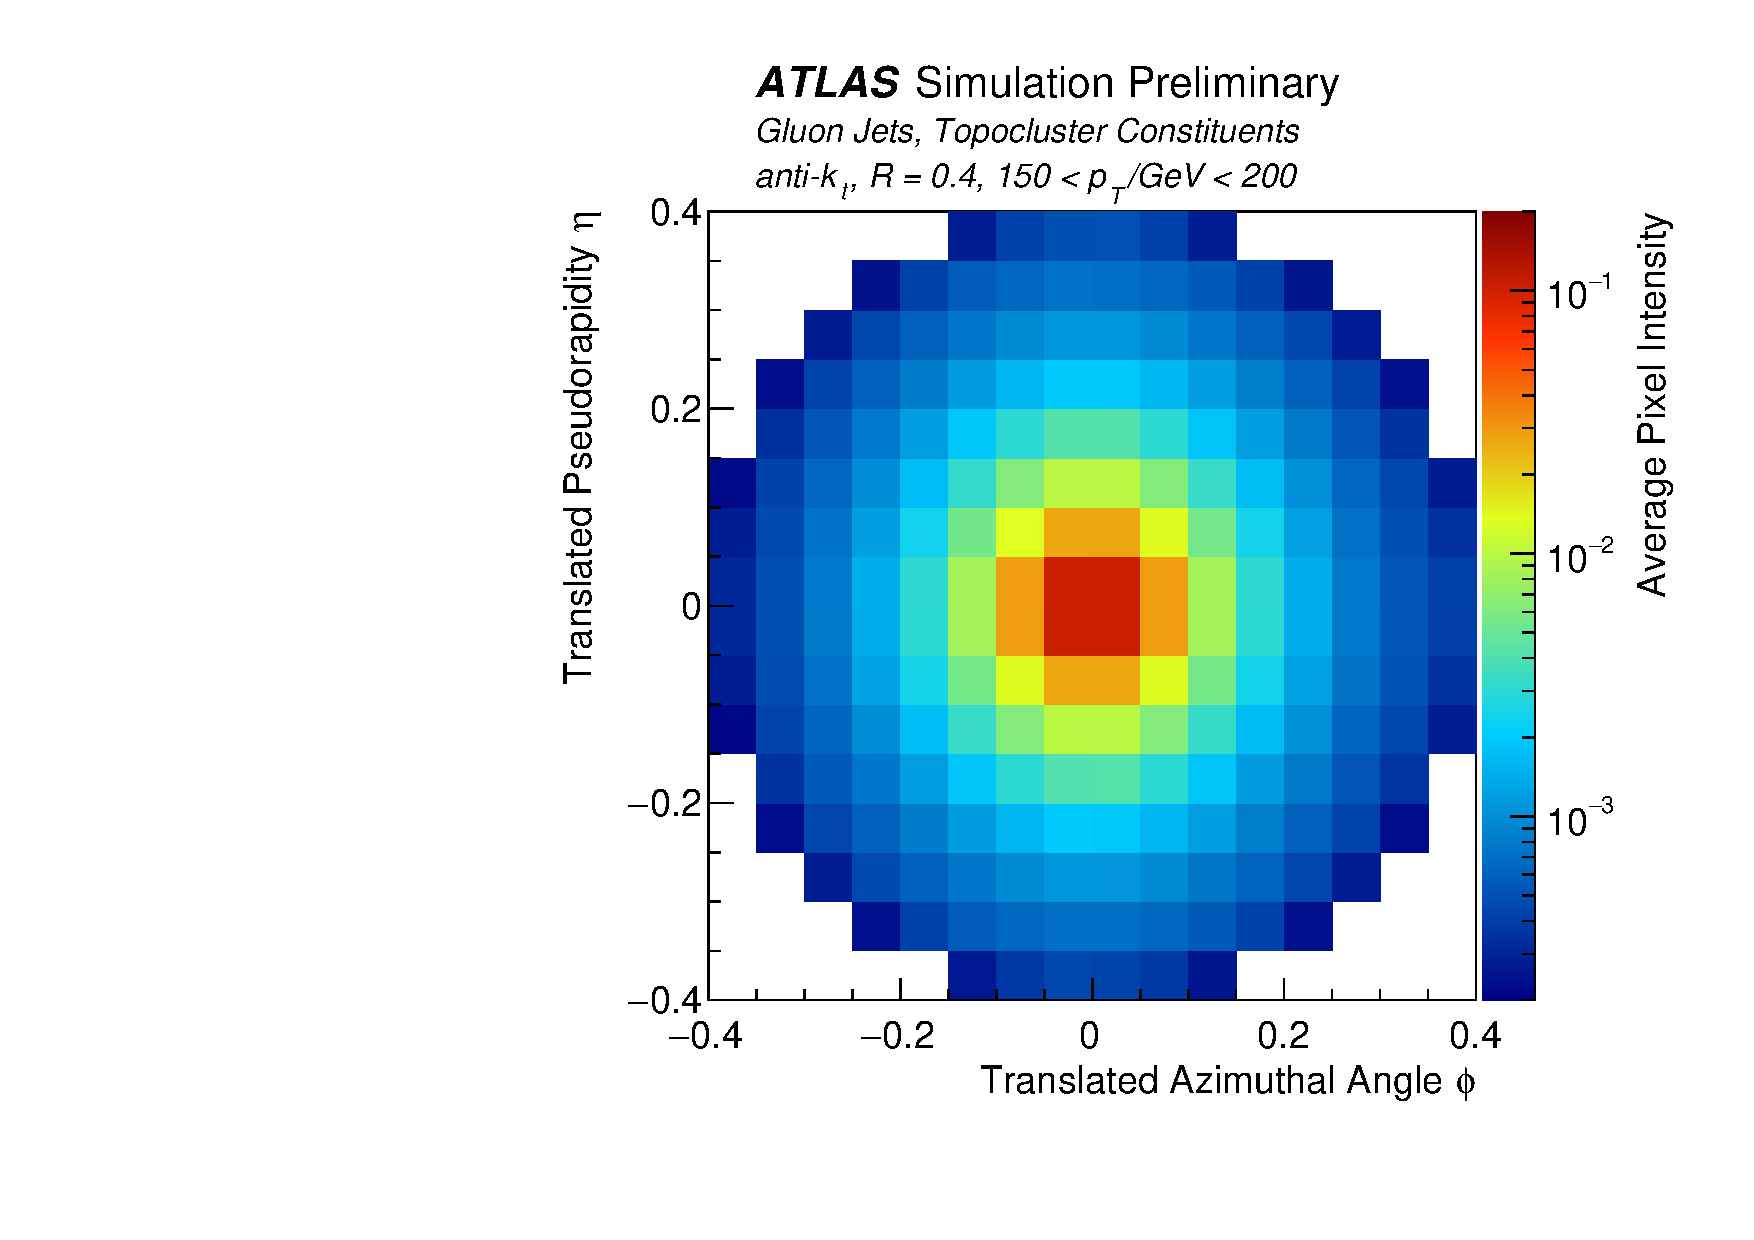
\includegraphics[width=0.31\textwidth]{figures/CNN/gluon_cluster.pdf}
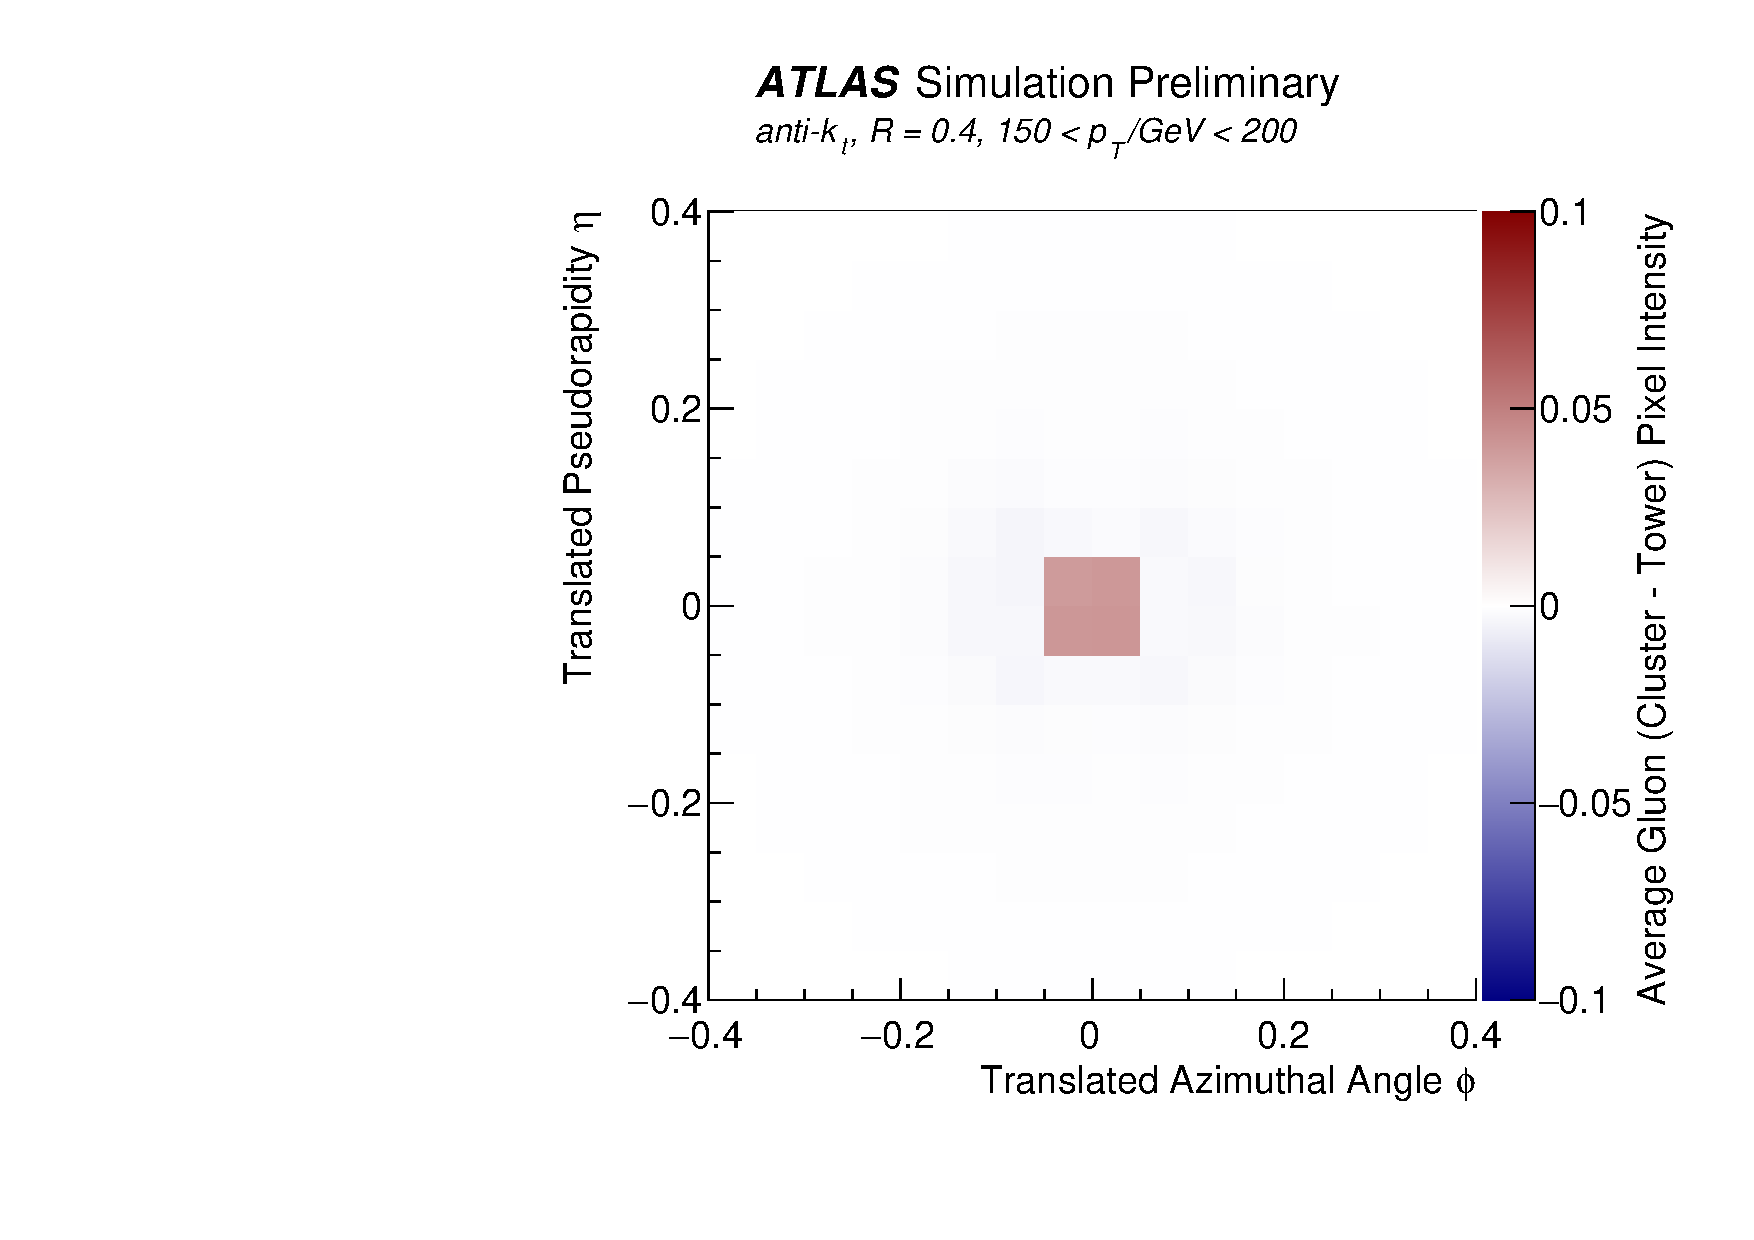
\includegraphics[width=0.31\textwidth]{figures/CNN/diff_gluon_cluster_tower.pdf}
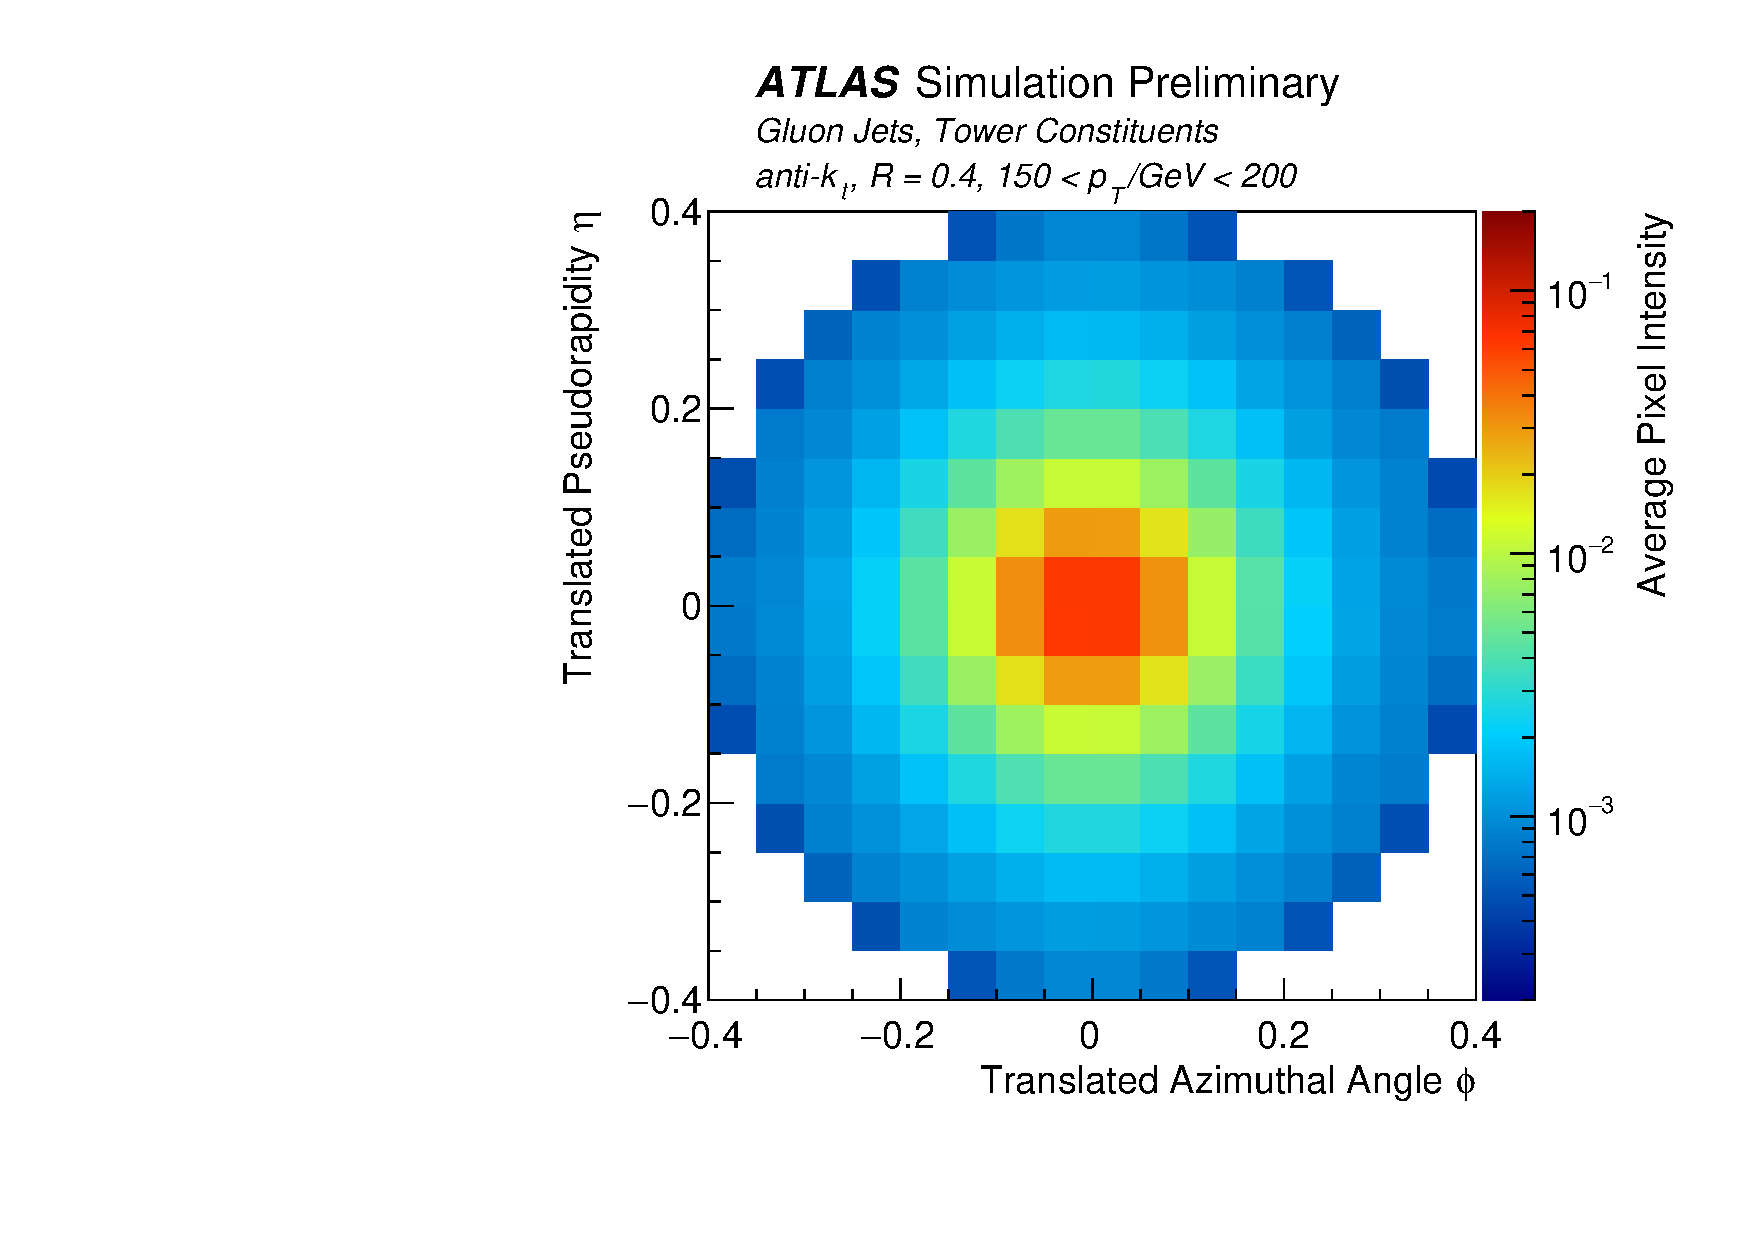
\includegraphics[width=0.31\textwidth]{figures/CNN/gluon_tower.pdf}
\caption{The four corners show the average quark (upper) and gluon (lower) jet images, from topo-clusters (left) and towers (right); the four plots on the edges show the difference between the adjacent plots, for example the top plot shows the difference between the average quark jet for topoclusters and towers. Quark-jets are more collimated than gluon ones, and topo-cluster images are more collimated than tower images.}
\label{fig:cnn-avg:clustertower}
\end{center}
\end{figure}

\clearpage



%-------------------------------------------------------------------------------
\section{CNN tagger}
\label{sec:tagger}
%-------------------------------------------------------------------------------

\subsection{Convolutional Neural Networks}
\label{sec:cnn-cnn}

Rule-based and closed-form solutions to image classification problems were the main stream techniques until the advent of deep CNNs. The AlexNet~\cite{AlexNet} in 2012's ImageNet contest suddenly improved the performance of image classifiers by a significant margin and profoundly changed the landscape of this research area.

CNNs are a class of neural networks based on convolutional layers which are modular sets of weights (convolutional filters) that operate on a small $m\times n$ patch of the input image at a time. The output of each filter is the dot-product between the weights and the pixels in the corresponding patch. Each filter is then \emph{convolved} with the input image, sliding across the entire image with a pre-determined stride and taking dot-products. It is important to note that the same set of weights for a given filter is used for the entire image otherwise the number of parameters for a CNN will explode and the network is impossible to train. The output of the operation is a new convolved image with size smaller or equal to the original image. A non-linear activation function is typically applied to each pixel of the convolved image.
Common to CNN architectures are non-covolutional down-sampling layers such as Max-pooling~\cite{MAXPOOL}.
Such layer takes non-overlapping patches of convolution outputs as input, and outputs the maximum value for each patch.
Typical CNNs are built with convolutional layers interleaved with pooling layers of different types. 

%The depth of the network is determined by the number of convolutions concatenated in the network.
%The sets of filters, the activations and the Max-pooling constitute the fundamental building block for CNNs.


\subsection{design and training of the q/g tagger}

The CNN architecture used in this study follows the example of Ref.~\cite{Komiske:2016rsd} and consists of three blocks of a convolutional layer with a
Rectified Linear Unit (ReLU) activation~\cite{RELU} and paired with a Max-pooling layer.
The last dense layer has 128 neurons with a ReLU activation taking in the flattened output from the convolutional blocks.
The output of the network is a softmax function~\cite{dlbook} of size two, 
predicting the probability for the quark jet and the gluon jet class, respectively. 
The convolutional layers consist of 128, 128 and 64 filters, with filter sizes of $5\times5$, $5\times5$ and $3\times3$, respectively.
The Max-pooling layers perform a $2\times2$ downsampling with a stride length of 2.
In order to prevent overfitting, dropout layer~\cite{Goodfellow-et-al-2016-Book} is applied to each convolution and the final fully connected layer with rate 0.3.
In addition, a L2 regularization~\cite{Goodfellow-et-al-2016-Book} with strength $10^{-8}$ is applied to all layers.  
A coarse scan of the various hyper-parameters was performed prior to settling on the architecture described above.
An illustration of the architecture used is shown in Figure~\ref{fig:networkarch}.

\begin{figure}[htpb]
\begin{center}
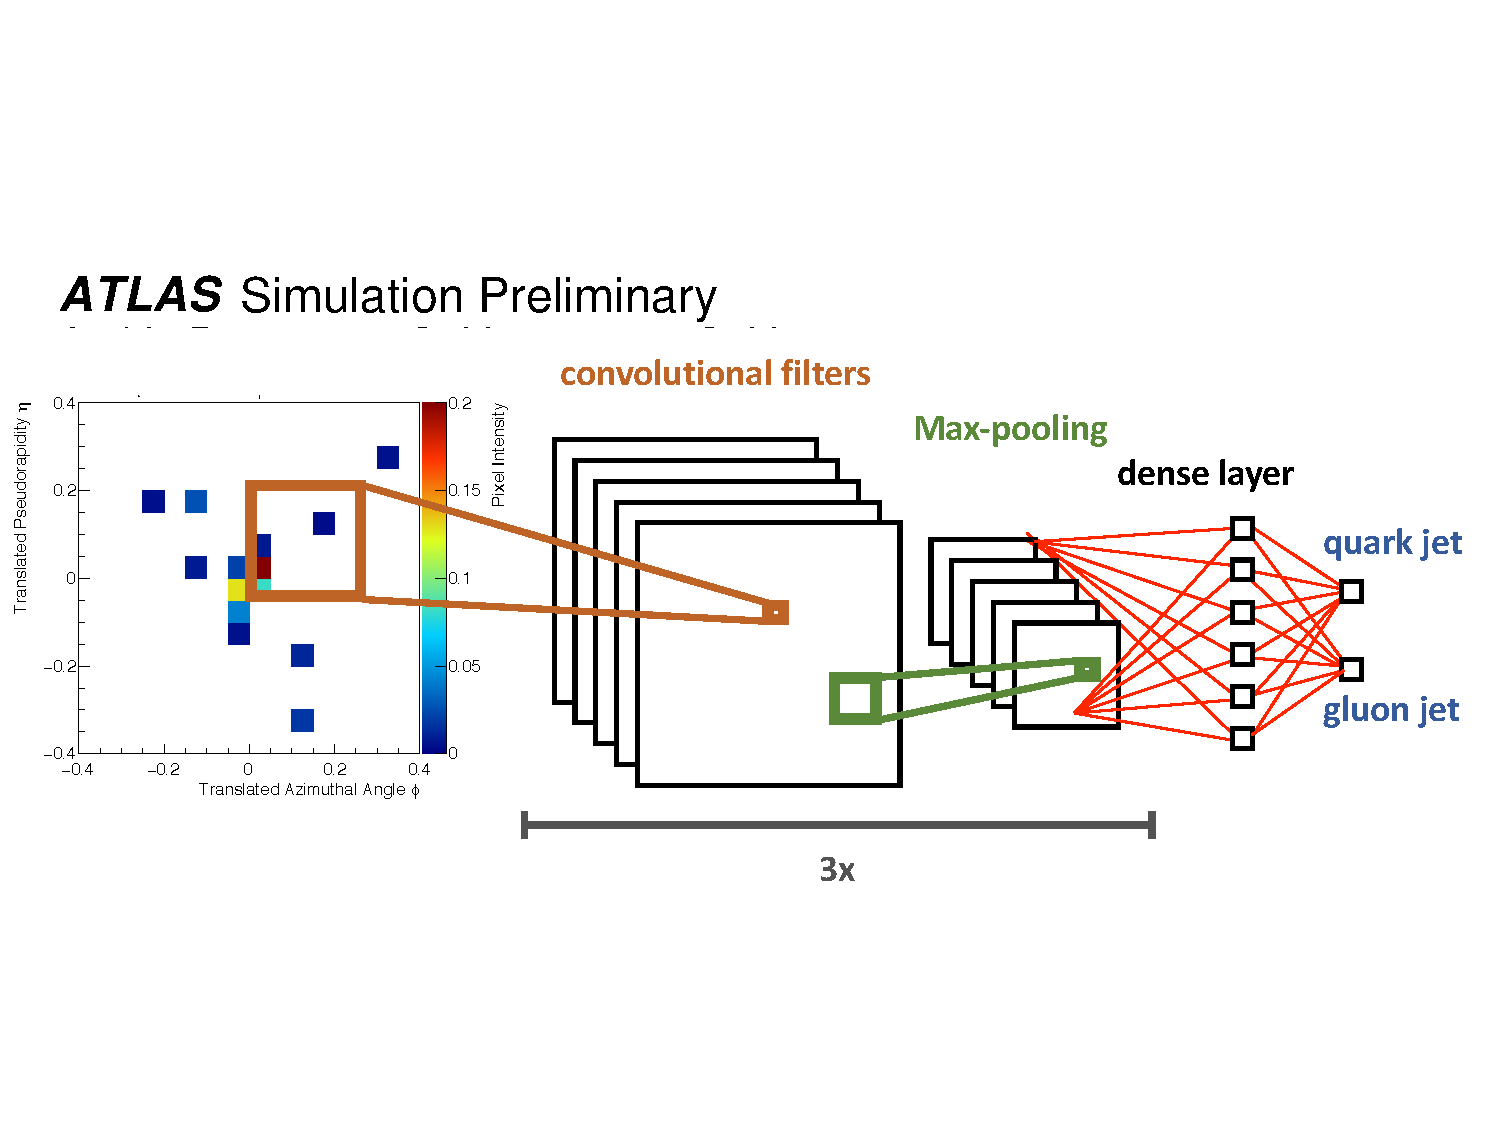
\includegraphics[width=0.8\textwidth]{figures/CNN/network.pdf}
\caption{Illustration of the deep convolutional neural network architecture.}
\label{fig:networkarch}
\end{center}
\end{figure}

Training is performed by minimizing the categorical crossentropy~\cite{Goodfellow-et-al-2016-Book}.
Minimization is performed with the Adam optimizer~\cite{DBLP:journals/corr/KingmaB14} 
as implemented in Keras~\cite{keras}
with a learning rate of 0.0001 over 50 iterations.
Training is performed using a single NVidia Tesla K80 GPU with 224000 jet images, while 56000 jet images are used for testing.
A typical training requires about 1 hour.
The network is retrained for each of the two $p_\text{T}$ ranges considered.
The output of the network corresponding to the quark jet class is used as a discriminant (\textit{CNN tagger}).


%-------------------------------------------------------------------------------
\subsection{Pileup dependence}
\label{sec:pileup}
%-------------------------------------------------------------------------------

The impact of pileup effects on the performance of the CNN tagger is evaluated 
by considering events with a different number of reconstructed primary vertices ($N_\text{PV}$).
The test sample is divided into three bins: $N_\text{PV}<13$, $13<N_\text{PV}<20$ and $N_\text{PV}>20$.  
The distributions of the pixel intensities do vary with pileup, 
but the performance of the CNN tagger is found to be robust. 
This is demonstrated by Figure~\ref{fig:pileup}. 
% shows that the efficiencies for a specific working point vary with the pileup conditions (by a similar amount as jet width), but the overall discriminating performance is not significantly degraded (ROC curve is largely invariant).

\begin{figure}[tbp]
\begin{center}
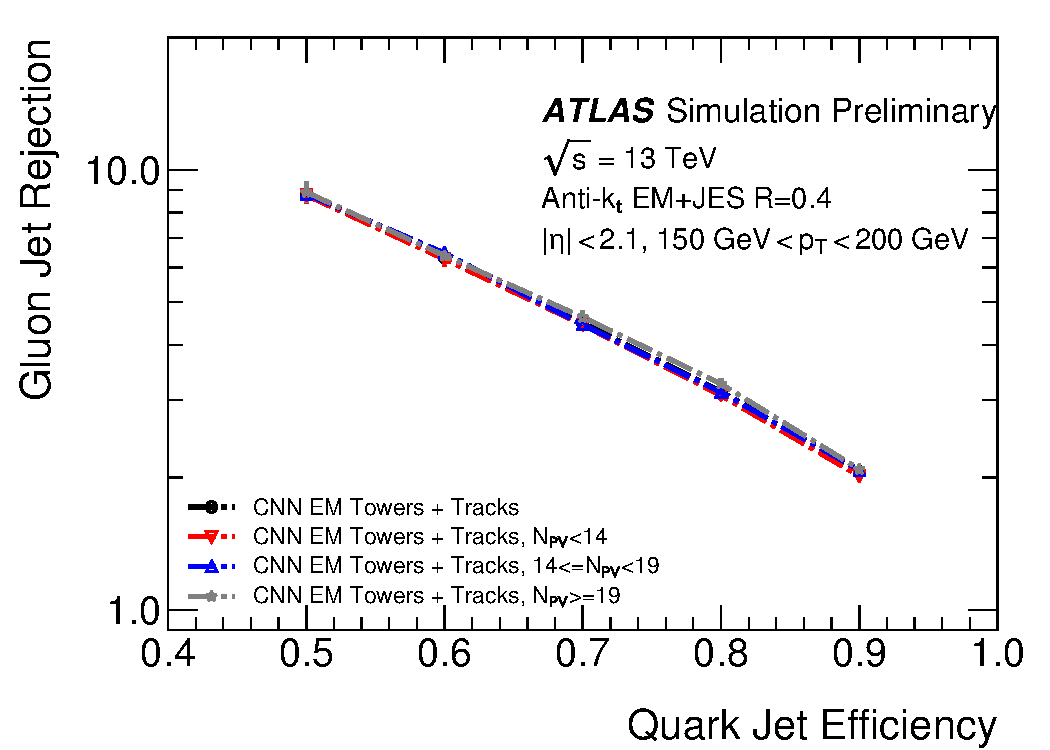
\includegraphics[width=0.5\textwidth]{figures/roc/ROC_pt150_200_NPV.pdf}
%\subfloat[][]{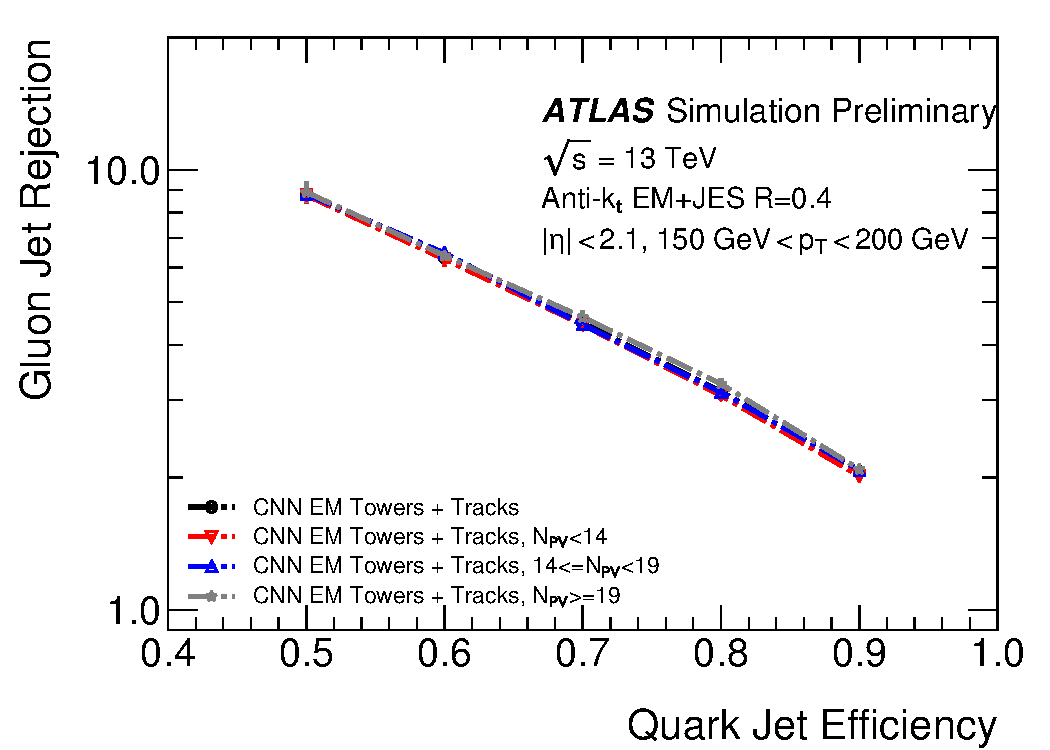
\includegraphics[width=0.5\textwidth]{figures/roc/ROC_pt150_200_NPV.pdf}\label{roc}}
%\subfloat[][]{\includegraphics[width=0.5\textwidth]{figures/roc/NPVEff.pdf}\label{eff}}
\caption{Gluon jet rejection as a function of the quark jet efficiency %\protect\subref{roc} 
evaluated at different pileup conditions, 
quantified by the number of reconstructed primary vertices ($N_\text{PV}$).}
%\protect\subref{eff} 
%Quark and gluon jet efficiency as a function of NPV for the CNN tagger.
%Jets are selected by requiring a minimum value of the CNN tagger, 
%where the threshold is chosen to give an overall 60\% quark jet efficiency.
%The efficiencies for jet width are shown for reference.}
\label{fig:pileup}
\end{center}
\end{figure}

Calorimeter-based discrimination is not only effected by in-time pileup (quantified by $N_\text{PV}$) but also by out-of-time pileup. 
Figure~\ref{fig:pileup2} compares the tagger performance in two different regimes of the average number of collisions per bunch crossing ($\mu$) regimes corresponding to the out-of-time pileup representative of LHC Run 2 conditions.

\begin{figure}[tbp]
\begin{center}
\subfloat[][]{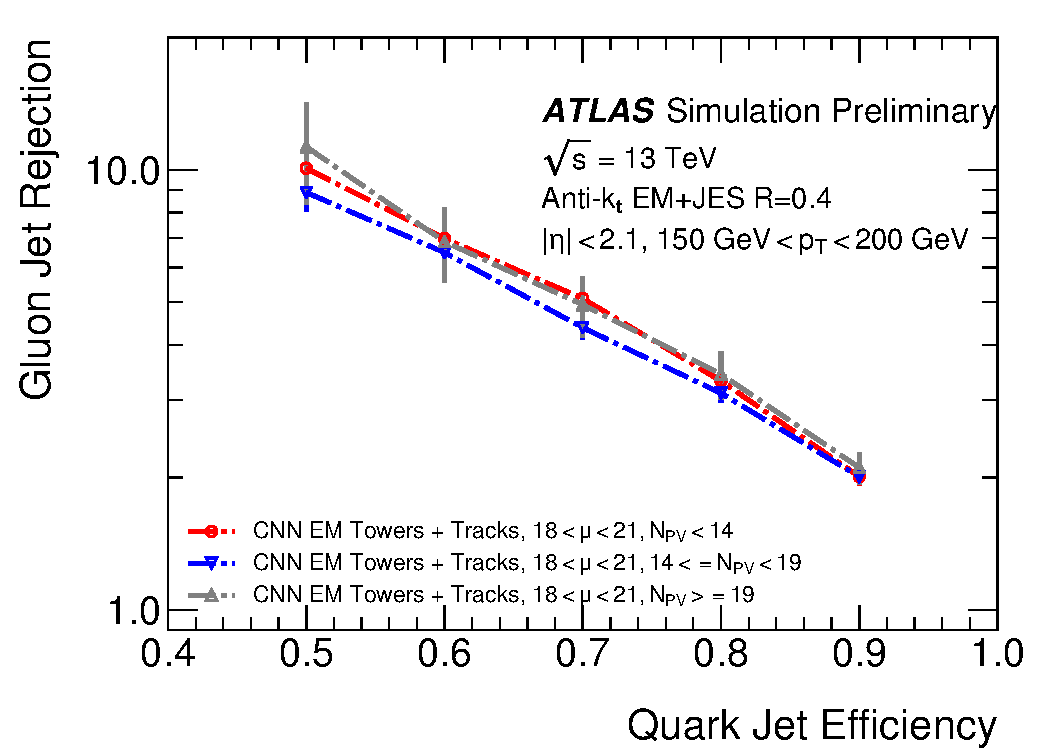
\includegraphics[width=0.5\textwidth]{figures/roc/ROC_pt150_200_mu18_21.pdf}\label{roc1}}
\subfloat[][]{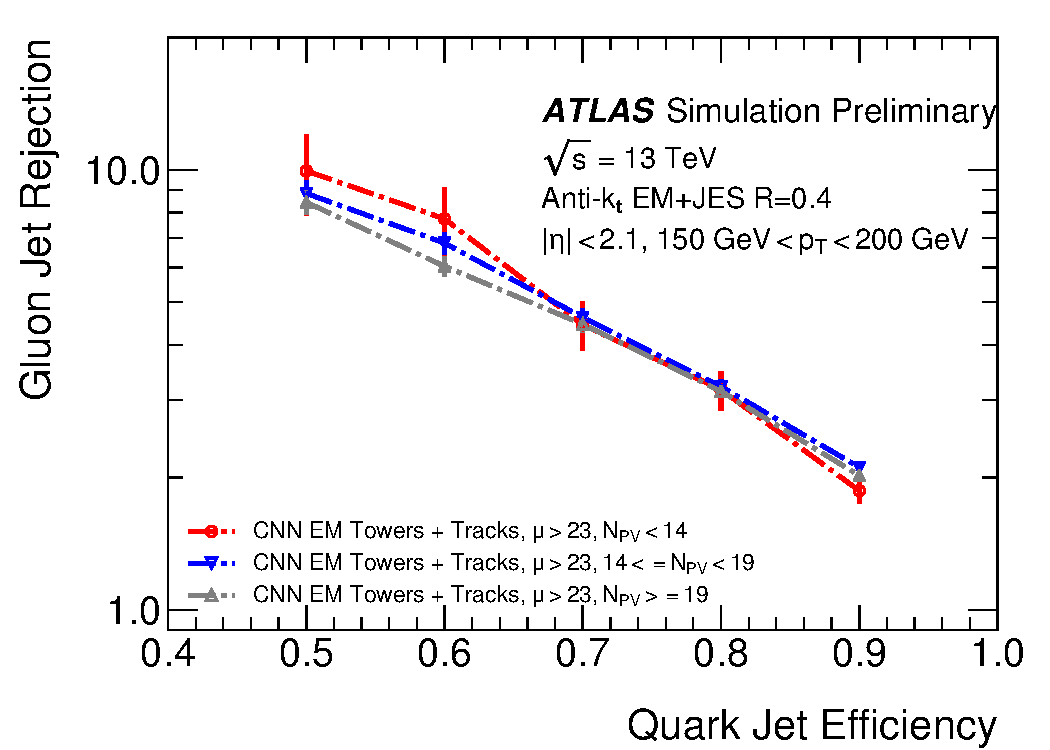
\includegraphics[width=0.5\textwidth]{figures/roc/ROC_pt150_200_mu23.pdf}\label{roc2}}
\caption{Gluon jet rejection as a function of the quark jet efficiency 
evaluated at different levels of $N_\text{PV}$ for \protect\subref{roc1} $18<\mu<23$ and \protect\subref{roc2}  $\mu > 23$.
The two $\mu$ bins where chosen to have roughly the same number of events.}
\label{fig:pileup2}
\end{center}
\end{figure}


%-------------------------------------------------------------------------------
\subsection{Fragmentation modeling}
\label{sec:frag}
%-------------------------------------------------------------------------------

Quark versus gluon tagging is sensitive to the detailed modeling of perturbative and non-perturbative effects involved with fragmentation.  
We compare images and image classification performance with two very different fragmentation models.  
Figure~\ref{fig:avg:pythiasherpa} shows the average image (differences) between quark and gluon jets simulated with 
\textsc{Pythia} 8 and with \textsc{Herwig++}.  
The radiation pattern inside gluon jets is similar between the two models, whereas there are larger differences for quark jets.  
In particular, quark and gluon jets are more different according to \textsc{Pythia} 8 relative to \textsc{Herwig++}.  
This is observed with the CNN in Fig.~\ref{fig:pythiasherpa}.  
As gluon jets in \textsc{Herwig++} are more similar to quark jets than in \textsc{Pythia} 8, 
any observable (including the CNN tagger output) tends to have less discrimination power when tested in \textsc{Herwig++}.
The training sample determines the nature of the observable the CNN tagger learns. 
By comparing the CNN tagger trained on \textsc{Pythia} 8 events with the one trained on \textsc{Herwig++} events
using the same test sample (\textsc{Pythia} 8),
we see a smaller discrepancy, indicating that the learned feature is not strongly sensitive 
to the difference between \textsc{Pythia} 8 and \textsc{Herwig++}.
\textsc{Pythia} 8 and \textsc{Sherpa} produce relatively similar images and so unsurprisingly, 
the CNN performance is similar when trained/tested on either of these generators.  
As also noted by Ref.~\cite{Barnard:2016qma}, when generators produce different images, 
the CNN returns a different performance when training and testing with images from various simulators.  
However, if the same network is used for testing and only the training sample is varied, 
the gap in performance is mostly removed (see also~\cite{Komiske:2016rsd}).  
One explanation is that the network is learning robust features for quark versus gluon tagging, 
but the degree to which the features are expressed in the radiation patterns varies between generators.

%As alternative to the baseline \textsc{Pythia} 8 sample described in Section~\ref{sec:images},  we consider a dijet sample generated with \textsc{SHERPA} (v2.2.0)~\cite{Gleisberg:2008ta} and the CT10 PDF set. Interestingly, the models themselves result in similar images, shown in Figure~\ref{fig:avg:truthtrack}, and not surprisingly, Figure~\ref{fig:pythiasherpa} shows that the tagger performance is also similar.

\begin{figure}[tbp]
\begin{center}
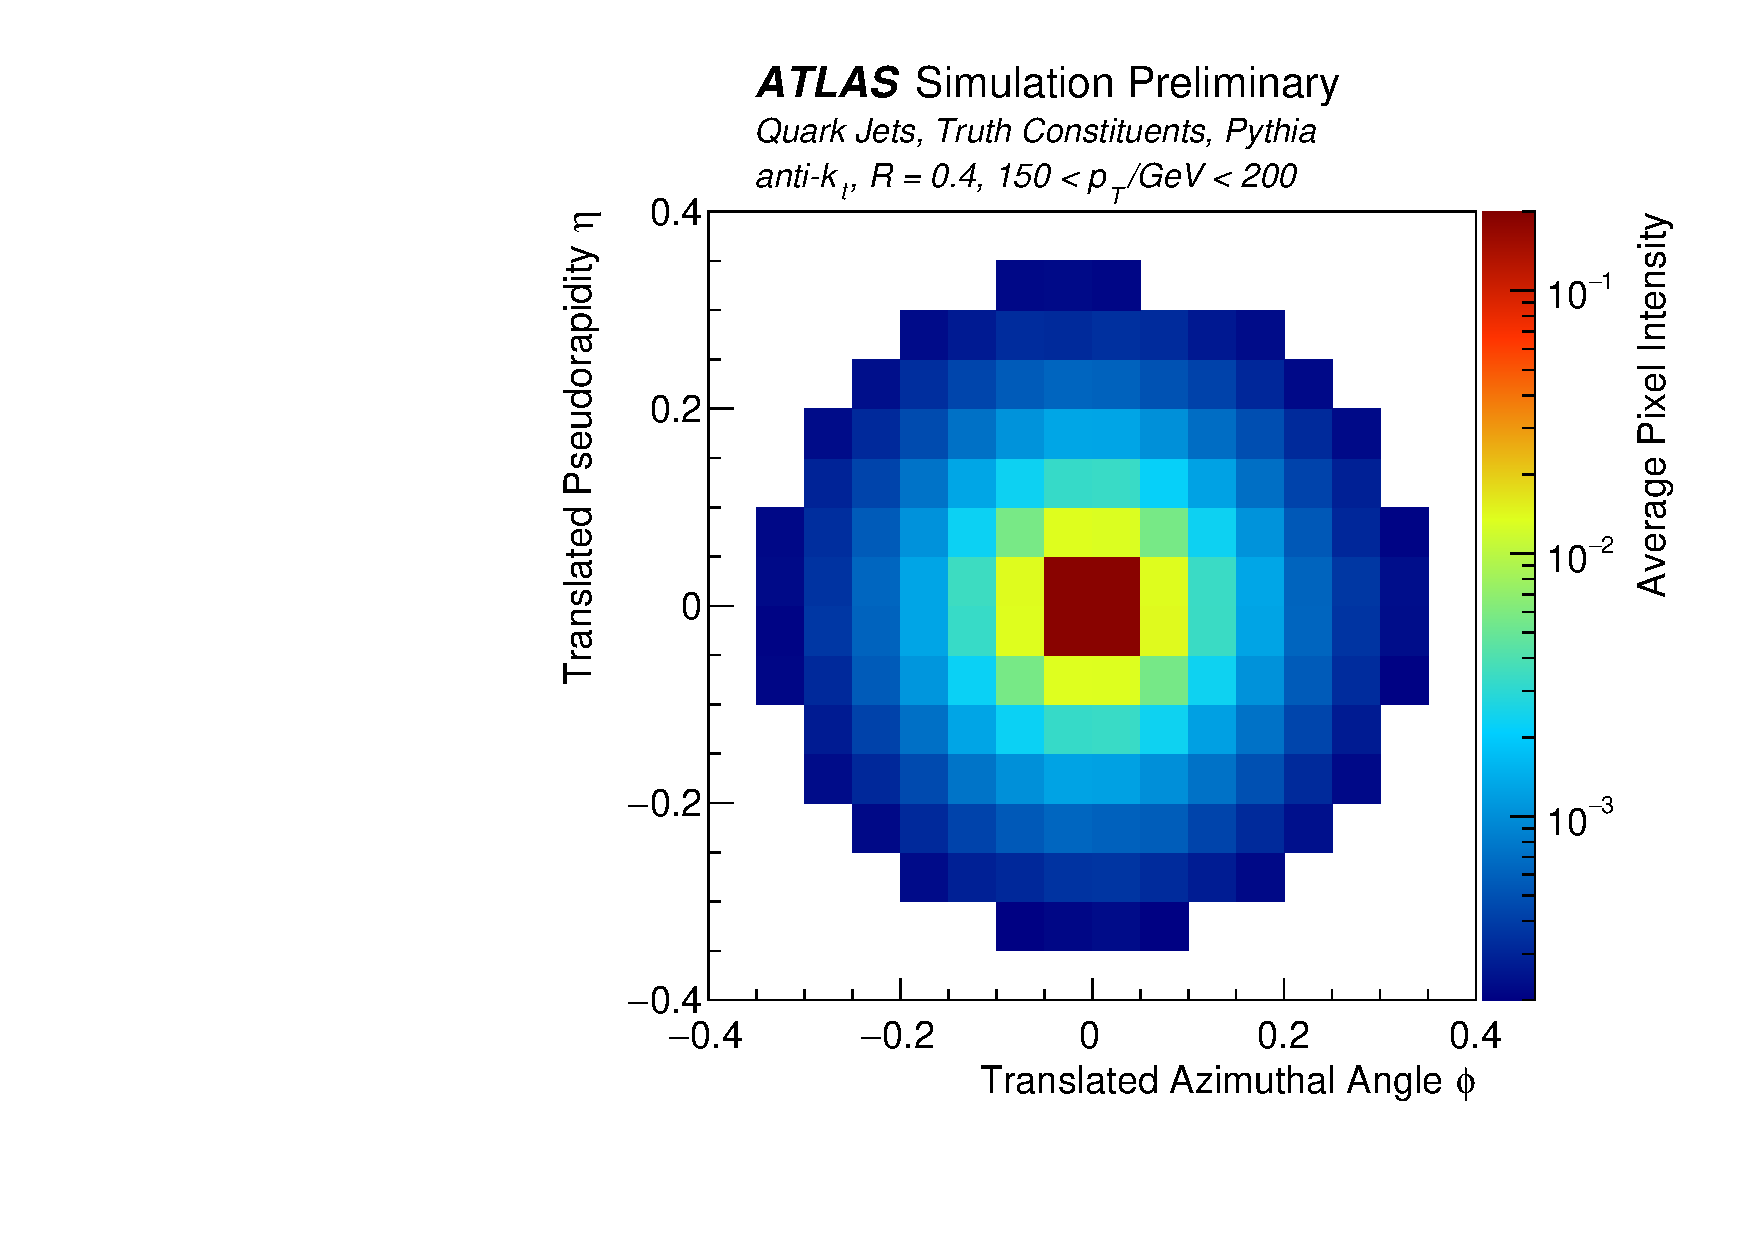
\includegraphics[width=0.33\textwidth]{figures/pythiasherpa/quark_truth_pythia.pdf}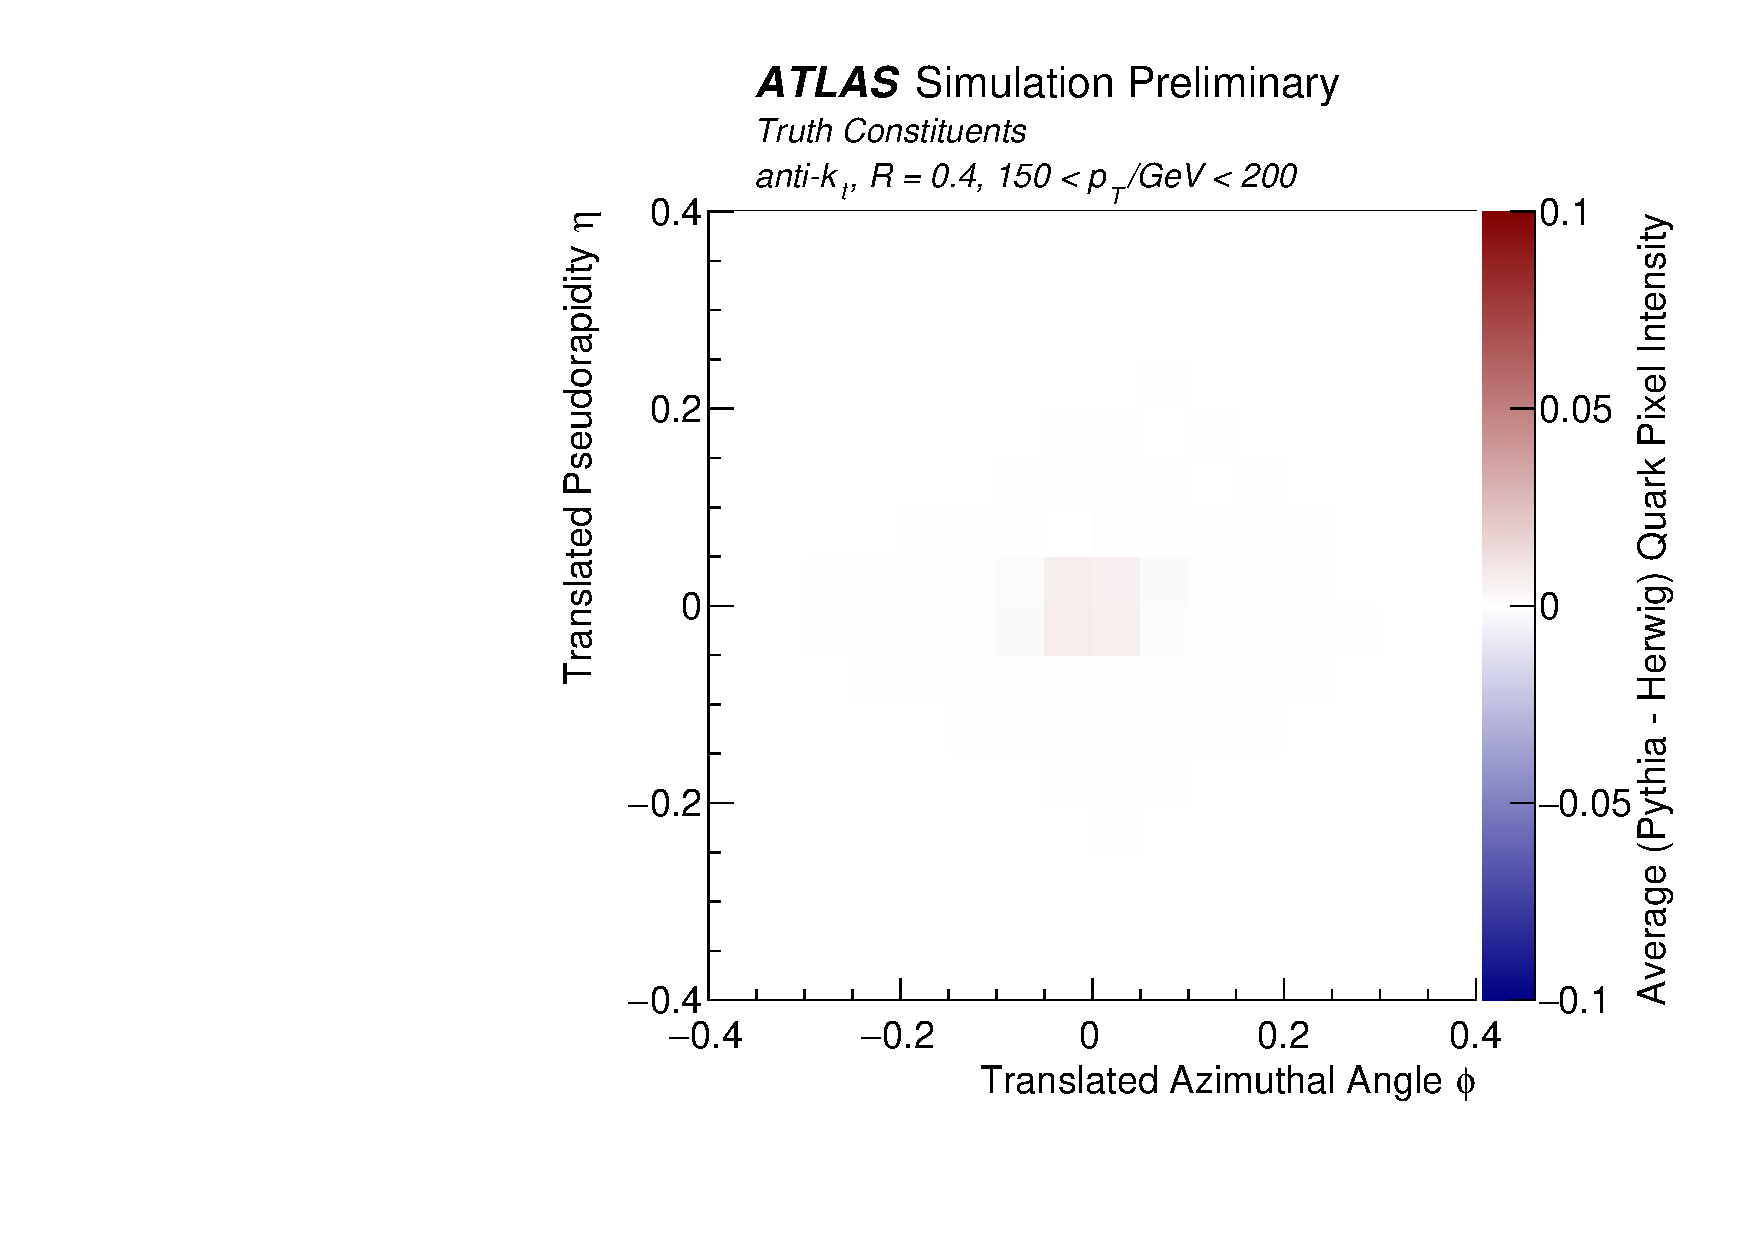
\includegraphics[width=0.33\textwidth]{figures/pythiasherpa/diff_truthq_pythiaherwig.pdf}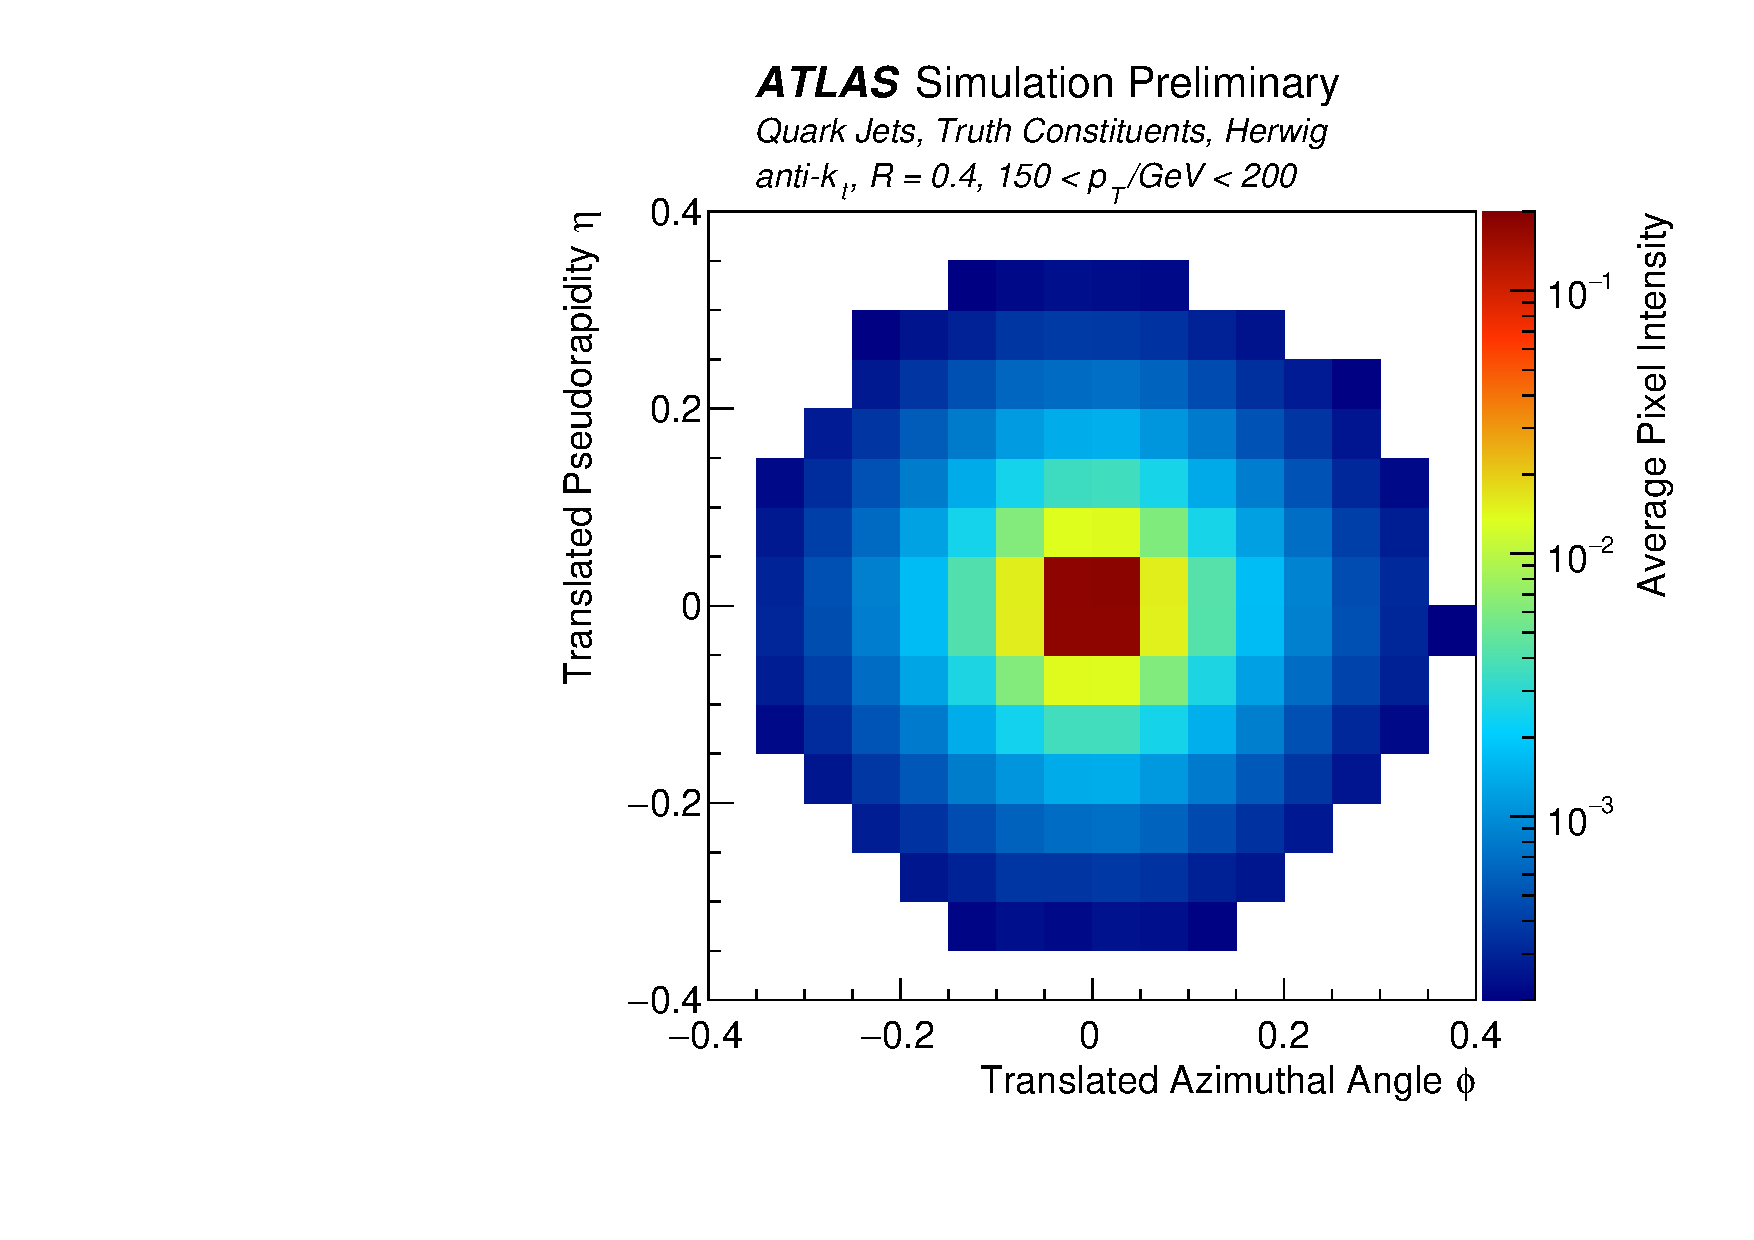
\includegraphics[width=0.33\textwidth]{figures/pythiasherpa/quark_truth_herwig.pdf}\\
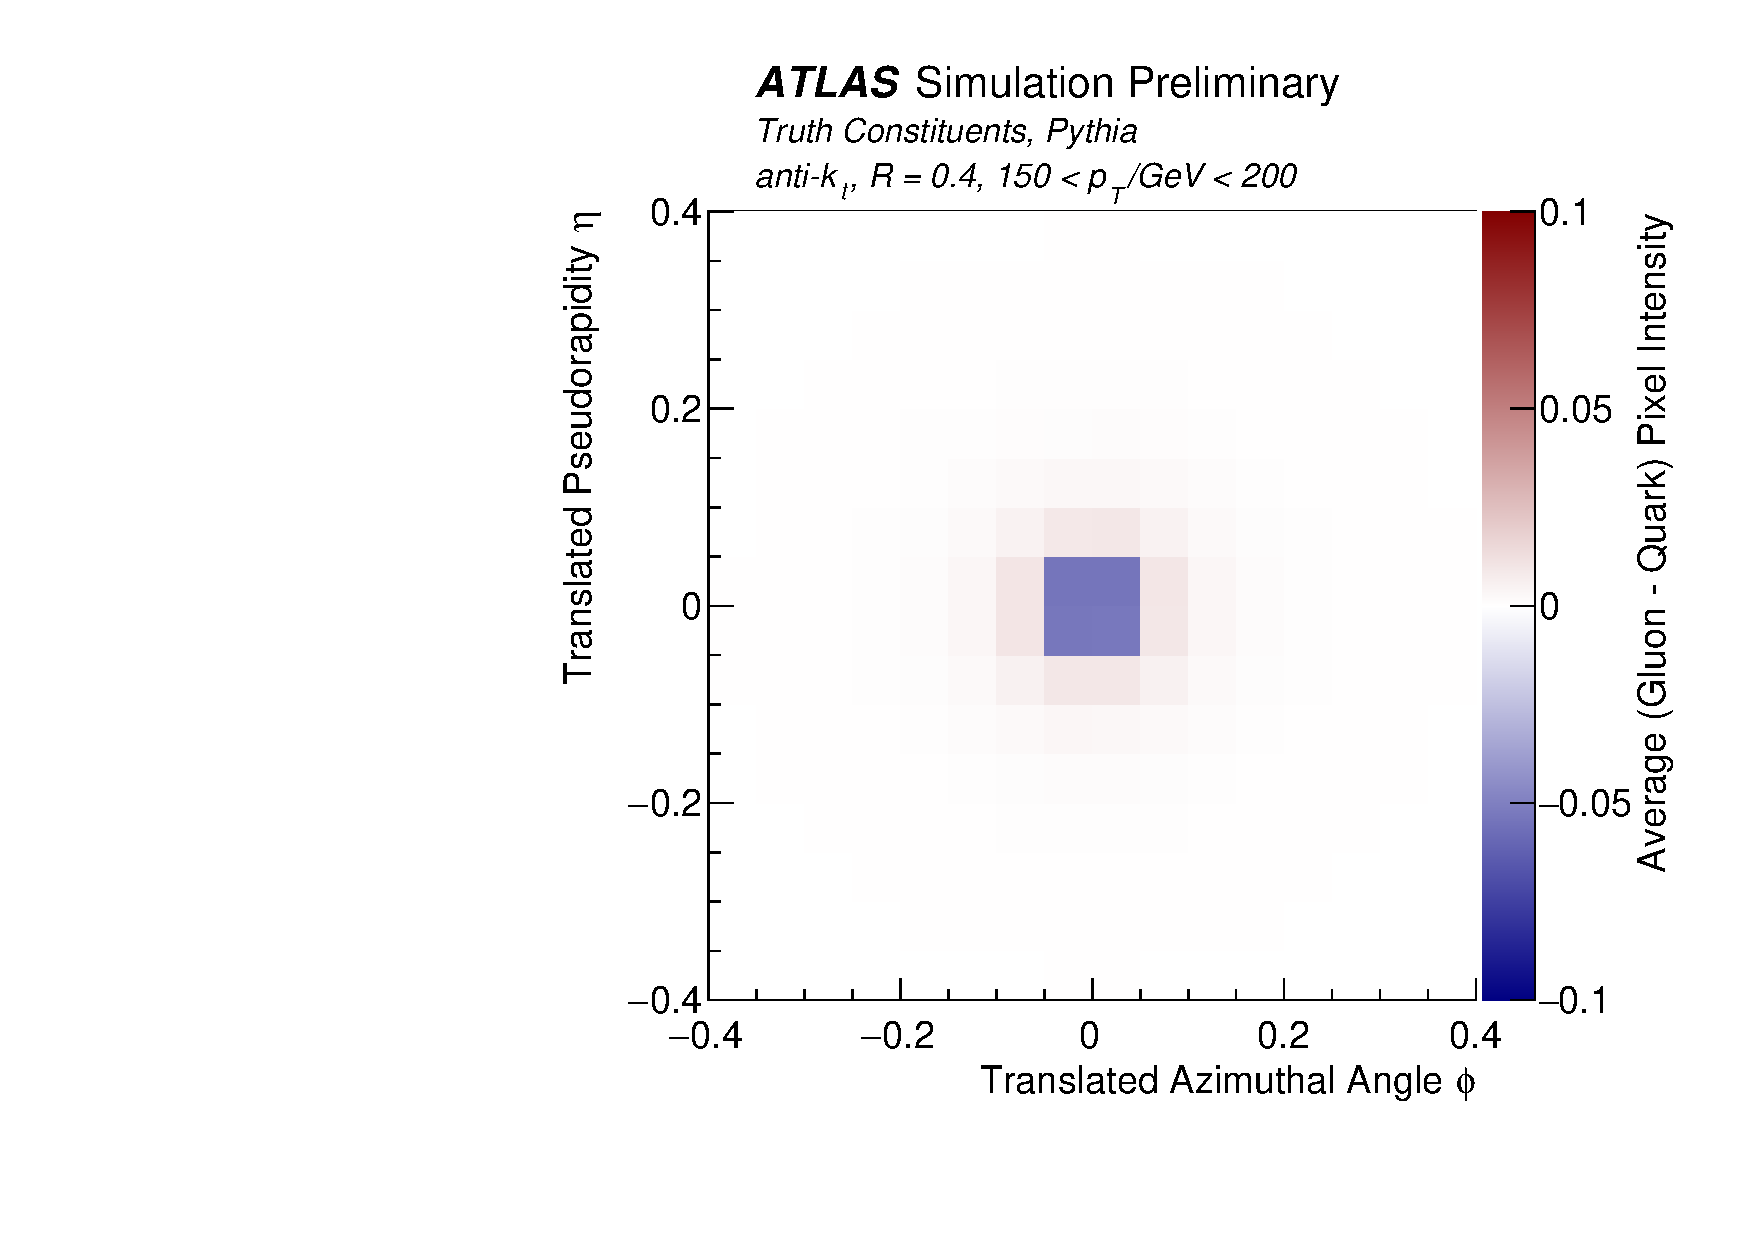
\includegraphics[width=0.33\textwidth]{figures/pythiasherpa/diff_truth_pythia.pdf}\hspace{54mm}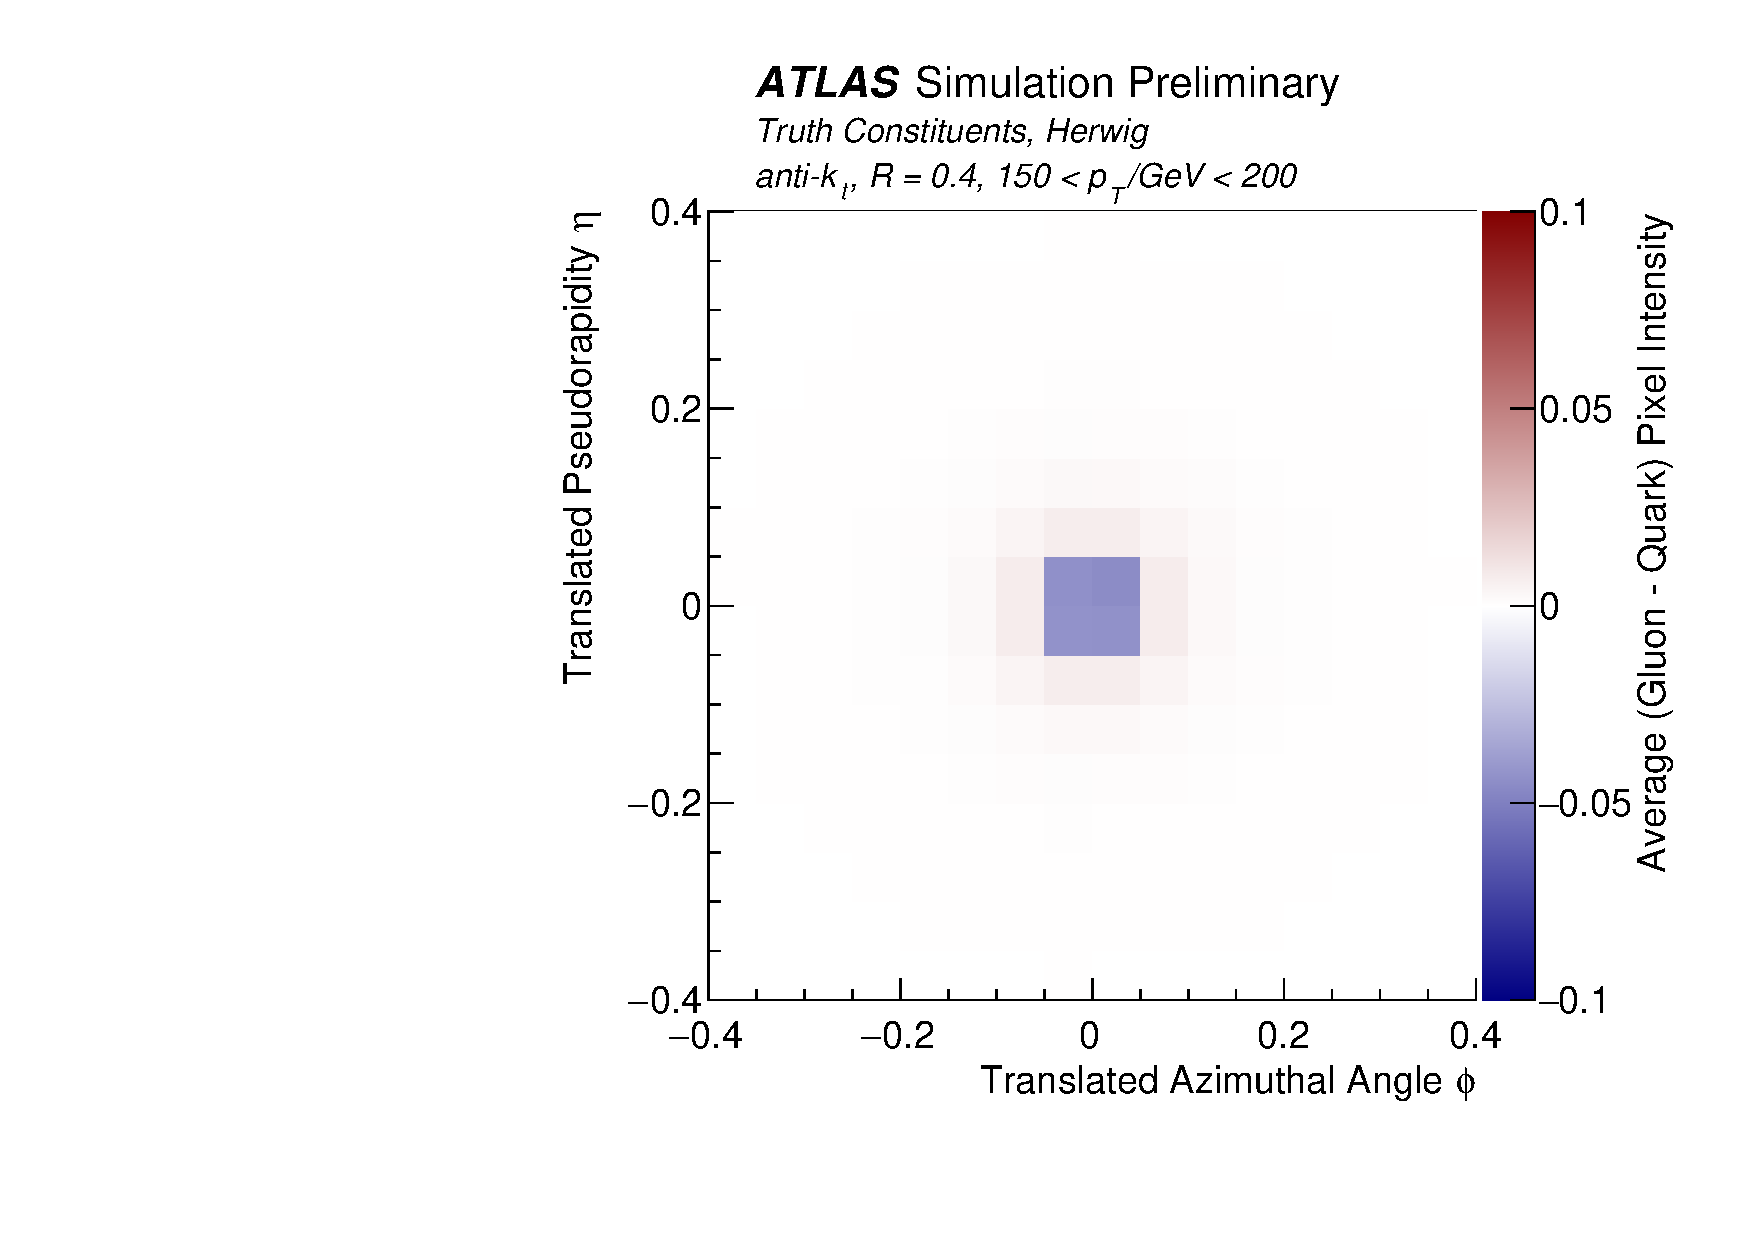
\includegraphics[width=0.33\textwidth]{figures/pythiasherpa/diff_truth_herwig.pdf}\\
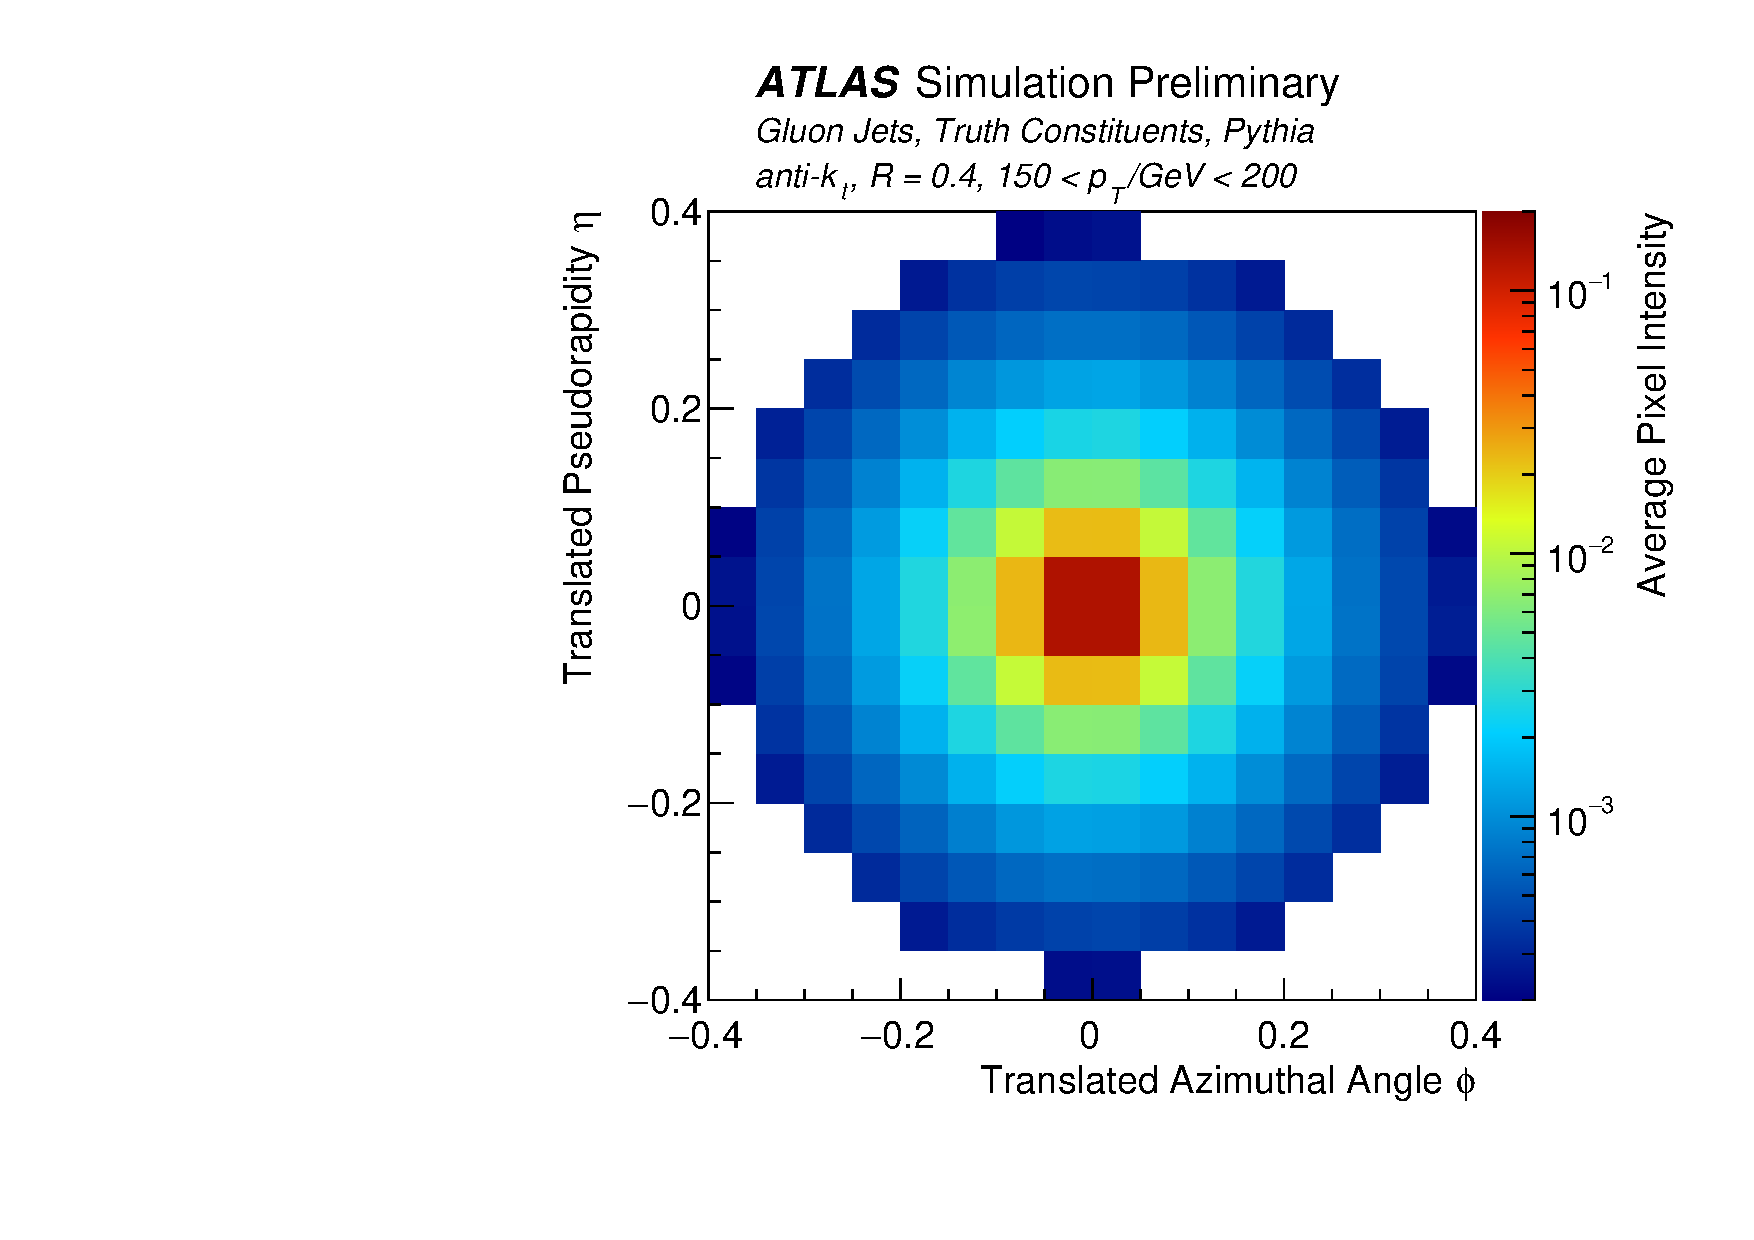
\includegraphics[width=0.33\textwidth]{figures/pythiasherpa/gluon_truth_pythia.pdf}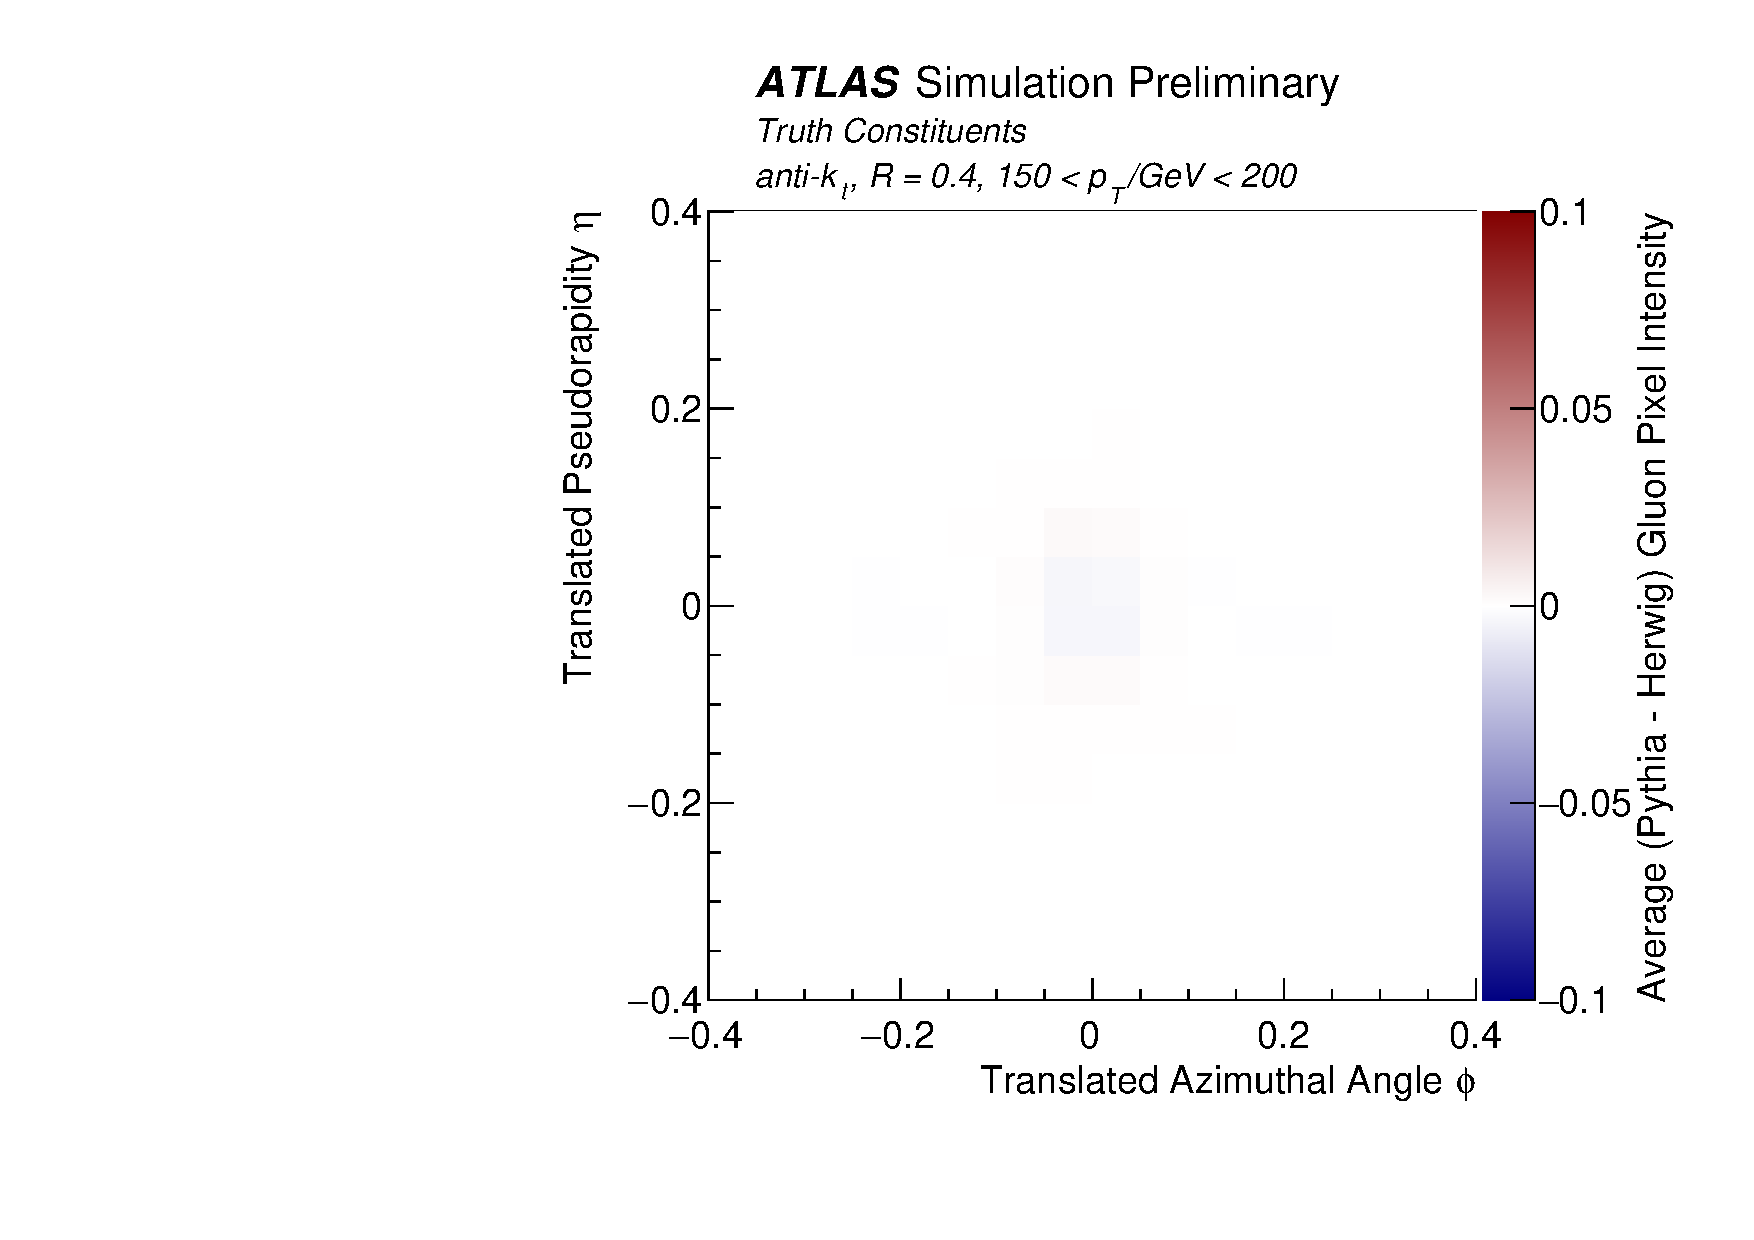
\includegraphics[width=0.33\textwidth]{figures/pythiasherpa/diff_truthg_pythiaherwig.pdf}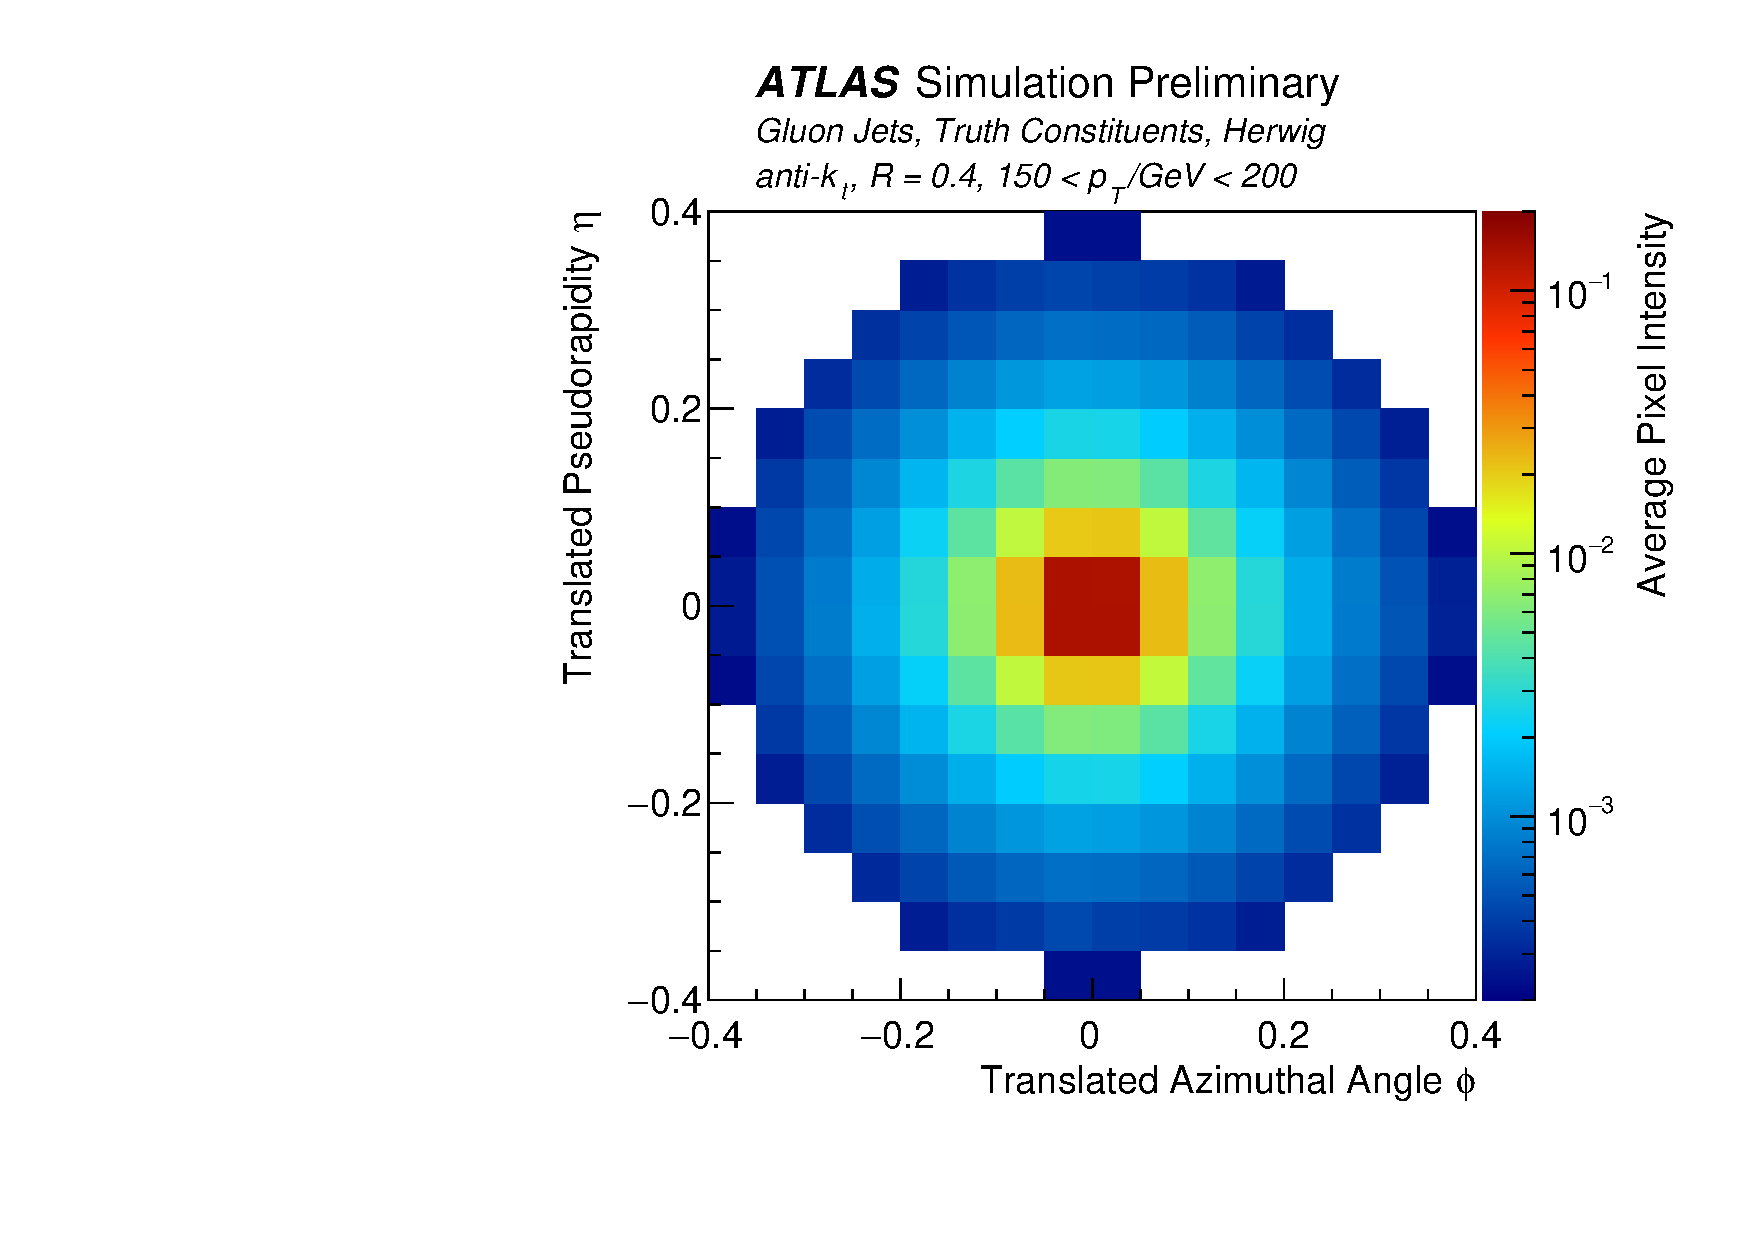
\includegraphics[width=0.33\textwidth]{figures/pythiasherpa/gluon_truth_herwig.pdf}
\caption{
The four corners show the average quark (top) and gluon (bottom) jet images, for jets generated with \textsc{Pythia} (left) and
and \textsc{Herwig} (right); the four plots on the edges show the difference between the adjacent plots,
for example the top plot shows the difference between the average quark jet in \textsc{Pythia} and
and \textsc{Herwig}.}
\label{fig:avg:pythiasherpa}
\end{center}
\end{figure}


\begin{figure}[h!]
\begin{center}
\subfloat[][]{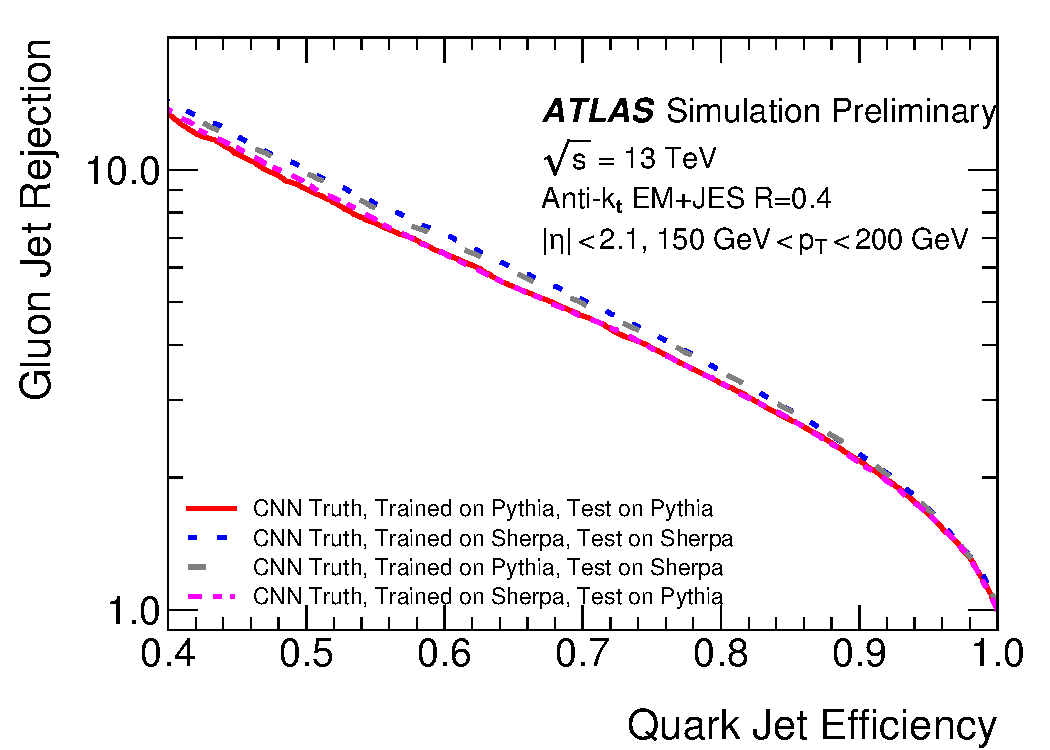
\includegraphics[width=0.5\textwidth]{figures/roc/ROC_pt150_200_gen_pythia_sherpa.pdf}\label{pythiasherpa}} 
\subfloat[][]{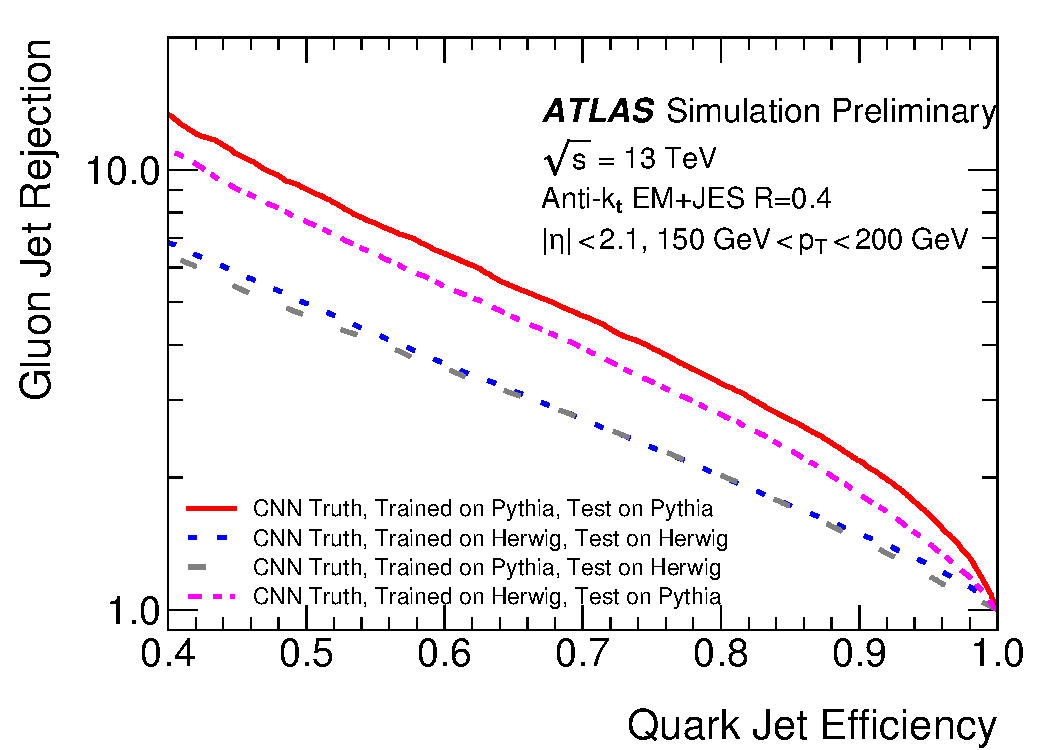
\includegraphics[width=0.5\textwidth]{figures/roc/ROC_pt150_200_gen_pythia_herwig.pdf}\label{pythiaherwig}} 
\caption{Gluon jet rejection as a function of the quark jet efficiency comparing \textsc{Pythia} to \protect\subref{pythiasherpa} \textsc{Sherpa}
and \protect\subref{pythiaherwig} \textsc{Herwig} for jets with $150<\pt<200~\GeV$.}
\label{fig:pythiasherpa}
\end{center}
\end{figure}




%-------------------------------------------------------------------------------
\subsection{Visualizing learned information}
\label{sec:learningaboutlearning}
%-------------------------------------------------------------------------------

Interpretability is always a concern for applying deep neural networks
with complicated structures. It is essential for us to make sure that the
CNN taggers we build yield results which at least conform to our physics intuition.
The first cross check performed following the strategy in Ref.~\cite{deOliveira:2015xxd} calculates
the Pearson Correlation Coefficient of the per pixel intensity with the CNN output score.
As shown in Figure ~\ref{fig:correlation}, the pixel intensity of the core of the image is strongly
 correlated with the output, meaning that the more heavily centered the image is the more likely
the jet is a quark. The intensity of the outer peripheral pixels are anti-correlated with
the CNN output, consistent with the fact that gluon jets tend to have a broader radiation pattern. 

The convolutional filters of CNN can be viewed as capturing features which are distinct to different
class of images. Investigation of these filters will provide useful information of what the CNN regard as
important difference between quarks and gluons. Formally, we examine the difference of applying the
convolutional filters to the average image of quarks($I_q$) and gluons($I_g$), i.e. computing $I_q * w_i - I_g * w_i$,
where $*$ is the convolution operator and $w_i$ denotes the individual filters. The visualizations for the
filters in the first convolutional layer are shown in Figure~\ref{fig:filters}.
Many such difference images are rotational copies of each other as the CNN is able to capture the rotational
invariance. Some of these images are similar to the correlation plot in Figure ~\ref{fig:correlation} suggesting
the radial image difference is one important feature while others are more complex. 

\begin{figure}[htbp]
\begin{center}
\subfloat[][]{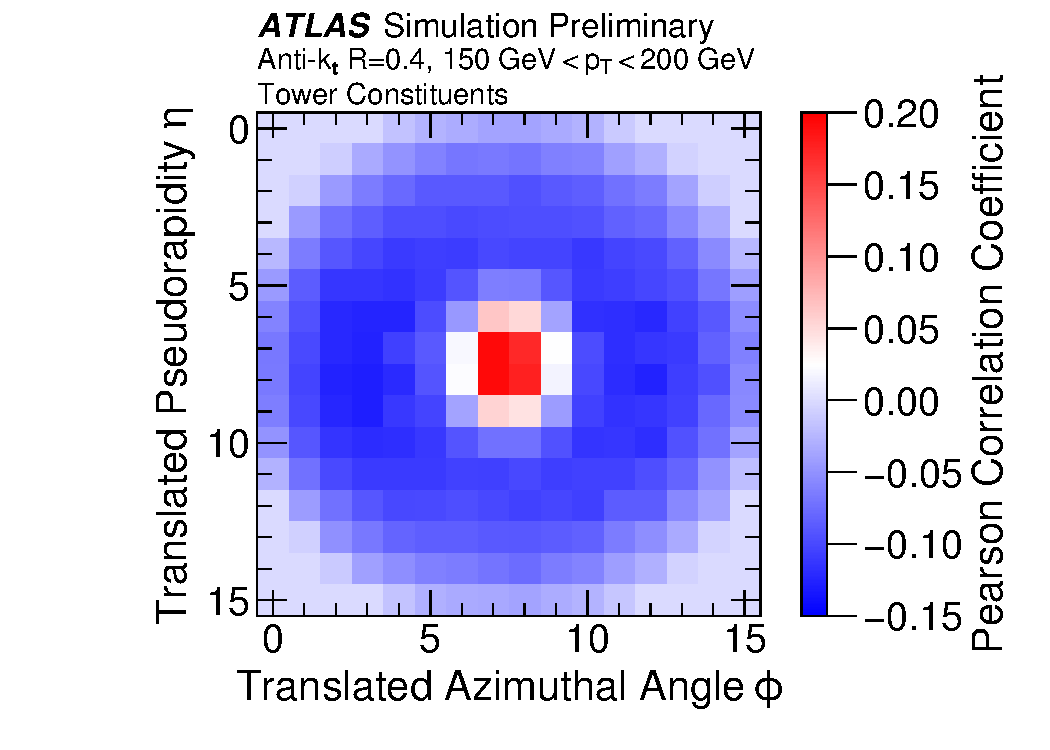
\includegraphics[width=0.7\textwidth]{figures/CNN/corr_tower150200.pdf}}
\caption{
Per-pixel linear correlation with CNN tagger output.
}
\label{fig:correlation}
\end{center}
\end{figure}

\begin{figure}[htbp]
\begin{center}
\subfloat[][]{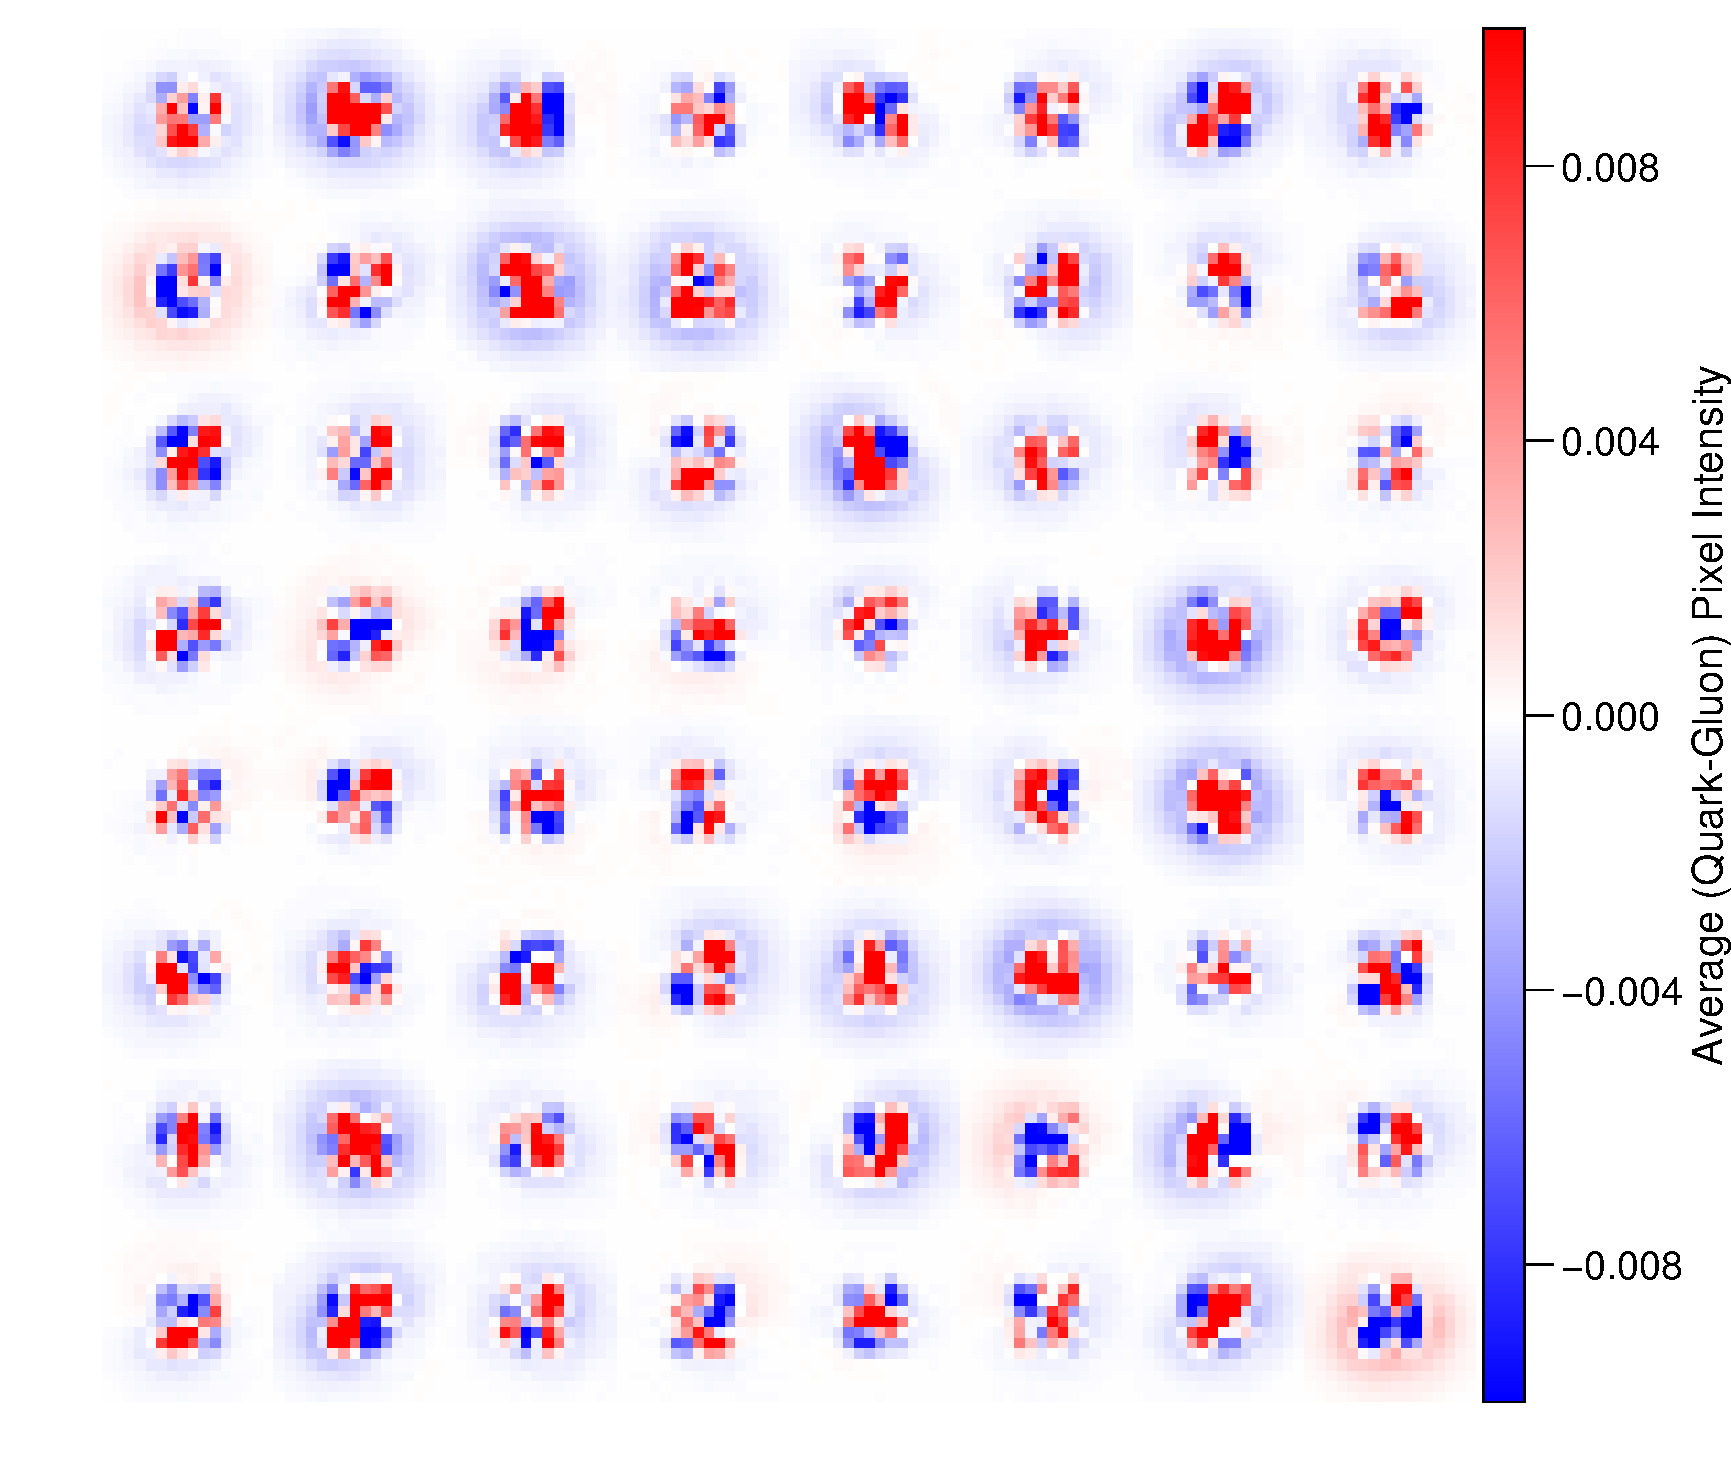
\includegraphics[width=0.9\textwidth]{figures/CNN/convimage_diff.pdf}}
\caption{
Average convolved filter differences for jet images (same color scheme as left plot; red is more quark-like). 
The filters of the first convolutional layer are considered.}
\label{fig:filters}
\end{center}
\end{figure}


%-------------------------------------------------------------------------------
%\section{Topology dependence}
%\label{sec:topo}
%-------------------------------------------------------------------------------

%\input{tex/topo.tex}


% All figures and tables should appear before the summary and conclusion.
% The package placeins provides the macro \FloatBarrier to achieve this.
 \FloatBarrier


%-------------------------------------------------------------------------------
\section{Conclusion}
\label{sec:conclusion}
%-------------------------------------------------------------------------------

This note presents the first full simulation study of deep learning with jet images.  Convolutional neural networks are used to distinguish images of the radiation pattern inside quark jets from the pattern inside gluon jets.  Across a wide range of quark jet efficiencies, the CNN tagger achieves a gluon jet rejection that is comparable to or better than the performance of classical quark versus gluon  tagging observables jet width and track multiplicity.  Furthermore, the origin of the CNN performance is investigated, including a variation of experimental conditions.  The image-based approach described in this note is a promising avenue for future research to confront a variety of tagging challenges.

%-------------------------------------------------------------------------------
%\section*{Acknowledgements}
%-------------------------------------------------------------------------------

%% Acknowledgements for papers with collision data
% Version 14-Feb-2018

% Standard acknowledgements start here
%----------------------------------------------
We thank CERN for the very successful operation of the LHC, as well as the
support staff from our institutions without whom ATLAS could not be
operated efficiently.

We acknowledge the support of ANPCyT, Argentina; YerPhI, Armenia; ARC, Australia; BMWFW and FWF, Austria; ANAS, Azerbaijan; SSTC, Belarus; CNPq and FAPESP, Brazil; NSERC, NRC and CFI, Canada; CERN; CONICYT, Chile; CAS, MOST and NSFC, China; COLCIENCIAS, Colombia; MSMT CR, MPO CR and VSC CR, Czech Republic; DNRF and DNSRC, Denmark; IN2P3-CNRS, CEA-DRF/IRFU, France; SRNSFG, Georgia; BMBF, HGF, and MPG, Germany; GSRT, Greece; RGC, Hong Kong SAR, China; ISF, I-CORE and Benoziyo Center, Israel; INFN, Italy; MEXT and JSPS, Japan; CNRST, Morocco; NWO, Netherlands; RCN, Norway; MNiSW and NCN, Poland; FCT, Portugal; MNE/IFA, Romania; MES of Russia and NRC KI, Russian Federation; JINR; MESTD, Serbia; MSSR, Slovakia; ARRS and MIZ\v{S}, Slovenia; DST/NRF, South Africa; MINECO, Spain; SRC and Wallenberg Foundation, Sweden; SERI, SNSF and Cantons of Bern and Geneva, Switzerland; MOST, Taiwan; TAEK, Turkey; STFC, United Kingdom; DOE and NSF, United States of America. In addition, individual groups and members have received support from BCKDF, the Canada Council, CANARIE, CRC, Compute Canada, FQRNT, and the Ontario Innovation Trust, Canada; EPLANET, ERC, ERDF, FP7, Horizon 2020 and Marie Sk{\l}odowska-Curie Actions, European Union; Investissements d'Avenir Labex and Idex, ANR, R{\'e}gion Auvergne and Fondation Partager le Savoir, France; DFG and AvH Foundation, Germany; Herakleitos, Thales and Aristeia programmes co-financed by EU-ESF and the Greek NSRF; BSF, GIF and Minerva, Israel; BRF, Norway; CERCA Programme Generalitat de Catalunya, Generalitat Valenciana, Spain; the Royal Society and Leverhulme Trust, United Kingdom.

The crucial computing support from all WLCG partners is acknowledged gratefully, in particular from CERN, the ATLAS Tier-1 facilities at TRIUMF (Canada), NDGF (Denmark, Norway, Sweden), CC-IN2P3 (France), KIT/GridKA (Germany), INFN-CNAF (Italy), NL-T1 (Netherlands), PIC (Spain), ASGC (Taiwan), RAL (UK) and BNL (USA), the Tier-2 facilities worldwide and large non-WLCG resource providers. Major contributors of computing resources are listed in Ref.~\cite{ATL-GEN-PUB-2016-002}.
%----------------------------------------------



%-------------------------------------------------------------------------------
\clearpage
%\appendix
%\part*{Appendix}
%\addcontentsline{toc}{part}{Appendix}
%-------------------------------------------------------------------------------


%-------------------------------------------------------------------------------
% If you use biblatex and either biber or bibtex to process the bibliography
% just say \printbibliography here
\printbibliography
% If you want to use the traditional BibTeX you need to use the syntax below.
%\bibliographystyle{bibtex/bst/atlasBibStyleWoTitle}
%\bibliography{qgnote,bibtex/bib/ATLAS}
%-------------------------------------------------------------------------------

%-------------------------------------------------------------------------------
% Print the list of contributors to the analysis
% The argument gives the fraction of the text width used for the names
%-------------------------------------------------------------------------------
\clearpage
\PrintAtlasContribute{0.30}

%-------------------------------------------------------------------------------
\clearpage
%\appendix
%\part*{Auxiliary material}
%\addcontentsline{toc}{part}{Auxiliary material}
%-------------------------------------------------------------------------------


\end{document}
